\documentclass[twoside]{book}

% Packages required by doxygen
\usepackage{fixltx2e}
\usepackage{calc}
\usepackage{doxygen}
\usepackage[export]{adjustbox} % also loads graphicx
\usepackage{graphicx}
\usepackage[utf8]{inputenc}
\usepackage{makeidx}
\usepackage{multicol}
\usepackage{multirow}
\PassOptionsToPackage{warn}{textcomp}
\usepackage{textcomp}
\usepackage[nointegrals]{wasysym}
\usepackage[table]{xcolor}

% Font selection
\usepackage[T1]{fontenc}
\usepackage[scaled=.90]{helvet}
\usepackage{courier}
\usepackage{amssymb}
\usepackage{sectsty}
\renewcommand{\familydefault}{\sfdefault}
\allsectionsfont{%
  \fontseries{bc}\selectfont%
  \color{darkgray}%
}
\renewcommand{\DoxyLabelFont}{%
  \fontseries{bc}\selectfont%
  \color{darkgray}%
}
\newcommand{\+}{\discretionary{\mbox{\scriptsize$\hookleftarrow$}}{}{}}

% Page & text layout
\usepackage{geometry}
\geometry{%
  a4paper,%
  top=2.5cm,%
  bottom=2.5cm,%
  left=2.5cm,%
  right=2.5cm%
}
\tolerance=750
\hfuzz=15pt
\hbadness=750
\setlength{\emergencystretch}{15pt}
\setlength{\parindent}{0cm}
\setlength{\parskip}{3ex plus 2ex minus 2ex}
\makeatletter
\renewcommand{\paragraph}{%
  \@startsection{paragraph}{4}{0ex}{-1.0ex}{1.0ex}{%
    \normalfont\normalsize\bfseries\SS@parafont%
  }%
}
\renewcommand{\subparagraph}{%
  \@startsection{subparagraph}{5}{0ex}{-1.0ex}{1.0ex}{%
    \normalfont\normalsize\bfseries\SS@subparafont%
  }%
}
\makeatother

% Headers & footers
\usepackage{fancyhdr}
\pagestyle{fancyplain}
\fancyhead[LE]{\fancyplain{}{\bfseries\thepage}}
\fancyhead[CE]{\fancyplain{}{}}
\fancyhead[RE]{\fancyplain{}{\bfseries\leftmark}}
\fancyhead[LO]{\fancyplain{}{\bfseries\rightmark}}
\fancyhead[CO]{\fancyplain{}{}}
\fancyhead[RO]{\fancyplain{}{\bfseries\thepage}}
\fancyfoot[LE]{\fancyplain{}{}}
\fancyfoot[CE]{\fancyplain{}{}}
\fancyfoot[RE]{\fancyplain{}{\bfseries\scriptsize Generated by Doxygen }}
\fancyfoot[LO]{\fancyplain{}{\bfseries\scriptsize Generated by Doxygen }}
\fancyfoot[CO]{\fancyplain{}{}}
\fancyfoot[RO]{\fancyplain{}{}}
\renewcommand{\footrulewidth}{0.4pt}
\renewcommand{\chaptermark}[1]{%
  \markboth{#1}{}%
}
\renewcommand{\sectionmark}[1]{%
  \markright{\thesection\ #1}%
}

% Indices & bibliography
\usepackage{natbib}
\usepackage[titles]{tocloft}
\setcounter{tocdepth}{3}
\setcounter{secnumdepth}{5}
\makeindex

% Hyperlinks (required, but should be loaded last)
\usepackage{ifpdf}
\ifpdf
  \usepackage[pdftex,pagebackref=true]{hyperref}
\else
  \usepackage[ps2pdf,pagebackref=true]{hyperref}
\fi
\hypersetup{%
  colorlinks=true,%
  linkcolor=blue,%
  citecolor=blue,%
  unicode%
}

% Custom commands
\newcommand{\clearemptydoublepage}{%
  \newpage{\pagestyle{empty}\cleardoublepage}%
}

\usepackage{caption}
\captionsetup{labelsep=space,justification=centering,font={bf},singlelinecheck=off,skip=4pt,position=top}

%===== C O N T E N T S =====

\begin{document}

% Titlepage & ToC
\hypersetup{pageanchor=false,
             bookmarksnumbered=true,
             pdfencoding=unicode
            }
\pagenumbering{roman}
\begin{titlepage}
\vspace*{7cm}
\begin{center}%
{\Large Lots of Lines \\[1ex]\large 2.\+0 }\\
\vspace*{1cm}
{\large Generated by Doxygen 1.8.11}\\
\end{center}
\end{titlepage}
\clearemptydoublepage
\tableofcontents
\clearemptydoublepage
\pagenumbering{arabic}
\hypersetup{pageanchor=true}

%--- Begin generated contents ---
\chapter{Hierarchical Index}
\section{Class Hierarchy}
This inheritance list is sorted roughly, but not completely, alphabetically\+:\begin{DoxyCompactList}
\item \contentsline{section}{Lots\+Of\+Lines\+:\+:Data\+Model}{\pageref{class_lots_of_lines_1_1_data_model}}{}
\item \contentsline{section}{Lots\+Of\+Lines\+:\+:Data\+Set}{\pageref{class_lots_of_lines_1_1_data_set}}{}
\item \contentsline{section}{Lots\+Of\+Lines\+:\+:I\+Data\+Loader}{\pageref{class_lots_of_lines_1_1_i_data_loader}}{}
\begin{DoxyCompactList}
\item \contentsline{section}{Lots\+Of\+Lines\+:\+:C\+S\+V\+File\+Loader}{\pageref{class_lots_of_lines_1_1_c_s_v_file_loader}}{}
\item \contentsline{section}{Lots\+Of\+Lines\+:\+:Data\+File\+Loader}{\pageref{class_lots_of_lines_1_1_data_file_loader}}{}
\end{DoxyCompactList}
\item \contentsline{section}{Lots\+Of\+Lines\+:\+:I\+Renderer}{\pageref{class_lots_of_lines_1_1_i_renderer}}{}
\begin{DoxyCompactList}
\item \contentsline{section}{Lots\+Of\+Lines\+:\+:Open\+G\+L\+Renderer}{\pageref{class_lots_of_lines_1_1_open_g_l_renderer}}{}
\end{DoxyCompactList}
\item \contentsline{section}{Lots\+Of\+Lines\+:\+:I\+Shader}{\pageref{class_lots_of_lines_1_1_i_shader}}{}
\begin{DoxyCompactList}
\item \contentsline{section}{Lots\+Of\+Lines\+:\+:Open\+G\+L\+Shader}{\pageref{class_lots_of_lines_1_1_open_g_l_shader}}{}
\end{DoxyCompactList}
\item \contentsline{section}{Lots\+Of\+Lines\+:\+:Data\+Set\+:\+:Iterator}{\pageref{class_lots_of_lines_1_1_data_set_1_1_iterator}}{}
\item \contentsline{section}{Lots\+Of\+Lines\+:\+:I\+Vertex\+Buffer\+Object}{\pageref{class_lots_of_lines_1_1_i_vertex_buffer_object}}{}
\begin{DoxyCompactList}
\item \contentsline{section}{Lots\+Of\+Lines\+:\+:Open\+G\+L\+Vertex\+Buffer\+Object}{\pageref{class_lots_of_lines_1_1_open_g_l_vertex_buffer_object}}{}
\end{DoxyCompactList}
\item \contentsline{section}{Lots\+Of\+Lines\+:\+:I\+Visualization\+Method}{\pageref{class_lots_of_lines_1_1_i_visualization_method}}{}
\begin{DoxyCompactList}
\item \contentsline{section}{Lots\+Of\+Lines\+:\+:Collocated\+Paired\+Coordinates\+Visualization\+Method}{\pageref{class_lots_of_lines_1_1_collocated_paired_coordinates_visualization_method}}{}
\item \contentsline{section}{Lots\+Of\+Lines\+:\+:Parallel\+Coordinates\+Visualization\+Method}{\pageref{class_lots_of_lines_1_1_parallel_coordinates_visualization_method}}{}
\item \contentsline{section}{Lots\+Of\+Lines\+:\+:Radial\+Paired\+Coordinates\+Visualization\+Method}{\pageref{class_lots_of_lines_1_1_radial_paired_coordinates_visualization_method}}{}
\item \contentsline{section}{Lots\+Of\+Lines\+:\+:Shifted\+Paired\+Coordinates\+Visualization\+Method}{\pageref{class_lots_of_lines_1_1_shifted_paired_coordinates_visualization_method}}{}
\end{DoxyCompactList}
\item \contentsline{section}{Lots\+Of\+Lines\+:\+:Load\+Options}{\pageref{struct_lots_of_lines_1_1_load_options}}{}
\item \contentsline{section}{Lots\+Of\+Lines\+:\+:Navigation\+Options}{\pageref{struct_lots_of_lines_1_1_navigation_options}}{}
\item \contentsline{section}{Lots\+Of\+Lines\+:\+:Progress\+Message}{\pageref{class_lots_of_lines_1_1_progress_message}}{}
\begin{DoxyCompactList}
\item \contentsline{section}{Progress\+Message\+Callback}{\pageref{class_progress_message_callback}}{}
\end{DoxyCompactList}
\item Q\+Abstract\+Table\+Model\begin{DoxyCompactList}
\item \contentsline{section}{Data\+Table\+Model}{\pageref{class_data_table_model}}{}
\end{DoxyCompactList}
\item Q\+Check\+Box\begin{DoxyCompactList}
\item \contentsline{section}{Visualization\+Type\+Checkbox}{\pageref{class_visualization_type_checkbox}}{}
\end{DoxyCompactList}
\item Q\+Dialog\begin{DoxyCompactList}
\item \contentsline{section}{Load\+Data\+Dialog}{\pageref{class_load_data_dialog}}{}
\item \contentsline{section}{Preferences\+Dialog}{\pageref{class_preferences_dialog}}{}
\end{DoxyCompactList}
\item Q\+Group\+Box\begin{DoxyCompactList}
\item \contentsline{section}{Option\+Editor\+Widget}{\pageref{class_option_editor_widget}}{}
\end{DoxyCompactList}
\item Q\+Main\+Window\begin{DoxyCompactList}
\item \contentsline{section}{Lots\+Of\+Lines\+App}{\pageref{class_lots_of_lines_app}}{}
\end{DoxyCompactList}
\item Q\+Object\begin{DoxyCompactList}
\item \contentsline{section}{Loading\+Worker}{\pageref{class_loading_worker}}{}
\item \contentsline{section}{Progress\+Message\+Callback}{\pageref{class_progress_message_callback}}{}
\end{DoxyCompactList}
\item Q\+Open\+G\+L\+Functions\begin{DoxyCompactList}
\item \contentsline{section}{Visualization\+Renderer\+Widget}{\pageref{class_visualization_renderer_widget}}{}
\end{DoxyCompactList}
\item Q\+Open\+G\+L\+Widget\begin{DoxyCompactList}
\item \contentsline{section}{Visualization\+Renderer\+Widget}{\pageref{class_visualization_renderer_widget}}{}
\end{DoxyCompactList}
\item \contentsline{section}{Lots\+Of\+Lines\+:\+:Rendering\+System}{\pageref{class_lots_of_lines_1_1_rendering_system}}{}
\item \contentsline{section}{Lots\+Of\+Lines\+:\+:Shaders}{\pageref{class_lots_of_lines_1_1_shaders}}{}
\item \contentsline{section}{Ui\+\_\+\+Load\+Data\+Dialog}{\pageref{class_ui___load_data_dialog}}{}
\begin{DoxyCompactList}
\item \contentsline{section}{Ui\+:\+:Load\+Data\+Dialog}{\pageref{class_ui_1_1_load_data_dialog}}{}
\begin{DoxyCompactList}
\item \contentsline{section}{Load\+Data\+Dialog}{\pageref{class_load_data_dialog}}{}
\end{DoxyCompactList}
\end{DoxyCompactList}
\item \contentsline{section}{Ui\+\_\+\+Lots\+Of\+Lines\+App\+Class}{\pageref{class_ui___lots_of_lines_app_class}}{}
\begin{DoxyCompactList}
\item \contentsline{section}{Ui\+:\+:Lots\+Of\+Lines\+App\+Class}{\pageref{class_ui_1_1_lots_of_lines_app_class}}{}
\end{DoxyCompactList}
\item \contentsline{section}{Ui\+\_\+\+Preferences\+Dialog}{\pageref{class_ui___preferences_dialog}}{}
\begin{DoxyCompactList}
\item \contentsline{section}{Ui\+:\+:Preferences\+Dialog}{\pageref{class_ui_1_1_preferences_dialog}}{}
\begin{DoxyCompactList}
\item \contentsline{section}{Preferences\+Dialog}{\pageref{class_preferences_dialog}}{}
\end{DoxyCompactList}
\end{DoxyCompactList}
\item \contentsline{section}{Lots\+Of\+Lines\+:\+:Vertex}{\pageref{struct_lots_of_lines_1_1_vertex}}{}
\item \contentsline{section}{Lots\+Of\+Lines\+:\+:Visualization\+Options}{\pageref{class_lots_of_lines_1_1_visualization_options}}{}
\end{DoxyCompactList}

\chapter{Class Index}
\section{Class List}
Here are the classes, structs, unions and interfaces with brief descriptions\+:\begin{DoxyCompactList}
\item\contentsline{section}{\hyperlink{class_lots_of_lines_1_1_collocated_paired_coordinates_visualization_method}{Lots\+Of\+Lines\+::\+Collocated\+Paired\+Coordinates\+Visualization\+Method} }{\pageref{class_lots_of_lines_1_1_collocated_paired_coordinates_visualization_method}}{}
\item\contentsline{section}{\hyperlink{class_lots_of_lines_1_1_c_s_v_file_loader}{Lots\+Of\+Lines\+::\+C\+S\+V\+File\+Loader} }{\pageref{class_lots_of_lines_1_1_c_s_v_file_loader}}{}
\item\contentsline{section}{\hyperlink{class_lots_of_lines_1_1_data_file_loader}{Lots\+Of\+Lines\+::\+Data\+File\+Loader} }{\pageref{class_lots_of_lines_1_1_data_file_loader}}{}
\item\contentsline{section}{\hyperlink{class_lots_of_lines_1_1_data_model}{Lots\+Of\+Lines\+::\+Data\+Model} \\*Handles loading and processing datasets to convert them to a form usable by the rendering system }{\pageref{class_lots_of_lines_1_1_data_model}}{}
\item\contentsline{section}{\hyperlink{class_lots_of_lines_1_1_data_set}{Lots\+Of\+Lines\+::\+Data\+Set} \\*\hyperlink{class_lots_of_lines_1_1_data_set}{Data\+Set} holds the data for multiple classes of vector data }{\pageref{class_lots_of_lines_1_1_data_set}}{}
\item\contentsline{section}{\hyperlink{class_data_table_model}{Data\+Table\+Model} \\*Qt table model for showing one vector class of a Data\+Set }{\pageref{class_data_table_model}}{}
\item\contentsline{section}{\hyperlink{class_lots_of_lines_1_1_i_data_loader}{Lots\+Of\+Lines\+::\+I\+Data\+Loader} }{\pageref{class_lots_of_lines_1_1_i_data_loader}}{}
\item\contentsline{section}{\hyperlink{class_lots_of_lines_1_1_i_renderer}{Lots\+Of\+Lines\+::\+I\+Renderer} }{\pageref{class_lots_of_lines_1_1_i_renderer}}{}
\item\contentsline{section}{\hyperlink{class_lots_of_lines_1_1_i_shader}{Lots\+Of\+Lines\+::\+I\+Shader} }{\pageref{class_lots_of_lines_1_1_i_shader}}{}
\item\contentsline{section}{\hyperlink{class_lots_of_lines_1_1_data_set_1_1_iterator}{Lots\+Of\+Lines\+::\+Data\+Set\+::\+Iterator} \\*\hyperlink{class_lots_of_lines_1_1_data_set_1_1_iterator}{Iterator} class for traversing the dataset easier }{\pageref{class_lots_of_lines_1_1_data_set_1_1_iterator}}{}
\item\contentsline{section}{\hyperlink{class_lots_of_lines_1_1_i_vertex_buffer_object}{Lots\+Of\+Lines\+::\+I\+Vertex\+Buffer\+Object} \\*Interface for creating vertex/index buffer (Open\+GL V\+BO) \hyperlink{struct_lots_of_lines_1_1_vertex}{Vertex} Buffer Objects should only be constructed through the \hyperlink{class_lots_of_lines_1_1_i_renderer}{I\+Renderer} interface }{\pageref{class_lots_of_lines_1_1_i_vertex_buffer_object}}{}
\item\contentsline{section}{\hyperlink{class_lots_of_lines_1_1_i_visualization_method}{Lots\+Of\+Lines\+::\+I\+Visualization\+Method} \\*Visualization method interface for generating vertex buffers based on a dataset }{\pageref{class_lots_of_lines_1_1_i_visualization_method}}{}
\item\contentsline{section}{\hyperlink{class_load_data_dialog}{Load\+Data\+Dialog} }{\pageref{class_load_data_dialog}}{}
\item\contentsline{section}{\hyperlink{class_ui_1_1_load_data_dialog}{Ui\+::\+Load\+Data\+Dialog} }{\pageref{class_ui_1_1_load_data_dialog}}{}
\item\contentsline{section}{\hyperlink{class_loading_worker}{Loading\+Worker} }{\pageref{class_loading_worker}}{}
\item\contentsline{section}{\hyperlink{struct_lots_of_lines_1_1_load_options}{Lots\+Of\+Lines\+::\+Load\+Options} }{\pageref{struct_lots_of_lines_1_1_load_options}}{}
\item\contentsline{section}{\hyperlink{class_lots_of_lines_app}{Lots\+Of\+Lines\+App} }{\pageref{class_lots_of_lines_app}}{}
\item\contentsline{section}{\hyperlink{class_ui_1_1_lots_of_lines_app_class}{Ui\+::\+Lots\+Of\+Lines\+App\+Class} }{\pageref{class_ui_1_1_lots_of_lines_app_class}}{}
\item\contentsline{section}{\hyperlink{struct_lots_of_lines_1_1_navigation_options}{Lots\+Of\+Lines\+::\+Navigation\+Options} }{\pageref{struct_lots_of_lines_1_1_navigation_options}}{}
\item\contentsline{section}{\hyperlink{class_lots_of_lines_1_1_open_g_l_renderer}{Lots\+Of\+Lines\+::\+Open\+G\+L\+Renderer} \\*Renderer implementation for drawing visualizations using Open\+GL }{\pageref{class_lots_of_lines_1_1_open_g_l_renderer}}{}
\item\contentsline{section}{\hyperlink{class_lots_of_lines_1_1_open_g_l_shader}{Lots\+Of\+Lines\+::\+Open\+G\+L\+Shader} }{\pageref{class_lots_of_lines_1_1_open_g_l_shader}}{}
\item\contentsline{section}{\hyperlink{class_lots_of_lines_1_1_open_g_l_vertex_buffer_object}{Lots\+Of\+Lines\+::\+Open\+G\+L\+Vertex\+Buffer\+Object} }{\pageref{class_lots_of_lines_1_1_open_g_l_vertex_buffer_object}}{}
\item\contentsline{section}{\hyperlink{class_option_editor_widget}{Option\+Editor\+Widget} \\*Widget for modifying generic options object }{\pageref{class_option_editor_widget}}{}
\item\contentsline{section}{\hyperlink{class_lots_of_lines_1_1_parallel_coordinates_visualization_method}{Lots\+Of\+Lines\+::\+Parallel\+Coordinates\+Visualization\+Method} }{\pageref{class_lots_of_lines_1_1_parallel_coordinates_visualization_method}}{}
\item\contentsline{section}{\hyperlink{class_preferences_dialog}{Preferences\+Dialog} }{\pageref{class_preferences_dialog}}{}
\item\contentsline{section}{\hyperlink{class_ui_1_1_preferences_dialog}{Ui\+::\+Preferences\+Dialog} }{\pageref{class_ui_1_1_preferences_dialog}}{}
\item\contentsline{section}{\hyperlink{class_lots_of_lines_1_1_progress_message}{Lots\+Of\+Lines\+::\+Progress\+Message} }{\pageref{class_lots_of_lines_1_1_progress_message}}{}
\item\contentsline{section}{\hyperlink{class_progress_message_callback}{Progress\+Message\+Callback} }{\pageref{class_progress_message_callback}}{}
\item\contentsline{section}{\hyperlink{class_lots_of_lines_1_1_radial_paired_coordinates_visualization_method}{Lots\+Of\+Lines\+::\+Radial\+Paired\+Coordinates\+Visualization\+Method} }{\pageref{class_lots_of_lines_1_1_radial_paired_coordinates_visualization_method}}{}
\item\contentsline{section}{\hyperlink{class_lots_of_lines_1_1_rendering_system}{Lots\+Of\+Lines\+::\+Rendering\+System} \\*The \hyperlink{class_lots_of_lines_1_1_rendering_system}{Rendering\+System} manages different drivers to render with and handles all visualization rendering }{\pageref{class_lots_of_lines_1_1_rendering_system}}{}
\item\contentsline{section}{\hyperlink{class_lots_of_lines_1_1_shaders}{Lots\+Of\+Lines\+::\+Shaders} }{\pageref{class_lots_of_lines_1_1_shaders}}{}
\item\contentsline{section}{\hyperlink{class_lots_of_lines_1_1_shifted_paired_coordinates_visualization_method}{Lots\+Of\+Lines\+::\+Shifted\+Paired\+Coordinates\+Visualization\+Method} }{\pageref{class_lots_of_lines_1_1_shifted_paired_coordinates_visualization_method}}{}
\item\contentsline{section}{\hyperlink{class_ui___load_data_dialog}{Ui\+\_\+\+Load\+Data\+Dialog} }{\pageref{class_ui___load_data_dialog}}{}
\item\contentsline{section}{\hyperlink{class_ui___lots_of_lines_app_class}{Ui\+\_\+\+Lots\+Of\+Lines\+App\+Class} }{\pageref{class_ui___lots_of_lines_app_class}}{}
\item\contentsline{section}{\hyperlink{class_ui___preferences_dialog}{Ui\+\_\+\+Preferences\+Dialog} }{\pageref{class_ui___preferences_dialog}}{}
\item\contentsline{section}{\hyperlink{struct_lots_of_lines_1_1_vertex}{Lots\+Of\+Lines\+::\+Vertex} \\*\hyperlink{struct_lots_of_lines_1_1_vertex}{Vertex} structure for storing data to be sent to Open\+GL for rendering }{\pageref{struct_lots_of_lines_1_1_vertex}}{}
\item\contentsline{section}{\hyperlink{class_lots_of_lines_1_1_visualization_options}{Lots\+Of\+Lines\+::\+Visualization\+Options} \\*Generic options class for visualizations }{\pageref{class_lots_of_lines_1_1_visualization_options}}{}
\item\contentsline{section}{\hyperlink{class_visualization_renderer_widget}{Visualization\+Renderer\+Widget} }{\pageref{class_visualization_renderer_widget}}{}
\item\contentsline{section}{\hyperlink{class_visualization_type_checkbox}{Visualization\+Type\+Checkbox} }{\pageref{class_visualization_type_checkbox}}{}
\end{DoxyCompactList}

\chapter{Class Documentation}
\hypertarget{class_lots_of_lines_1_1_collocated_paired_coordinates_visualization_method}{}\section{Lots\+Of\+Lines\+:\+:Collocated\+Paired\+Coordinates\+Visualization\+Method Class Reference}
\label{class_lots_of_lines_1_1_collocated_paired_coordinates_visualization_method}\index{Lots\+Of\+Lines\+::\+Collocated\+Paired\+Coordinates\+Visualization\+Method@{Lots\+Of\+Lines\+::\+Collocated\+Paired\+Coordinates\+Visualization\+Method}}
Inheritance diagram for Lots\+Of\+Lines\+:\+:Collocated\+Paired\+Coordinates\+Visualization\+Method\+:\begin{figure}[H]
\begin{center}
\leavevmode
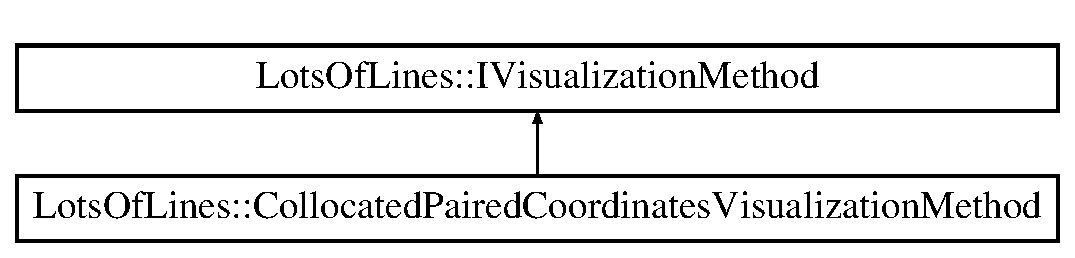
\includegraphics[height=2.000000cm]{class_lots_of_lines_1_1_collocated_paired_coordinates_visualization_method}
\end{center}
\end{figure}
\subsection*{Public Member Functions}
\begin{DoxyCompactItemize}
\item 
void \hyperlink{class_lots_of_lines_1_1_collocated_paired_coordinates_visualization_method_adc262d91a1fb1972a3f7a4dcb6da5ef7}{get\+Navigation\+Options} (\hyperlink{struct_lots_of_lines_1_1_navigation_options}{Navigation\+Options} \&options\+Out)\hypertarget{class_lots_of_lines_1_1_collocated_paired_coordinates_visualization_method_adc262d91a1fb1972a3f7a4dcb6da5ef7}{}\label{class_lots_of_lines_1_1_collocated_paired_coordinates_visualization_method_adc262d91a1fb1972a3f7a4dcb6da5ef7}

\begin{DoxyCompactList}\small\item\em Should return the navigation options for the rendering method (X scroll lock, etc) \end{DoxyCompactList}\item 
bool \hyperlink{class_lots_of_lines_1_1_collocated_paired_coordinates_visualization_method_aa2fc5876109a7fbc2f3e66dde6de8582}{generate\+V\+BO} (const std\+::shared\+\_\+ptr$<$ const \hyperlink{class_lots_of_lines_1_1_data_set}{Data\+Set} $>$ data\+Set, std\+::vector$<$ \hyperlink{struct_lots_of_lines_1_1_vertex}{Vertex} $>$ \&vertices\+Out, std\+::vector$<$ unsigned int $>$ \&indices\+Out, \hyperlink{class_lots_of_lines_1_1_rendering_system}{Rendering\+System} $\ast$driver, const \hyperlink{class_lots_of_lines_1_1_visualization_options}{Visualization\+Options} \&options)\hypertarget{class_lots_of_lines_1_1_collocated_paired_coordinates_visualization_method_aa2fc5876109a7fbc2f3e66dde6de8582}{}\label{class_lots_of_lines_1_1_collocated_paired_coordinates_visualization_method_aa2fc5876109a7fbc2f3e66dde6de8582}

\begin{DoxyCompactList}\small\item\em Generate a vertex buffer for the visualization. \end{DoxyCompactList}\end{DoxyCompactItemize}


The documentation for this class was generated from the following files\+:\begin{DoxyCompactItemize}
\item 
D\+:/\+School/\+C\+W\+U/\+C\+S 481/\+Lots-\/of-\/\+Lines/source/\+Rendering\+System/Collocated\+Paired\+Coordinates\+Visualization\+Method.\+hpp\item 
D\+:/\+School/\+C\+W\+U/\+C\+S 481/\+Lots-\/of-\/\+Lines/source/\+Rendering\+System/Collocated\+Paired\+Coordinates\+Visualization\+Method.\+cpp\end{DoxyCompactItemize}

\hypertarget{class_lots_of_lines_1_1_c_s_v_file_loader}{}\section{Lots\+Of\+Lines\+:\+:C\+S\+V\+File\+Loader Class Reference}
\label{class_lots_of_lines_1_1_c_s_v_file_loader}\index{Lots\+Of\+Lines\+::\+C\+S\+V\+File\+Loader@{Lots\+Of\+Lines\+::\+C\+S\+V\+File\+Loader}}
Inheritance diagram for Lots\+Of\+Lines\+:\+:C\+S\+V\+File\+Loader\+:\begin{figure}[H]
\begin{center}
\leavevmode
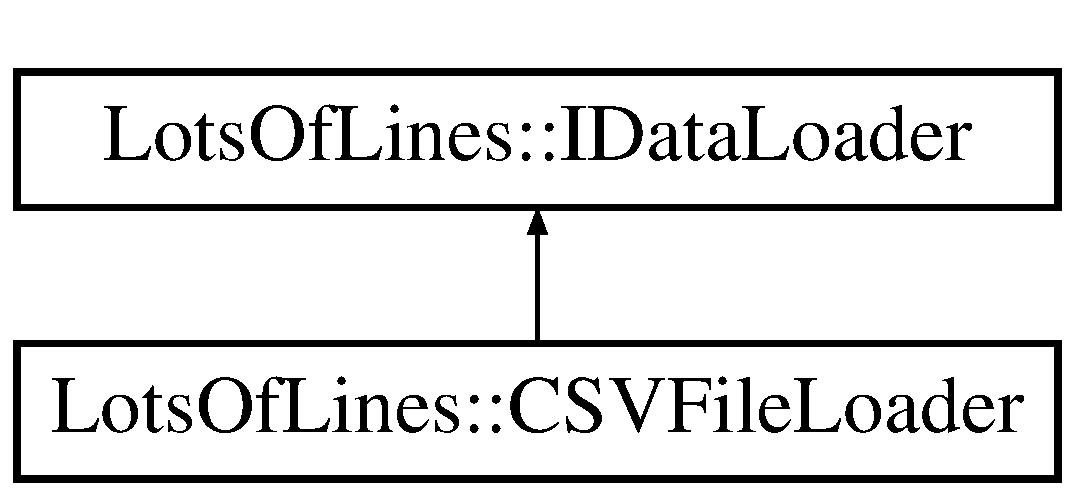
\includegraphics[height=2.000000cm]{class_lots_of_lines_1_1_c_s_v_file_loader}
\end{center}
\end{figure}
\subsection*{Public Member Functions}
\begin{DoxyCompactItemize}
\item 
bool \hyperlink{class_lots_of_lines_1_1_c_s_v_file_loader_a745f53165fdb04a372e2311c8428cc3e}{supports\+Format} (const std\+::string \&path)
\item 
std\+::shared\+\_\+ptr$<$ \hyperlink{class_lots_of_lines_1_1_data_set}{Data\+Set} $>$ \hyperlink{class_lots_of_lines_1_1_c_s_v_file_loader_a7e8c7d04cf7f868ee31fc3b2d79c0a76}{load\+Data} (const std\+::string \&path, const \hyperlink{struct_lots_of_lines_1_1_load_options}{Load\+Options} \&options, \hyperlink{class_lots_of_lines_1_1_progress_message}{Progress\+Message} $\ast$progress) const 
\begin{DoxyCompactList}\small\item\em Load vector data from a source specified by the path and output it as an array of vectors. \end{DoxyCompactList}\end{DoxyCompactItemize}


\subsection{Member Function Documentation}
\index{Lots\+Of\+Lines\+::\+C\+S\+V\+File\+Loader@{Lots\+Of\+Lines\+::\+C\+S\+V\+File\+Loader}!load\+Data@{load\+Data}}
\index{load\+Data@{load\+Data}!Lots\+Of\+Lines\+::\+C\+S\+V\+File\+Loader@{Lots\+Of\+Lines\+::\+C\+S\+V\+File\+Loader}}
\subsubsection[{\texorpdfstring{load\+Data(const std\+::string \&path, const Load\+Options \&options, Progress\+Message $\ast$progress) const }{loadData(const std::string &path, const LoadOptions &options, ProgressMessage *progress) const }}]{\setlength{\rightskip}{0pt plus 5cm}std\+::shared\+\_\+ptr$<$ {\bf Data\+Set} $>$ C\+S\+V\+File\+Loader\+::load\+Data (
\begin{DoxyParamCaption}
\item[{const std\+::string \&}]{path, }
\item[{const {\bf Load\+Options} \&}]{options, }
\item[{{\bf Progress\+Message} $\ast$}]{progress}
\end{DoxyParamCaption}
) const\hspace{0.3cm}{\ttfamily [virtual]}}\hypertarget{class_lots_of_lines_1_1_c_s_v_file_loader_a7e8c7d04cf7f868ee31fc3b2d79c0a76}{}\label{class_lots_of_lines_1_1_c_s_v_file_loader_a7e8c7d04cf7f868ee31fc3b2d79c0a76}


Load vector data from a source specified by the path and output it as an array of vectors. 


\begin{DoxyParams}{Parameters}
{\em path} & The path (file path, U\+RI, etc.) where the data should be loaded from. \\
\hline
\end{DoxyParams}
\begin{DoxyReturn}{Returns}
The \hyperlink{class_lots_of_lines_1_1_data_set}{Data\+Set} or nullptr if an error occurred. 
\end{DoxyReturn}


Implements \hyperlink{class_lots_of_lines_1_1_i_data_loader_ad2e836decbe5d96e0ac2ca43a8177881}{Lots\+Of\+Lines\+::\+I\+Data\+Loader}.

\index{Lots\+Of\+Lines\+::\+C\+S\+V\+File\+Loader@{Lots\+Of\+Lines\+::\+C\+S\+V\+File\+Loader}!supports\+Format@{supports\+Format}}
\index{supports\+Format@{supports\+Format}!Lots\+Of\+Lines\+::\+C\+S\+V\+File\+Loader@{Lots\+Of\+Lines\+::\+C\+S\+V\+File\+Loader}}
\subsubsection[{\texorpdfstring{supports\+Format(const std\+::string \&path)}{supportsFormat(const std::string &path)}}]{\setlength{\rightskip}{0pt plus 5cm}bool C\+S\+V\+File\+Loader\+::supports\+Format (
\begin{DoxyParamCaption}
\item[{const std\+::string \&}]{path}
\end{DoxyParamCaption}
)\hspace{0.3cm}{\ttfamily [virtual]}}\hypertarget{class_lots_of_lines_1_1_c_s_v_file_loader_a745f53165fdb04a372e2311c8428cc3e}{}\label{class_lots_of_lines_1_1_c_s_v_file_loader_a745f53165fdb04a372e2311c8428cc3e}

\begin{DoxyParams}{Parameters}
{\em path} & The path (file path, U\+RI, etc.) where the data will be loaded from. \\
\hline
\end{DoxyParams}
\begin{DoxyReturn}{Returns}
True if this loader supports loading the specified path, false otherwise. 
\end{DoxyReturn}


Implements \hyperlink{class_lots_of_lines_1_1_i_data_loader_a73f9ee96a55bd6d339d5028f951240f9}{Lots\+Of\+Lines\+::\+I\+Data\+Loader}.



The documentation for this class was generated from the following files\+:\begin{DoxyCompactItemize}
\item 
D\+:/\+School/\+C\+W\+U/\+C\+S 481/\+Lots-\/of-\/\+Lines/source/\+Data\+Model/C\+S\+V\+File\+Loader.\+hpp\item 
D\+:/\+School/\+C\+W\+U/\+C\+S 481/\+Lots-\/of-\/\+Lines/source/\+Data\+Model/C\+S\+V\+File\+Loader.\+cpp\end{DoxyCompactItemize}

\hypertarget{class_lots_of_lines_1_1_data_file_loader}{}\section{Lots\+Of\+Lines\+:\+:Data\+File\+Loader Class Reference}
\label{class_lots_of_lines_1_1_data_file_loader}\index{Lots\+Of\+Lines\+::\+Data\+File\+Loader@{Lots\+Of\+Lines\+::\+Data\+File\+Loader}}
Inheritance diagram for Lots\+Of\+Lines\+:\+:Data\+File\+Loader\+:\begin{figure}[H]
\begin{center}
\leavevmode
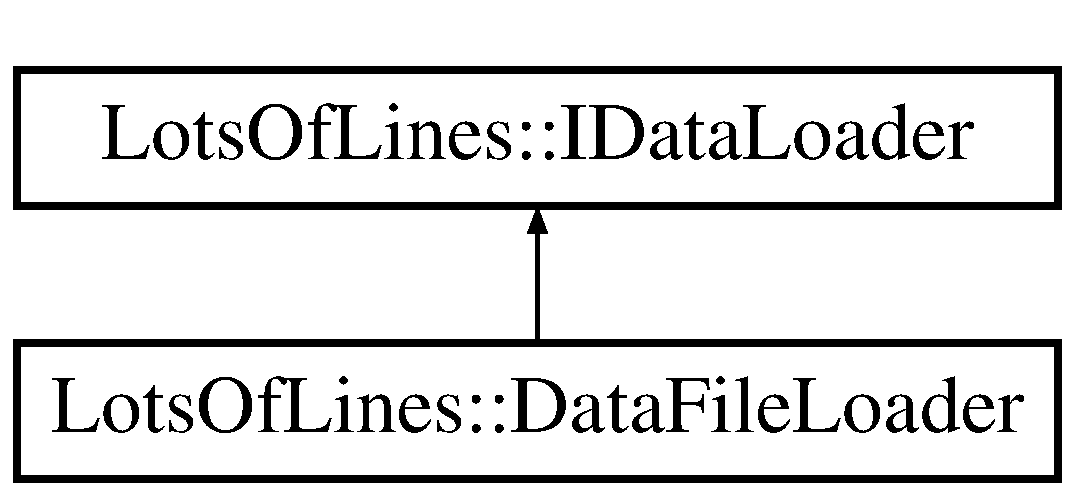
\includegraphics[height=2.000000cm]{class_lots_of_lines_1_1_data_file_loader}
\end{center}
\end{figure}
\subsection*{Public Member Functions}
\begin{DoxyCompactItemize}
\item 
bool \hyperlink{class_lots_of_lines_1_1_data_file_loader_ac515d96c661865355080a999b8de1967}{supports\+Format} (const std\+::string \&path)
\item 
std\+::shared\+\_\+ptr$<$ \hyperlink{class_lots_of_lines_1_1_data_set}{Data\+Set} $>$ \hyperlink{class_lots_of_lines_1_1_data_file_loader_af7f8239a2828d607265cd3c52fcee87b}{load\+Data} (const std\+::string \&path, const \hyperlink{struct_lots_of_lines_1_1_load_options}{Load\+Options} \&options, \hyperlink{class_lots_of_lines_1_1_progress_message}{Progress\+Message} $\ast$progress) const 
\begin{DoxyCompactList}\small\item\em Load vector data from a source specified by the path and output it as an array of vectors. \end{DoxyCompactList}\end{DoxyCompactItemize}


\subsection{Member Function Documentation}
\index{Lots\+Of\+Lines\+::\+Data\+File\+Loader@{Lots\+Of\+Lines\+::\+Data\+File\+Loader}!load\+Data@{load\+Data}}
\index{load\+Data@{load\+Data}!Lots\+Of\+Lines\+::\+Data\+File\+Loader@{Lots\+Of\+Lines\+::\+Data\+File\+Loader}}
\subsubsection[{\texorpdfstring{load\+Data(const std\+::string \&path, const Load\+Options \&options, Progress\+Message $\ast$progress) const }{loadData(const std::string &path, const LoadOptions &options, ProgressMessage *progress) const }}]{\setlength{\rightskip}{0pt plus 5cm}std\+::shared\+\_\+ptr$<$ {\bf Data\+Set} $>$ Data\+File\+Loader\+::load\+Data (
\begin{DoxyParamCaption}
\item[{const std\+::string \&}]{path, }
\item[{const {\bf Load\+Options} \&}]{options, }
\item[{{\bf Progress\+Message} $\ast$}]{progress}
\end{DoxyParamCaption}
) const\hspace{0.3cm}{\ttfamily [virtual]}}\hypertarget{class_lots_of_lines_1_1_data_file_loader_af7f8239a2828d607265cd3c52fcee87b}{}\label{class_lots_of_lines_1_1_data_file_loader_af7f8239a2828d607265cd3c52fcee87b}


Load vector data from a source specified by the path and output it as an array of vectors. 


\begin{DoxyParams}{Parameters}
{\em path} & The path (file path, U\+RI, etc.) where the data should be loaded from. \\
\hline
\end{DoxyParams}
\begin{DoxyReturn}{Returns}
The \hyperlink{class_lots_of_lines_1_1_data_set}{Data\+Set} or nullptr if an error occurred. 
\end{DoxyReturn}


Implements \hyperlink{class_lots_of_lines_1_1_i_data_loader_ad2e836decbe5d96e0ac2ca43a8177881}{Lots\+Of\+Lines\+::\+I\+Data\+Loader}.

\index{Lots\+Of\+Lines\+::\+Data\+File\+Loader@{Lots\+Of\+Lines\+::\+Data\+File\+Loader}!supports\+Format@{supports\+Format}}
\index{supports\+Format@{supports\+Format}!Lots\+Of\+Lines\+::\+Data\+File\+Loader@{Lots\+Of\+Lines\+::\+Data\+File\+Loader}}
\subsubsection[{\texorpdfstring{supports\+Format(const std\+::string \&path)}{supportsFormat(const std::string &path)}}]{\setlength{\rightskip}{0pt plus 5cm}bool Data\+File\+Loader\+::supports\+Format (
\begin{DoxyParamCaption}
\item[{const std\+::string \&}]{path}
\end{DoxyParamCaption}
)\hspace{0.3cm}{\ttfamily [virtual]}}\hypertarget{class_lots_of_lines_1_1_data_file_loader_ac515d96c661865355080a999b8de1967}{}\label{class_lots_of_lines_1_1_data_file_loader_ac515d96c661865355080a999b8de1967}

\begin{DoxyParams}{Parameters}
{\em path} & The path (file path, U\+RI, etc.) where the data will be loaded from. \\
\hline
\end{DoxyParams}
\begin{DoxyReturn}{Returns}
True if this loader supports loading the specified path, false otherwise. 
\end{DoxyReturn}


Implements \hyperlink{class_lots_of_lines_1_1_i_data_loader_a73f9ee96a55bd6d339d5028f951240f9}{Lots\+Of\+Lines\+::\+I\+Data\+Loader}.



The documentation for this class was generated from the following files\+:\begin{DoxyCompactItemize}
\item 
D\+:/\+School/\+C\+W\+U/\+C\+S 481/\+Lots-\/of-\/\+Lines/source/\+Data\+Model/Data\+File\+Loader.\+hpp\item 
D\+:/\+School/\+C\+W\+U/\+C\+S 481/\+Lots-\/of-\/\+Lines/source/\+Data\+Model/Data\+File\+Loader.\+cpp\end{DoxyCompactItemize}

\hypertarget{class_lots_of_lines_1_1_data_model}{}\section{Lots\+Of\+Lines\+:\+:Data\+Model Class Reference}
\label{class_lots_of_lines_1_1_data_model}\index{Lots\+Of\+Lines\+::\+Data\+Model@{Lots\+Of\+Lines\+::\+Data\+Model}}


The \hyperlink{class_lots_of_lines_1_1_data_model}{Data\+Model} class handles loading and processing datasets to convert them to a form usable by the rendering system.  




{\ttfamily \#include $<$Data\+Model.\+hpp$>$}

\subsection*{Public Member Functions}
\begin{DoxyCompactItemize}
\item 
{\bfseries Data\+Model} (const Data\+Loader\+Array \&data\+Loaders)\hypertarget{class_lots_of_lines_1_1_data_model_ad16cc6c51af644c4109ce088d50c6863}{}\label{class_lots_of_lines_1_1_data_model_ad16cc6c51af644c4109ce088d50c6863}

\item 
void \hyperlink{class_lots_of_lines_1_1_data_model_a6a98b1f57a88705c93fd62e439ae0d1b}{register\+Loader} (\hyperlink{class_lots_of_lines_1_1_i_data_loader}{I\+Data\+Loader} $\ast$loader)\hypertarget{class_lots_of_lines_1_1_data_model_a6a98b1f57a88705c93fd62e439ae0d1b}{}\label{class_lots_of_lines_1_1_data_model_a6a98b1f57a88705c93fd62e439ae0d1b}

\begin{DoxyCompactList}\small\item\em Register a data loader with the \hyperlink{class_lots_of_lines_1_1_data_model}{Data\+Model}. Data loaders implement the actual parsing logic. \end{DoxyCompactList}\item 
std\+::shared\+\_\+ptr$<$ \hyperlink{class_lots_of_lines_1_1_data_set}{Data\+Set} $>$ \hyperlink{class_lots_of_lines_1_1_data_model_ab8b8b52feec4ea1331d3efcbe000b148}{load\+Data} (const std\+::string \&path, const \hyperlink{struct_lots_of_lines_1_1_load_options}{Load\+Options} \&options=Load\+Options\+::default, \hyperlink{class_lots_of_lines_1_1_progress_message}{Progress\+Message} $\ast$progress=nullptr) const 
\begin{DoxyCompactList}\small\item\em Loads data from the specified source. \end{DoxyCompactList}\end{DoxyCompactItemize}


\subsection{Detailed Description}
The \hyperlink{class_lots_of_lines_1_1_data_model}{Data\+Model} class handles loading and processing datasets to convert them to a form usable by the rendering system. 

\subsection{Member Function Documentation}
\index{Lots\+Of\+Lines\+::\+Data\+Model@{Lots\+Of\+Lines\+::\+Data\+Model}!load\+Data@{load\+Data}}
\index{load\+Data@{load\+Data}!Lots\+Of\+Lines\+::\+Data\+Model@{Lots\+Of\+Lines\+::\+Data\+Model}}
\subsubsection[{\texorpdfstring{load\+Data(const std\+::string \&path, const Load\+Options \&options=\+Load\+Options\+::default, Progress\+Message $\ast$progress=nullptr) const }{loadData(const std::string &path, const LoadOptions &options=LoadOptions::default, ProgressMessage *progress=nullptr) const }}]{\setlength{\rightskip}{0pt plus 5cm}std\+::shared\+\_\+ptr$<$ {\bf Data\+Set} $>$ Data\+Model\+::load\+Data (
\begin{DoxyParamCaption}
\item[{const std\+::string \&}]{path, }
\item[{const {\bf Load\+Options} \&}]{options = {\ttfamily LoadOptions\+:\+:default}, }
\item[{{\bf Progress\+Message} $\ast$}]{progress = {\ttfamily nullptr}}
\end{DoxyParamCaption}
) const}\hypertarget{class_lots_of_lines_1_1_data_model_ab8b8b52feec4ea1331d3efcbe000b148}{}\label{class_lots_of_lines_1_1_data_model_ab8b8b52feec4ea1331d3efcbe000b148}


Loads data from the specified source. 


\begin{DoxyParams}{Parameters}
{\em path} & The path to load data from. The format of this parameter is to be interpreted by the loader implementation and could be a file path, a U\+RL, or something else. \\
\hline
\end{DoxyParams}
\begin{DoxyReturn}{Returns}
A shared\+\_\+ptr to the \hyperlink{class_lots_of_lines_1_1_data_set}{Data\+Set} loaded from the path, or nullptr if an error occurred. 
\end{DoxyReturn}


The documentation for this class was generated from the following files\+:\begin{DoxyCompactItemize}
\item 
D\+:/\+School/\+C\+W\+U/\+C\+S 481/\+Lots-\/of-\/\+Lines/source/\+Data\+Model/Data\+Model.\+hpp\item 
D\+:/\+School/\+C\+W\+U/\+C\+S 481/\+Lots-\/of-\/\+Lines/source/\+Data\+Model/Data\+Model.\+cpp\end{DoxyCompactItemize}

\hypertarget{class_lots_of_lines_1_1_data_set}{}\section{Lots\+Of\+Lines\+:\+:Data\+Set Class Reference}
\label{class_lots_of_lines_1_1_data_set}\index{Lots\+Of\+Lines\+::\+Data\+Set@{Lots\+Of\+Lines\+::\+Data\+Set}}


\hyperlink{class_lots_of_lines_1_1_data_set}{Data\+Set} holds the data for multiple classes of vector data.  




{\ttfamily \#include $<$Data\+Set.\+hpp$>$}

\subsection*{Classes}
\begin{DoxyCompactItemize}
\item 
class \hyperlink{class_lots_of_lines_1_1_data_set_1_1_iterator}{Iterator}
\begin{DoxyCompactList}\small\item\em \hyperlink{class_lots_of_lines_1_1_data_set_1_1_iterator}{Iterator} class for traversing the dataset easier. \end{DoxyCompactList}\end{DoxyCompactItemize}
\subsection*{Public Member Functions}
\begin{DoxyCompactItemize}
\item 
\hyperlink{class_lots_of_lines_1_1_data_set_1_1_iterator}{Iterator} \hyperlink{class_lots_of_lines_1_1_data_set_a10b7e2e1319d223c6365c5acec9a3f3a}{iterator} () const 
\item 
unsigned int \hyperlink{class_lots_of_lines_1_1_data_set_a014a459b9e76b953e541f4d528fc7cdb}{vector\+Count} () const 
\item 
Vector \& \hyperlink{class_lots_of_lines_1_1_data_set_a65f1a6baa7516118f6fb21f0329ab053}{get\+Vector} (unsigned int idx)
\item 
const Vector \& \hyperlink{class_lots_of_lines_1_1_data_set_a2f748da99b96d226d5d4e8903da5db10}{get\+Vector} (unsigned int idx) const 
\item 
Vector \& \hyperlink{class_lots_of_lines_1_1_data_set_ad15f040e5048686fb2e28c3e2a38775c}{operator\mbox{[}$\,$\mbox{]}} (unsigned int idx)\hypertarget{class_lots_of_lines_1_1_data_set_ad15f040e5048686fb2e28c3e2a38775c}{}\label{class_lots_of_lines_1_1_data_set_ad15f040e5048686fb2e28c3e2a38775c}

\begin{DoxyCompactList}\small\item\em subscript operator for accessing vectors at the specified index. \end{DoxyCompactList}\item 
const Vector \& \hyperlink{class_lots_of_lines_1_1_data_set_aec5ed23bf96864526ff4a62f94767ce5}{operator\mbox{[}$\,$\mbox{]}} (unsigned int idx) const \hypertarget{class_lots_of_lines_1_1_data_set_aec5ed23bf96864526ff4a62f94767ce5}{}\label{class_lots_of_lines_1_1_data_set_aec5ed23bf96864526ff4a62f94767ce5}

\begin{DoxyCompactList}\small\item\em subscript operator for accessing vectors at the specified index. \end{DoxyCompactList}\item 
\hyperlink{class_lots_of_lines_1_1_data_set_ac9b99505bafd5b1cccf8a361c3ac84a7}{Data\+Set} ()\hypertarget{class_lots_of_lines_1_1_data_set_ac9b99505bafd5b1cccf8a361c3ac84a7}{}\label{class_lots_of_lines_1_1_data_set_ac9b99505bafd5b1cccf8a361c3ac84a7}

\begin{DoxyCompactList}\small\item\em Default constructor to make. \end{DoxyCompactList}\item 
unsigned int \hyperlink{class_lots_of_lines_1_1_data_set_aff429ddd61367950bd1289fbcd095de2}{add\+Vector\+Class} (const std\+::string \&name)
\begin{DoxyCompactList}\small\item\em Add a vector class to the dataset. \end{DoxyCompactList}\item 
unsigned int \hyperlink{class_lots_of_lines_1_1_data_set_a574346ae47374acdf9a177dca226365b}{get\+Class\+Index} (const std\+::string \&name)\hypertarget{class_lots_of_lines_1_1_data_set_a574346ae47374acdf9a177dca226365b}{}\label{class_lots_of_lines_1_1_data_set_a574346ae47374acdf9a177dca226365b}

\begin{DoxyCompactList}\small\item\em Get class index from the class name. \end{DoxyCompactList}\item 
void \hyperlink{class_lots_of_lines_1_1_data_set_a4f12b125c969da469677f8a5ec6be10d}{add\+Vector} (const Vector \&vec, const std\+::string \&vector\+Class=\char`\"{}default\char`\"{})
\begin{DoxyCompactList}\small\item\em Add a vector to the specified class. \end{DoxyCompactList}\item 
const Vector \& {\bfseries get\+Max\+Values} () const \hypertarget{class_lots_of_lines_1_1_data_set_a7c495cd8a0d584ffc352b4fbd84c6e4f}{}\label{class_lots_of_lines_1_1_data_set_a7c495cd8a0d584ffc352b4fbd84c6e4f}

\item 
const Vector \& {\bfseries get\+Min\+Values} () const \hypertarget{class_lots_of_lines_1_1_data_set_afa668a139d080386883302ee8ef03f5a}{}\label{class_lots_of_lines_1_1_data_set_afa668a139d080386883302ee8ef03f5a}

\item 
void \hyperlink{class_lots_of_lines_1_1_data_set_a4a6256527dafe3081619a48902c299bb}{normalize\+Data} (E\+\_\+\+D\+A\+T\+A\+\_\+\+N\+O\+R\+M\+A\+L\+I\+Z\+A\+T\+I\+O\+N\+\_\+\+M\+O\+DE mode)\hypertarget{class_lots_of_lines_1_1_data_set_a4a6256527dafe3081619a48902c299bb}{}\label{class_lots_of_lines_1_1_data_set_a4a6256527dafe3081619a48902c299bb}

\begin{DoxyCompactList}\small\item\em Normalize the vector data to the -\/1.\+0 to 1.\+0 range. This should only be called once all vectors have been loaded to the dataset. \end{DoxyCompactList}\end{DoxyCompactItemize}


\subsection{Detailed Description}
\hyperlink{class_lots_of_lines_1_1_data_set}{Data\+Set} holds the data for multiple classes of vector data. 

\subsection{Member Function Documentation}
\index{Lots\+Of\+Lines\+::\+Data\+Set@{Lots\+Of\+Lines\+::\+Data\+Set}!add\+Vector@{add\+Vector}}
\index{add\+Vector@{add\+Vector}!Lots\+Of\+Lines\+::\+Data\+Set@{Lots\+Of\+Lines\+::\+Data\+Set}}
\subsubsection[{\texorpdfstring{add\+Vector(const Vector \&vec, const std\+::string \&vector\+Class=""default"")}{addVector(const Vector &vec, const std::string &vectorClass="default")}}]{\setlength{\rightskip}{0pt plus 5cm}void Data\+Set\+::add\+Vector (
\begin{DoxyParamCaption}
\item[{const Vector \&}]{vec, }
\item[{const std\+::string \&}]{vector\+Class = {\ttfamily \char`\"{}default\char`\"{}}}
\end{DoxyParamCaption}
)}\hypertarget{class_lots_of_lines_1_1_data_set_a4f12b125c969da469677f8a5ec6be10d}{}\label{class_lots_of_lines_1_1_data_set_a4f12b125c969da469677f8a5ec6be10d}


Add a vector to the specified class. 


\begin{DoxyParams}{Parameters}
{\em vector\+Class} & Data class name. \\
\hline
{\em vec} & The vector data to add. \\
\hline
\end{DoxyParams}
\index{Lots\+Of\+Lines\+::\+Data\+Set@{Lots\+Of\+Lines\+::\+Data\+Set}!add\+Vector\+Class@{add\+Vector\+Class}}
\index{add\+Vector\+Class@{add\+Vector\+Class}!Lots\+Of\+Lines\+::\+Data\+Set@{Lots\+Of\+Lines\+::\+Data\+Set}}
\subsubsection[{\texorpdfstring{add\+Vector\+Class(const std\+::string \&name)}{addVectorClass(const std::string &name)}}]{\setlength{\rightskip}{0pt plus 5cm}unsigned int Data\+Set\+::add\+Vector\+Class (
\begin{DoxyParamCaption}
\item[{const std\+::string \&}]{name}
\end{DoxyParamCaption}
)}\hypertarget{class_lots_of_lines_1_1_data_set_aff429ddd61367950bd1289fbcd095de2}{}\label{class_lots_of_lines_1_1_data_set_aff429ddd61367950bd1289fbcd095de2}


Add a vector class to the dataset. 

\begin{DoxyReturn}{Returns}
The index of the vector class that was added. 
\end{DoxyReturn}
\index{Lots\+Of\+Lines\+::\+Data\+Set@{Lots\+Of\+Lines\+::\+Data\+Set}!get\+Vector@{get\+Vector}}
\index{get\+Vector@{get\+Vector}!Lots\+Of\+Lines\+::\+Data\+Set@{Lots\+Of\+Lines\+::\+Data\+Set}}
\subsubsection[{\texorpdfstring{get\+Vector(unsigned int idx)}{getVector(unsigned int idx)}}]{\setlength{\rightskip}{0pt plus 5cm}Vector \& Data\+Set\+::get\+Vector (
\begin{DoxyParamCaption}
\item[{unsigned int}]{idx}
\end{DoxyParamCaption}
)}\hypertarget{class_lots_of_lines_1_1_data_set_a65f1a6baa7516118f6fb21f0329ab053}{}\label{class_lots_of_lines_1_1_data_set_a65f1a6baa7516118f6fb21f0329ab053}
\begin{DoxyReturn}{Returns}
The vector at the specified index. 
\end{DoxyReturn}
\index{Lots\+Of\+Lines\+::\+Data\+Set@{Lots\+Of\+Lines\+::\+Data\+Set}!get\+Vector@{get\+Vector}}
\index{get\+Vector@{get\+Vector}!Lots\+Of\+Lines\+::\+Data\+Set@{Lots\+Of\+Lines\+::\+Data\+Set}}
\subsubsection[{\texorpdfstring{get\+Vector(unsigned int idx) const }{getVector(unsigned int idx) const }}]{\setlength{\rightskip}{0pt plus 5cm}const Vector \& Data\+Set\+::get\+Vector (
\begin{DoxyParamCaption}
\item[{unsigned int}]{idx}
\end{DoxyParamCaption}
) const}\hypertarget{class_lots_of_lines_1_1_data_set_a2f748da99b96d226d5d4e8903da5db10}{}\label{class_lots_of_lines_1_1_data_set_a2f748da99b96d226d5d4e8903da5db10}
\begin{DoxyReturn}{Returns}
The vector at the specified index. 
\end{DoxyReturn}
\index{Lots\+Of\+Lines\+::\+Data\+Set@{Lots\+Of\+Lines\+::\+Data\+Set}!iterator@{iterator}}
\index{iterator@{iterator}!Lots\+Of\+Lines\+::\+Data\+Set@{Lots\+Of\+Lines\+::\+Data\+Set}}
\subsubsection[{\texorpdfstring{iterator() const }{iterator() const }}]{\setlength{\rightskip}{0pt plus 5cm}{\bf Data\+Set\+::\+Iterator} Data\+Set\+::iterator (
\begin{DoxyParamCaption}
{}
\end{DoxyParamCaption}
) const}\hypertarget{class_lots_of_lines_1_1_data_set_a10b7e2e1319d223c6365c5acec9a3f3a}{}\label{class_lots_of_lines_1_1_data_set_a10b7e2e1319d223c6365c5acec9a3f3a}
\begin{DoxyReturn}{Returns}
An iterator that can be used to traverse this dataset. 
\end{DoxyReturn}
\index{Lots\+Of\+Lines\+::\+Data\+Set@{Lots\+Of\+Lines\+::\+Data\+Set}!vector\+Count@{vector\+Count}}
\index{vector\+Count@{vector\+Count}!Lots\+Of\+Lines\+::\+Data\+Set@{Lots\+Of\+Lines\+::\+Data\+Set}}
\subsubsection[{\texorpdfstring{vector\+Count() const }{vectorCount() const }}]{\setlength{\rightskip}{0pt plus 5cm}unsigned int Data\+Set\+::vector\+Count (
\begin{DoxyParamCaption}
{}
\end{DoxyParamCaption}
) const}\hypertarget{class_lots_of_lines_1_1_data_set_a014a459b9e76b953e541f4d528fc7cdb}{}\label{class_lots_of_lines_1_1_data_set_a014a459b9e76b953e541f4d528fc7cdb}
\begin{DoxyReturn}{Returns}
The number of vectors in the dataset 
\end{DoxyReturn}


The documentation for this class was generated from the following files\+:\begin{DoxyCompactItemize}
\item 
D\+:/\+School/\+C\+W\+U/\+C\+S 481/\+Lots-\/of-\/\+Lines/source/\+Data\+Model/Data\+Set.\+hpp\item 
D\+:/\+School/\+C\+W\+U/\+C\+S 481/\+Lots-\/of-\/\+Lines/source/\+Data\+Model/Data\+Set.\+cpp\end{DoxyCompactItemize}

\hypertarget{class_data_table_model}{}\section{Data\+Table\+Model Class Reference}
\label{class_data_table_model}\index{Data\+Table\+Model@{Data\+Table\+Model}}


Qt table model for showing one vector class of a Data\+Set.  




{\ttfamily \#include $<$Data\+Table\+Model.\+h$>$}

Inheritance diagram for Data\+Table\+Model\+:\begin{figure}[H]
\begin{center}
\leavevmode
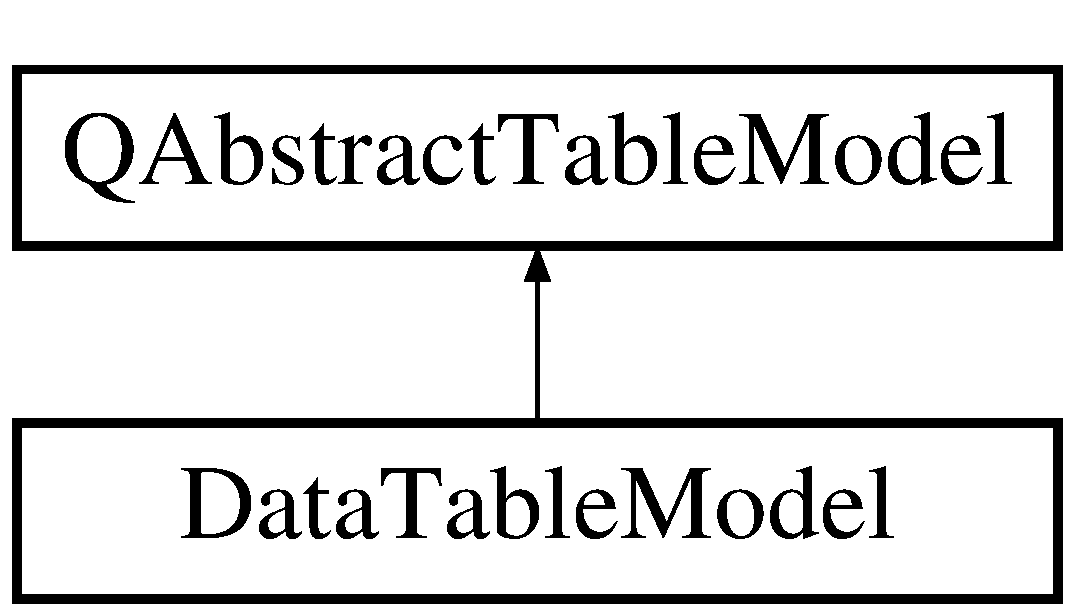
\includegraphics[height=2.000000cm]{class_data_table_model}
\end{center}
\end{figure}
\subsection*{Public Member Functions}
\begin{DoxyCompactItemize}
\item 
{\bfseries Data\+Table\+Model} (std\+::shared\+\_\+ptr$<$ \hyperlink{class_lots_of_lines_1_1_data_set}{Lots\+Of\+Lines\+::\+Data\+Set} $>$ data\+Set)\hypertarget{class_data_table_model_a9887aeddc9dccb859088f489d7256382}{}\label{class_data_table_model_a9887aeddc9dccb859088f489d7256382}

\item 
int {\bfseries row\+Count} (const Q\+Model\+Index \&) const \hypertarget{class_data_table_model_a6d4d1992ec2a0e0a7383c24a303441d9}{}\label{class_data_table_model_a6d4d1992ec2a0e0a7383c24a303441d9}

\item 
int {\bfseries column\+Count} (const Q\+Model\+Index \&) const \hypertarget{class_data_table_model_a1fcc264e8a9f32ed21514f0bfe048ef4}{}\label{class_data_table_model_a1fcc264e8a9f32ed21514f0bfe048ef4}

\item 
Q\+Variant {\bfseries data} (const Q\+Model\+Index \&index, int role=Qt\+::\+Display\+Role) const \hypertarget{class_data_table_model_afb7afd448abaca507716b9042f97709a}{}\label{class_data_table_model_afb7afd448abaca507716b9042f97709a}

\end{DoxyCompactItemize}


\subsection{Detailed Description}
Qt table model for showing one vector class of a Data\+Set. 

The documentation for this class was generated from the following files\+:\begin{DoxyCompactItemize}
\item 
D\+:/\+School/\+C\+W\+U/\+C\+S 481/\+Lots-\/of-\/\+Lines/source/Data\+Table\+Model.\+h\item 
D\+:/\+School/\+C\+W\+U/\+C\+S 481/\+Lots-\/of-\/\+Lines/source/Data\+Table\+Model.\+cpp\end{DoxyCompactItemize}

\hypertarget{class_lots_of_lines_1_1_i_data_loader}{}\section{Lots\+Of\+Lines\+:\+:I\+Data\+Loader Class Reference}
\label{class_lots_of_lines_1_1_i_data_loader}\index{Lots\+Of\+Lines\+::\+I\+Data\+Loader@{Lots\+Of\+Lines\+::\+I\+Data\+Loader}}
Inheritance diagram for Lots\+Of\+Lines\+:\+:I\+Data\+Loader\+:\begin{figure}[H]
\begin{center}
\leavevmode
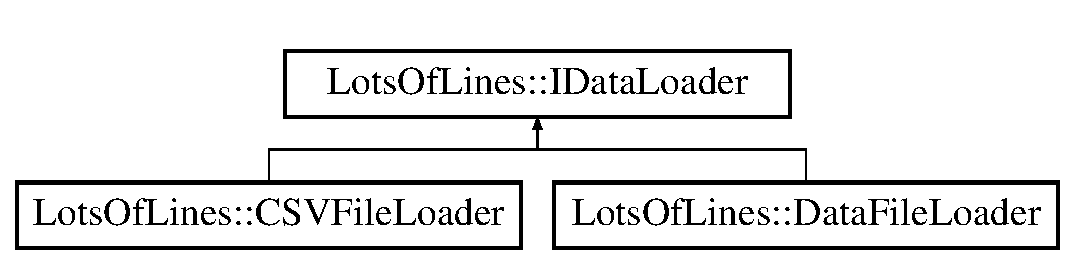
\includegraphics[height=2.000000cm]{class_lots_of_lines_1_1_i_data_loader}
\end{center}
\end{figure}
\subsection*{Public Member Functions}
\begin{DoxyCompactItemize}
\item 
virtual bool \hyperlink{class_lots_of_lines_1_1_i_data_loader_a73f9ee96a55bd6d339d5028f951240f9}{supports\+Format} (const std\+::string \&path)=0
\item 
virtual std\+::shared\+\_\+ptr$<$ \hyperlink{class_lots_of_lines_1_1_data_set}{Data\+Set} $>$ \hyperlink{class_lots_of_lines_1_1_i_data_loader_ad2e836decbe5d96e0ac2ca43a8177881}{load\+Data} (const std\+::string \&path, const \hyperlink{struct_lots_of_lines_1_1_load_options}{Load\+Options} \&options, \hyperlink{class_lots_of_lines_1_1_progress_message}{Progress\+Message} $\ast$progress) const  =0
\begin{DoxyCompactList}\small\item\em Load vector data from a source specified by the path and output it as an array of vectors. \end{DoxyCompactList}\end{DoxyCompactItemize}


\subsection{Member Function Documentation}
\index{Lots\+Of\+Lines\+::\+I\+Data\+Loader@{Lots\+Of\+Lines\+::\+I\+Data\+Loader}!load\+Data@{load\+Data}}
\index{load\+Data@{load\+Data}!Lots\+Of\+Lines\+::\+I\+Data\+Loader@{Lots\+Of\+Lines\+::\+I\+Data\+Loader}}
\subsubsection[{\texorpdfstring{load\+Data(const std\+::string \&path, const Load\+Options \&options, Progress\+Message $\ast$progress) const  =0}{loadData(const std::string &path, const LoadOptions &options, ProgressMessage *progress) const  =0}}]{\setlength{\rightskip}{0pt plus 5cm}virtual std\+::shared\+\_\+ptr$<${\bf Data\+Set}$>$ Lots\+Of\+Lines\+::\+I\+Data\+Loader\+::load\+Data (
\begin{DoxyParamCaption}
\item[{const std\+::string \&}]{path, }
\item[{const {\bf Load\+Options} \&}]{options, }
\item[{{\bf Progress\+Message} $\ast$}]{progress}
\end{DoxyParamCaption}
) const\hspace{0.3cm}{\ttfamily [pure virtual]}}\hypertarget{class_lots_of_lines_1_1_i_data_loader_ad2e836decbe5d96e0ac2ca43a8177881}{}\label{class_lots_of_lines_1_1_i_data_loader_ad2e836decbe5d96e0ac2ca43a8177881}


Load vector data from a source specified by the path and output it as an array of vectors. 


\begin{DoxyParams}{Parameters}
{\em path} & The path (file path, U\+RI, etc.) where the data should be loaded from. \\
\hline
\end{DoxyParams}
\begin{DoxyReturn}{Returns}
The \hyperlink{class_lots_of_lines_1_1_data_set}{Data\+Set} or nullptr if an error occurred. 
\end{DoxyReturn}


Implemented in \hyperlink{class_lots_of_lines_1_1_c_s_v_file_loader_a7e8c7d04cf7f868ee31fc3b2d79c0a76}{Lots\+Of\+Lines\+::\+C\+S\+V\+File\+Loader}, and \hyperlink{class_lots_of_lines_1_1_data_file_loader_af7f8239a2828d607265cd3c52fcee87b}{Lots\+Of\+Lines\+::\+Data\+File\+Loader}.

\index{Lots\+Of\+Lines\+::\+I\+Data\+Loader@{Lots\+Of\+Lines\+::\+I\+Data\+Loader}!supports\+Format@{supports\+Format}}
\index{supports\+Format@{supports\+Format}!Lots\+Of\+Lines\+::\+I\+Data\+Loader@{Lots\+Of\+Lines\+::\+I\+Data\+Loader}}
\subsubsection[{\texorpdfstring{supports\+Format(const std\+::string \&path)=0}{supportsFormat(const std::string &path)=0}}]{\setlength{\rightskip}{0pt plus 5cm}virtual bool Lots\+Of\+Lines\+::\+I\+Data\+Loader\+::supports\+Format (
\begin{DoxyParamCaption}
\item[{const std\+::string \&}]{path}
\end{DoxyParamCaption}
)\hspace{0.3cm}{\ttfamily [pure virtual]}}\hypertarget{class_lots_of_lines_1_1_i_data_loader_a73f9ee96a55bd6d339d5028f951240f9}{}\label{class_lots_of_lines_1_1_i_data_loader_a73f9ee96a55bd6d339d5028f951240f9}

\begin{DoxyParams}{Parameters}
{\em path} & The path (file path, U\+RI, etc.) where the data will be loaded from. \\
\hline
\end{DoxyParams}
\begin{DoxyReturn}{Returns}
True if this loader supports loading the specified path, false otherwise. 
\end{DoxyReturn}


Implemented in \hyperlink{class_lots_of_lines_1_1_c_s_v_file_loader_a745f53165fdb04a372e2311c8428cc3e}{Lots\+Of\+Lines\+::\+C\+S\+V\+File\+Loader}, and \hyperlink{class_lots_of_lines_1_1_data_file_loader_ac515d96c661865355080a999b8de1967}{Lots\+Of\+Lines\+::\+Data\+File\+Loader}.



The documentation for this class was generated from the following file\+:\begin{DoxyCompactItemize}
\item 
D\+:/\+School/\+C\+W\+U/\+C\+S 481/\+Lots-\/of-\/\+Lines/source/\+Data\+Model/I\+Data\+Loader.\+hpp\end{DoxyCompactItemize}

\hypertarget{class_lots_of_lines_1_1_i_renderer}{}\section{Lots\+Of\+Lines\+:\+:I\+Renderer Class Reference}
\label{class_lots_of_lines_1_1_i_renderer}\index{Lots\+Of\+Lines\+::\+I\+Renderer@{Lots\+Of\+Lines\+::\+I\+Renderer}}
Inheritance diagram for Lots\+Of\+Lines\+:\+:I\+Renderer\+:\begin{figure}[H]
\begin{center}
\leavevmode
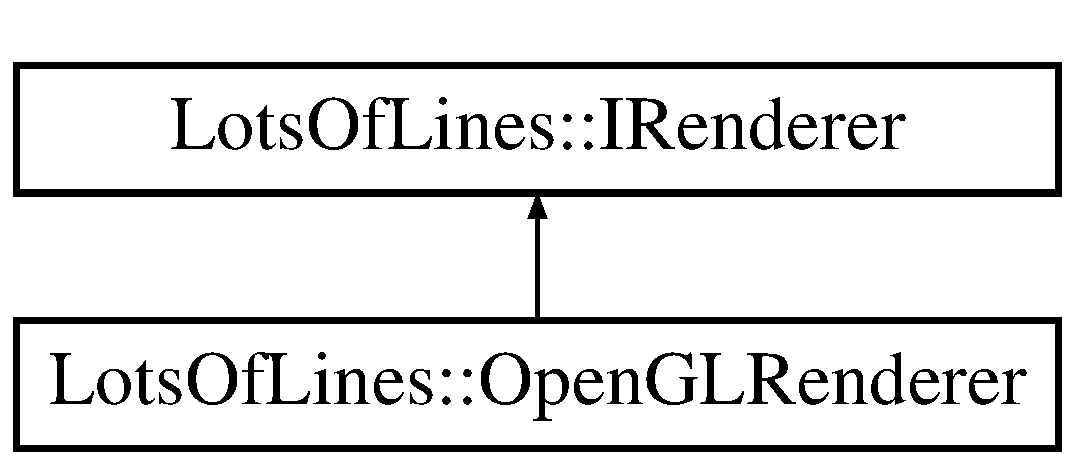
\includegraphics[height=2.000000cm]{class_lots_of_lines_1_1_i_renderer}
\end{center}
\end{figure}
\subsection*{Public Member Functions}
\begin{DoxyCompactItemize}
\item 
virtual bool \hyperlink{class_lots_of_lines_1_1_i_renderer_adc6015bfdf756f4adc59805482b71715}{init} ()=0\hypertarget{class_lots_of_lines_1_1_i_renderer_adc6015bfdf756f4adc59805482b71715}{}\label{class_lots_of_lines_1_1_i_renderer_adc6015bfdf756f4adc59805482b71715}

\begin{DoxyCompactList}\small\item\em Initialize the rendering driver by setting up default shaders and rendering states. \end{DoxyCompactList}\item 
virtual void \hyperlink{class_lots_of_lines_1_1_i_renderer_a076759fc7971de5b7deed588f1d104be}{clear\+Screen} (float r, float g, float b)=0\hypertarget{class_lots_of_lines_1_1_i_renderer_a076759fc7971de5b7deed588f1d104be}{}\label{class_lots_of_lines_1_1_i_renderer_a076759fc7971de5b7deed588f1d104be}

\begin{DoxyCompactList}\small\item\em Clears the screen before re-\/rendering. \end{DoxyCompactList}\item 
virtual void \hyperlink{class_lots_of_lines_1_1_i_renderer_a87dd1fd9695ec5722e4201527075aa51}{begin\+Draw} ()=0\hypertarget{class_lots_of_lines_1_1_i_renderer_a87dd1fd9695ec5722e4201527075aa51}{}\label{class_lots_of_lines_1_1_i_renderer_a87dd1fd9695ec5722e4201527075aa51}

\begin{DoxyCompactList}\small\item\em Sets up rendering states to begin a frame. \end{DoxyCompactList}\item 
virtual void \hyperlink{class_lots_of_lines_1_1_i_renderer_a3f06c10327391ac4f8ad9931409cdda8}{end\+Draw} ()=0\hypertarget{class_lots_of_lines_1_1_i_renderer_a3f06c10327391ac4f8ad9931409cdda8}{}\label{class_lots_of_lines_1_1_i_renderer_a3f06c10327391ac4f8ad9931409cdda8}

\begin{DoxyCompactList}\small\item\em Flips buffers to screen. \end{DoxyCompactList}\item 
virtual void \hyperlink{class_lots_of_lines_1_1_i_renderer_aabdce3cb566a653d8b47a9c6ba13a8f0}{set\+Class\+Colors} (float $\ast$colors)=0\hypertarget{class_lots_of_lines_1_1_i_renderer_aabdce3cb566a653d8b47a9c6ba13a8f0}{}\label{class_lots_of_lines_1_1_i_renderer_aabdce3cb566a653d8b47a9c6ba13a8f0}

\begin{DoxyCompactList}\small\item\em Set the 10x3 array of floats for colors to use when rendering the data class. \end{DoxyCompactList}\item 
virtual void \hyperlink{class_lots_of_lines_1_1_i_renderer_a4aa103c72ba9761bd035401bd744964f}{set\+Viewport} (unsigned int x, unsigned int y, unsigned int width, unsigned int height)=0\hypertarget{class_lots_of_lines_1_1_i_renderer_a4aa103c72ba9761bd035401bd744964f}{}\label{class_lots_of_lines_1_1_i_renderer_a4aa103c72ba9761bd035401bd744964f}

\begin{DoxyCompactList}\small\item\em Set the viewport. \end{DoxyCompactList}\item 
virtual void \hyperlink{class_lots_of_lines_1_1_i_renderer_ada3a02fd728d85fd3e16485dd0b10cf5}{set\+Model\+View\+Projection} (const glm\+::mat4x4 \&mvp)=0\hypertarget{class_lots_of_lines_1_1_i_renderer_ada3a02fd728d85fd3e16485dd0b10cf5}{}\label{class_lots_of_lines_1_1_i_renderer_ada3a02fd728d85fd3e16485dd0b10cf5}

\begin{DoxyCompactList}\small\item\em Set model$\ast$view$\ast$projection matrix. \end{DoxyCompactList}\item 
virtual const glm\+::mat4x4 \& \hyperlink{class_lots_of_lines_1_1_i_renderer_ac2c690247d805c68839ec7a831133665}{get\+Model\+View\+Projection} () const  =0
\item 
virtual \hyperlink{class_lots_of_lines_1_1_i_shader}{I\+Shader} $\ast$ \hyperlink{class_lots_of_lines_1_1_i_renderer_aa3d81559cc4d78fbf1dfdd85a7f34580}{create\+Shader} ()=0\hypertarget{class_lots_of_lines_1_1_i_renderer_aa3d81559cc4d78fbf1dfdd85a7f34580}{}\label{class_lots_of_lines_1_1_i_renderer_aa3d81559cc4d78fbf1dfdd85a7f34580}

\begin{DoxyCompactList}\small\item\em Create a new shader object. \end{DoxyCompactList}\item 
virtual void \hyperlink{class_lots_of_lines_1_1_i_renderer_a5ba7bf13e1fcdbfc7a8a0696a16b1a45}{set\+Shader} (\hyperlink{class_lots_of_lines_1_1_i_shader}{I\+Shader} $\ast$shader)=0\hypertarget{class_lots_of_lines_1_1_i_renderer_a5ba7bf13e1fcdbfc7a8a0696a16b1a45}{}\label{class_lots_of_lines_1_1_i_renderer_a5ba7bf13e1fcdbfc7a8a0696a16b1a45}

\begin{DoxyCompactList}\small\item\em Set the shader program to draw with. \end{DoxyCompactList}\item 
virtual void \hyperlink{class_lots_of_lines_1_1_i_renderer_a9d24612fea435f65dcf7d013e6693b2a}{draw\+V\+BO} (std\+::shared\+\_\+ptr$<$ \hyperlink{class_lots_of_lines_1_1_i_vertex_buffer_object}{I\+Vertex\+Buffer\+Object} $>$ vbo, bool lines=true)=0
\begin{DoxyCompactList}\small\item\em Draw a V\+BO to the screen. \end{DoxyCompactList}\item 
virtual std\+::shared\+\_\+ptr$<$ \hyperlink{class_lots_of_lines_1_1_i_vertex_buffer_object}{I\+Vertex\+Buffer\+Object} $>$ \hyperlink{class_lots_of_lines_1_1_i_renderer_a0e9e0b2bc328bd13f88fea74da6e8abc}{create\+V\+BO} (const std\+::vector$<$ \hyperlink{struct_lots_of_lines_1_1_vertex}{Vertex} $>$ \&vertices, const std\+::vector$<$ unsigned int $>$ \&indices)=0\hypertarget{class_lots_of_lines_1_1_i_renderer_a0e9e0b2bc328bd13f88fea74da6e8abc}{}\label{class_lots_of_lines_1_1_i_renderer_a0e9e0b2bc328bd13f88fea74da6e8abc}

\begin{DoxyCompactList}\small\item\em Construct a V\+BO from a list of vertices and indices. \end{DoxyCompactList}\end{DoxyCompactItemize}
\subsection*{Protected Attributes}
\begin{DoxyCompactItemize}
\item 
\hyperlink{class_lots_of_lines_1_1_rendering_system}{Rendering\+System} $\ast$ {\bfseries m\+\_\+rendering\+System}\hypertarget{class_lots_of_lines_1_1_i_renderer_a0bb52a5e85e8f701b5b846d9286c08f5}{}\label{class_lots_of_lines_1_1_i_renderer_a0bb52a5e85e8f701b5b846d9286c08f5}

\end{DoxyCompactItemize}
\subsection*{Friends}
\begin{DoxyCompactItemize}
\item 
class {\bfseries Rendering\+System}\hypertarget{class_lots_of_lines_1_1_i_renderer_a8973bdd326799bb9e3e2d3bf6c98778d}{}\label{class_lots_of_lines_1_1_i_renderer_a8973bdd326799bb9e3e2d3bf6c98778d}

\end{DoxyCompactItemize}


\subsection{Member Function Documentation}
\index{Lots\+Of\+Lines\+::\+I\+Renderer@{Lots\+Of\+Lines\+::\+I\+Renderer}!draw\+V\+BO@{draw\+V\+BO}}
\index{draw\+V\+BO@{draw\+V\+BO}!Lots\+Of\+Lines\+::\+I\+Renderer@{Lots\+Of\+Lines\+::\+I\+Renderer}}
\subsubsection[{\texorpdfstring{draw\+V\+B\+O(std\+::shared\+\_\+ptr$<$ I\+Vertex\+Buffer\+Object $>$ vbo, bool lines=true)=0}{drawVBO(std::shared_ptr< IVertexBufferObject > vbo, bool lines=true)=0}}]{\setlength{\rightskip}{0pt plus 5cm}virtual void Lots\+Of\+Lines\+::\+I\+Renderer\+::draw\+V\+BO (
\begin{DoxyParamCaption}
\item[{std\+::shared\+\_\+ptr$<$ {\bf I\+Vertex\+Buffer\+Object} $>$}]{vbo, }
\item[{bool}]{lines = {\ttfamily true}}
\end{DoxyParamCaption}
)\hspace{0.3cm}{\ttfamily [pure virtual]}}\hypertarget{class_lots_of_lines_1_1_i_renderer_a9d24612fea435f65dcf7d013e6693b2a}{}\label{class_lots_of_lines_1_1_i_renderer_a9d24612fea435f65dcf7d013e6693b2a}


Draw a V\+BO to the screen. 


\begin{DoxyParams}{Parameters}
{\em lines} & Whether to draw as lines or points. \\
\hline
\end{DoxyParams}


Implemented in \hyperlink{class_lots_of_lines_1_1_open_g_l_renderer_a64ec268afbae1693799dd34c3a4a399b}{Lots\+Of\+Lines\+::\+Open\+G\+L\+Renderer}.

\index{Lots\+Of\+Lines\+::\+I\+Renderer@{Lots\+Of\+Lines\+::\+I\+Renderer}!get\+Model\+View\+Projection@{get\+Model\+View\+Projection}}
\index{get\+Model\+View\+Projection@{get\+Model\+View\+Projection}!Lots\+Of\+Lines\+::\+I\+Renderer@{Lots\+Of\+Lines\+::\+I\+Renderer}}
\subsubsection[{\texorpdfstring{get\+Model\+View\+Projection() const  =0}{getModelViewProjection() const  =0}}]{\setlength{\rightskip}{0pt plus 5cm}virtual const glm\+::mat4x4\& Lots\+Of\+Lines\+::\+I\+Renderer\+::get\+Model\+View\+Projection (
\begin{DoxyParamCaption}
{}
\end{DoxyParamCaption}
) const\hspace{0.3cm}{\ttfamily [pure virtual]}}\hypertarget{class_lots_of_lines_1_1_i_renderer_ac2c690247d805c68839ec7a831133665}{}\label{class_lots_of_lines_1_1_i_renderer_ac2c690247d805c68839ec7a831133665}
\begin{DoxyReturn}{Returns}
The currently set model$\ast$view$\ast$projection matrix. 
\end{DoxyReturn}


Implemented in \hyperlink{class_lots_of_lines_1_1_open_g_l_renderer_a003e562c0f86b870e4fcc1f5ed0cabf0}{Lots\+Of\+Lines\+::\+Open\+G\+L\+Renderer}.



The documentation for this class was generated from the following file\+:\begin{DoxyCompactItemize}
\item 
D\+:/\+School/\+C\+W\+U/\+C\+S 481/\+Lots-\/of-\/\+Lines/source/\+Rendering\+System/I\+Renderer.\+hpp\end{DoxyCompactItemize}

\hypertarget{class_lots_of_lines_1_1_i_shader}{}\section{Lots\+Of\+Lines\+:\+:I\+Shader Class Reference}
\label{class_lots_of_lines_1_1_i_shader}\index{Lots\+Of\+Lines\+::\+I\+Shader@{Lots\+Of\+Lines\+::\+I\+Shader}}
Inheritance diagram for Lots\+Of\+Lines\+:\+:I\+Shader\+:\begin{figure}[H]
\begin{center}
\leavevmode
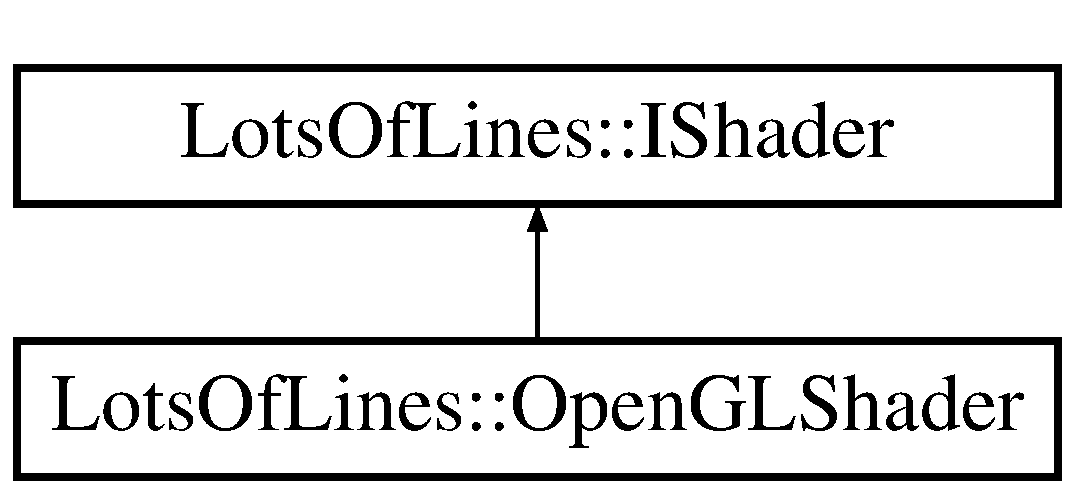
\includegraphics[height=2.000000cm]{class_lots_of_lines_1_1_i_shader}
\end{center}
\end{figure}
\subsection*{Public Member Functions}
\begin{DoxyCompactItemize}
\item 
virtual bool \hyperlink{class_lots_of_lines_1_1_i_shader_ae36eff82b2940ff5d16b938bb67edd2b}{compile} (const char $\ast$vertex\+Shader\+Src, const char $\ast$fragment\+Shader\+Src)=0\hypertarget{class_lots_of_lines_1_1_i_shader_ae36eff82b2940ff5d16b938bb67edd2b}{}\label{class_lots_of_lines_1_1_i_shader_ae36eff82b2940ff5d16b938bb67edd2b}

\begin{DoxyCompactList}\small\item\em Compile a shader program from source code. \end{DoxyCompactList}\end{DoxyCompactItemize}


The documentation for this class was generated from the following file\+:\begin{DoxyCompactItemize}
\item 
D\+:/\+School/\+C\+W\+U/\+C\+S 481/\+Lots-\/of-\/\+Lines/source/\+Rendering\+System/I\+Shader.\+hpp\end{DoxyCompactItemize}

\hypertarget{class_lots_of_lines_1_1_data_set_1_1_iterator}{}\section{Lots\+Of\+Lines\+:\+:Data\+Set\+:\+:Iterator Class Reference}
\label{class_lots_of_lines_1_1_data_set_1_1_iterator}\index{Lots\+Of\+Lines\+::\+Data\+Set\+::\+Iterator@{Lots\+Of\+Lines\+::\+Data\+Set\+::\+Iterator}}


\hyperlink{class_lots_of_lines_1_1_data_set_1_1_iterator}{Iterator} class for traversing the dataset easier.  




{\ttfamily \#include $<$Data\+Set.\+hpp$>$}

\subsection*{Public Member Functions}
\begin{DoxyCompactItemize}
\item 
\hyperlink{class_lots_of_lines_1_1_data_set_1_1_iterator}{Iterator} \& {\bfseries operator++} (int)\hypertarget{class_lots_of_lines_1_1_data_set_1_1_iterator_a27ecd81fbc84de916319afb95b9397fc}{}\label{class_lots_of_lines_1_1_data_set_1_1_iterator_a27ecd81fbc84de916319afb95b9397fc}

\item 
bool \hyperlink{class_lots_of_lines_1_1_data_set_1_1_iterator_a560719900b7c83fa0863061614b3d38b}{has\+Next} () const 
\item 
const Vector \& \hyperlink{class_lots_of_lines_1_1_data_set_1_1_iterator_a986cb3be36d6d3dd3dc59ca1db5f7fb5}{vector} ()
\item 
unsigned int \hyperlink{class_lots_of_lines_1_1_data_set_1_1_iterator_ac76ed57d62efaecfc1baf1c3b831eae5}{class\+Index} () const 
\item 
unsigned int \hyperlink{class_lots_of_lines_1_1_data_set_1_1_iterator_a309c1a1a53f80c764e4d77f15ba7c171}{line\+Index} () const 
\end{DoxyCompactItemize}
\subsection*{Protected Member Functions}
\begin{DoxyCompactItemize}
\item 
{\bfseries Iterator} (const \hyperlink{class_lots_of_lines_1_1_data_set}{Data\+Set} $\ast$data\+Set)\hypertarget{class_lots_of_lines_1_1_data_set_1_1_iterator_ab697d4871ed39b319956e903104c90a3}{}\label{class_lots_of_lines_1_1_data_set_1_1_iterator_ab697d4871ed39b319956e903104c90a3}

\end{DoxyCompactItemize}
\subsection*{Protected Attributes}
\begin{DoxyCompactItemize}
\item 
const \hyperlink{class_lots_of_lines_1_1_data_set}{Data\+Set} $\ast$ {\bfseries m\+\_\+data\+Set}\hypertarget{class_lots_of_lines_1_1_data_set_1_1_iterator_ada58776aa7f1f0ff1d1d217e05b3dc4c}{}\label{class_lots_of_lines_1_1_data_set_1_1_iterator_ada58776aa7f1f0ff1d1d217e05b3dc4c}

\item 
unsigned int {\bfseries m\+\_\+vector\+Idx}\hypertarget{class_lots_of_lines_1_1_data_set_1_1_iterator_ae0c142ecd8398e46ef10625acdbe410d}{}\label{class_lots_of_lines_1_1_data_set_1_1_iterator_ae0c142ecd8398e46ef10625acdbe410d}

\end{DoxyCompactItemize}
\subsection*{Friends}
\begin{DoxyCompactItemize}
\item 
class {\bfseries Data\+Set}\hypertarget{class_lots_of_lines_1_1_data_set_1_1_iterator_aef648af6c56fa8ee0738c93629e725dc}{}\label{class_lots_of_lines_1_1_data_set_1_1_iterator_aef648af6c56fa8ee0738c93629e725dc}

\end{DoxyCompactItemize}


\subsection{Detailed Description}
\hyperlink{class_lots_of_lines_1_1_data_set_1_1_iterator}{Iterator} class for traversing the dataset easier. 

\subsection{Member Function Documentation}
\index{Lots\+Of\+Lines\+::\+Data\+Set\+::\+Iterator@{Lots\+Of\+Lines\+::\+Data\+Set\+::\+Iterator}!class\+Index@{class\+Index}}
\index{class\+Index@{class\+Index}!Lots\+Of\+Lines\+::\+Data\+Set\+::\+Iterator@{Lots\+Of\+Lines\+::\+Data\+Set\+::\+Iterator}}
\subsubsection[{\texorpdfstring{class\+Index() const }{classIndex() const }}]{\setlength{\rightskip}{0pt plus 5cm}unsigned int Data\+Set\+::\+Iterator\+::class\+Index (
\begin{DoxyParamCaption}
{}
\end{DoxyParamCaption}
) const}\hypertarget{class_lots_of_lines_1_1_data_set_1_1_iterator_ac76ed57d62efaecfc1baf1c3b831eae5}{}\label{class_lots_of_lines_1_1_data_set_1_1_iterator_ac76ed57d62efaecfc1baf1c3b831eae5}
\begin{DoxyReturn}{Returns}
The class index of the current vector. 
\end{DoxyReturn}
\index{Lots\+Of\+Lines\+::\+Data\+Set\+::\+Iterator@{Lots\+Of\+Lines\+::\+Data\+Set\+::\+Iterator}!has\+Next@{has\+Next}}
\index{has\+Next@{has\+Next}!Lots\+Of\+Lines\+::\+Data\+Set\+::\+Iterator@{Lots\+Of\+Lines\+::\+Data\+Set\+::\+Iterator}}
\subsubsection[{\texorpdfstring{has\+Next() const }{hasNext() const }}]{\setlength{\rightskip}{0pt plus 5cm}bool Data\+Set\+::\+Iterator\+::has\+Next (
\begin{DoxyParamCaption}
{}
\end{DoxyParamCaption}
) const}\hypertarget{class_lots_of_lines_1_1_data_set_1_1_iterator_a560719900b7c83fa0863061614b3d38b}{}\label{class_lots_of_lines_1_1_data_set_1_1_iterator_a560719900b7c83fa0863061614b3d38b}
\begin{DoxyReturn}{Returns}
True if there\textquotesingle{}s a next vector available, false if the end has been reached. 
\end{DoxyReturn}
\index{Lots\+Of\+Lines\+::\+Data\+Set\+::\+Iterator@{Lots\+Of\+Lines\+::\+Data\+Set\+::\+Iterator}!line\+Index@{line\+Index}}
\index{line\+Index@{line\+Index}!Lots\+Of\+Lines\+::\+Data\+Set\+::\+Iterator@{Lots\+Of\+Lines\+::\+Data\+Set\+::\+Iterator}}
\subsubsection[{\texorpdfstring{line\+Index() const }{lineIndex() const }}]{\setlength{\rightskip}{0pt plus 5cm}unsigned int Data\+Set\+::\+Iterator\+::line\+Index (
\begin{DoxyParamCaption}
{}
\end{DoxyParamCaption}
) const}\hypertarget{class_lots_of_lines_1_1_data_set_1_1_iterator_a309c1a1a53f80c764e4d77f15ba7c171}{}\label{class_lots_of_lines_1_1_data_set_1_1_iterator_a309c1a1a53f80c764e4d77f15ba7c171}
\begin{DoxyReturn}{Returns}
The index of the current vector. 
\end{DoxyReturn}
\index{Lots\+Of\+Lines\+::\+Data\+Set\+::\+Iterator@{Lots\+Of\+Lines\+::\+Data\+Set\+::\+Iterator}!vector@{vector}}
\index{vector@{vector}!Lots\+Of\+Lines\+::\+Data\+Set\+::\+Iterator@{Lots\+Of\+Lines\+::\+Data\+Set\+::\+Iterator}}
\subsubsection[{\texorpdfstring{vector()}{vector()}}]{\setlength{\rightskip}{0pt plus 5cm}const Vector \& Data\+Set\+::\+Iterator\+::vector (
\begin{DoxyParamCaption}
{}
\end{DoxyParamCaption}
)}\hypertarget{class_lots_of_lines_1_1_data_set_1_1_iterator_a986cb3be36d6d3dd3dc59ca1db5f7fb5}{}\label{class_lots_of_lines_1_1_data_set_1_1_iterator_a986cb3be36d6d3dd3dc59ca1db5f7fb5}
\begin{DoxyReturn}{Returns}
Vector in the \hyperlink{class_lots_of_lines_1_1_data_set}{Data\+Set}, or nullptr if the end has been reached. 
\end{DoxyReturn}


The documentation for this class was generated from the following files\+:\begin{DoxyCompactItemize}
\item 
D\+:/\+School/\+C\+W\+U/\+C\+S 481/\+Lots-\/of-\/\+Lines/source/\+Data\+Model/Data\+Set.\+hpp\item 
D\+:/\+School/\+C\+W\+U/\+C\+S 481/\+Lots-\/of-\/\+Lines/source/\+Data\+Model/Data\+Set.\+cpp\end{DoxyCompactItemize}

\hypertarget{class_lots_of_lines_1_1_i_vertex_buffer_object}{}\section{Lots\+Of\+Lines\+:\+:I\+Vertex\+Buffer\+Object Class Reference}
\label{class_lots_of_lines_1_1_i_vertex_buffer_object}\index{Lots\+Of\+Lines\+::\+I\+Vertex\+Buffer\+Object@{Lots\+Of\+Lines\+::\+I\+Vertex\+Buffer\+Object}}


Interface for creating vertex/index buffer (Open\+GL V\+BO) \hyperlink{struct_lots_of_lines_1_1_vertex}{Vertex} Buffer Objects should only be constructed through the \hyperlink{class_lots_of_lines_1_1_i_renderer}{I\+Renderer} interface.  




{\ttfamily \#include $<$I\+Vertex\+Buffer\+Object.\+hpp$>$}

Inheritance diagram for Lots\+Of\+Lines\+:\+:I\+Vertex\+Buffer\+Object\+:\begin{figure}[H]
\begin{center}
\leavevmode
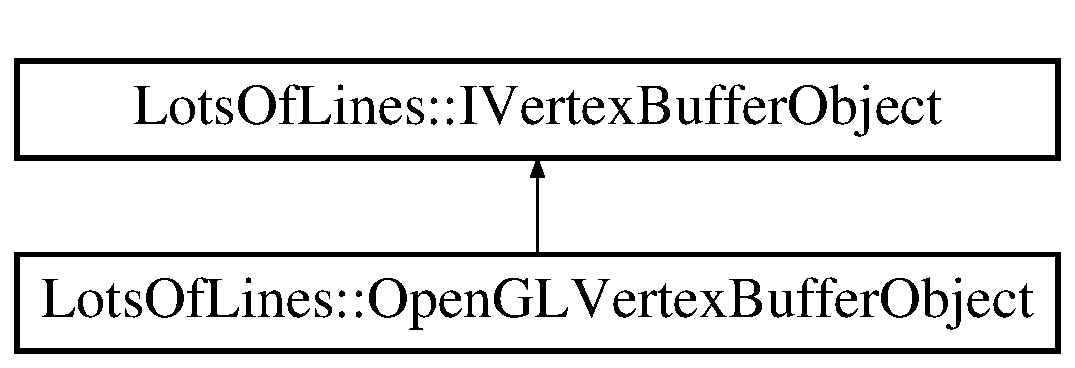
\includegraphics[height=2.000000cm]{class_lots_of_lines_1_1_i_vertex_buffer_object}
\end{center}
\end{figure}
\subsection*{Public Member Functions}
\begin{DoxyCompactItemize}
\item 
virtual \hyperlink{struct_lots_of_lines_1_1_vertex}{Vertex} $\ast$ \hyperlink{class_lots_of_lines_1_1_i_vertex_buffer_object_ae367bf3f773738ffb1bf6957dba1cc13}{map\+Vertices} (bool read\+Only=false)=0
\begin{DoxyCompactList}\small\item\em Map the vertex buffer for access. \end{DoxyCompactList}\item 
virtual void \hyperlink{class_lots_of_lines_1_1_i_vertex_buffer_object_afc26bc993026fa665f2514f07193468c}{unmap\+Vertices} ()=0\hypertarget{class_lots_of_lines_1_1_i_vertex_buffer_object_afc26bc993026fa665f2514f07193468c}{}\label{class_lots_of_lines_1_1_i_vertex_buffer_object_afc26bc993026fa665f2514f07193468c}

\begin{DoxyCompactList}\small\item\em Unmap (unlock) the vertex buffer after accessing it. \end{DoxyCompactList}\item 
virtual unsigned int $\ast$ \hyperlink{class_lots_of_lines_1_1_i_vertex_buffer_object_a8820943ddcb998bccb03a9769611218b}{map\+Indices} ()=0
\begin{DoxyCompactList}\small\item\em Map the index buffer for access. \end{DoxyCompactList}\item 
virtual void \hyperlink{class_lots_of_lines_1_1_i_vertex_buffer_object_ad9d74ca76d582e530150c93a95e71595}{unmap\+Indices} ()=0\hypertarget{class_lots_of_lines_1_1_i_vertex_buffer_object_ad9d74ca76d582e530150c93a95e71595}{}\label{class_lots_of_lines_1_1_i_vertex_buffer_object_ad9d74ca76d582e530150c93a95e71595}

\begin{DoxyCompactList}\small\item\em Unmap (unlock) the index buffer after accessing it. \end{DoxyCompactList}\item 
virtual unsigned int {\bfseries vertex\+Count} () const  =0\hypertarget{class_lots_of_lines_1_1_i_vertex_buffer_object_a3aaaf9b75c1d85be76ea9991bf258776}{}\label{class_lots_of_lines_1_1_i_vertex_buffer_object_a3aaaf9b75c1d85be76ea9991bf258776}

\item 
virtual unsigned int {\bfseries index\+Count} () const  =0\hypertarget{class_lots_of_lines_1_1_i_vertex_buffer_object_a565dc4ffbdd130359cc27465e1e52176}{}\label{class_lots_of_lines_1_1_i_vertex_buffer_object_a565dc4ffbdd130359cc27465e1e52176}

\end{DoxyCompactItemize}


\subsection{Detailed Description}
Interface for creating vertex/index buffer (Open\+GL V\+BO) \hyperlink{struct_lots_of_lines_1_1_vertex}{Vertex} Buffer Objects should only be constructed through the \hyperlink{class_lots_of_lines_1_1_i_renderer}{I\+Renderer} interface. 

\subsection{Member Function Documentation}
\index{Lots\+Of\+Lines\+::\+I\+Vertex\+Buffer\+Object@{Lots\+Of\+Lines\+::\+I\+Vertex\+Buffer\+Object}!map\+Indices@{map\+Indices}}
\index{map\+Indices@{map\+Indices}!Lots\+Of\+Lines\+::\+I\+Vertex\+Buffer\+Object@{Lots\+Of\+Lines\+::\+I\+Vertex\+Buffer\+Object}}
\subsubsection[{\texorpdfstring{map\+Indices()=0}{mapIndices()=0}}]{\setlength{\rightskip}{0pt plus 5cm}virtual unsigned int$\ast$ Lots\+Of\+Lines\+::\+I\+Vertex\+Buffer\+Object\+::map\+Indices (
\begin{DoxyParamCaption}
{}
\end{DoxyParamCaption}
)\hspace{0.3cm}{\ttfamily [pure virtual]}}\hypertarget{class_lots_of_lines_1_1_i_vertex_buffer_object_a8820943ddcb998bccb03a9769611218b}{}\label{class_lots_of_lines_1_1_i_vertex_buffer_object_a8820943ddcb998bccb03a9769611218b}


Map the index buffer for access. 

\begin{DoxyReturn}{Returns}
A pointer to the index buffer\textquotesingle{}s data, or N\+U\+LL if the buffer couldn\textquotesingle{}t be mapped. 
\end{DoxyReturn}


Implemented in \hyperlink{class_lots_of_lines_1_1_open_g_l_vertex_buffer_object_a59c71c761341ca1732b5816bdfe6d239}{Lots\+Of\+Lines\+::\+Open\+G\+L\+Vertex\+Buffer\+Object}.

\index{Lots\+Of\+Lines\+::\+I\+Vertex\+Buffer\+Object@{Lots\+Of\+Lines\+::\+I\+Vertex\+Buffer\+Object}!map\+Vertices@{map\+Vertices}}
\index{map\+Vertices@{map\+Vertices}!Lots\+Of\+Lines\+::\+I\+Vertex\+Buffer\+Object@{Lots\+Of\+Lines\+::\+I\+Vertex\+Buffer\+Object}}
\subsubsection[{\texorpdfstring{map\+Vertices(bool read\+Only=false)=0}{mapVertices(bool readOnly=false)=0}}]{\setlength{\rightskip}{0pt plus 5cm}virtual {\bf Vertex}$\ast$ Lots\+Of\+Lines\+::\+I\+Vertex\+Buffer\+Object\+::map\+Vertices (
\begin{DoxyParamCaption}
\item[{bool}]{read\+Only = {\ttfamily false}}
\end{DoxyParamCaption}
)\hspace{0.3cm}{\ttfamily [pure virtual]}}\hypertarget{class_lots_of_lines_1_1_i_vertex_buffer_object_ae367bf3f773738ffb1bf6957dba1cc13}{}\label{class_lots_of_lines_1_1_i_vertex_buffer_object_ae367bf3f773738ffb1bf6957dba1cc13}


Map the vertex buffer for access. 

\begin{DoxyReturn}{Returns}
A pointer to the vertex buffer\textquotesingle{}s data, or N\+U\+LL if the buffer couldn\textquotesingle{}t be mapped. 
\end{DoxyReturn}


Implemented in \hyperlink{class_lots_of_lines_1_1_open_g_l_vertex_buffer_object_a842ae500f862c5fb011ce1fa93478236}{Lots\+Of\+Lines\+::\+Open\+G\+L\+Vertex\+Buffer\+Object}.



The documentation for this class was generated from the following file\+:\begin{DoxyCompactItemize}
\item 
D\+:/\+School/\+C\+W\+U/\+C\+S 481/\+Lots-\/of-\/\+Lines/source/\+Rendering\+System/I\+Vertex\+Buffer\+Object.\+hpp\end{DoxyCompactItemize}

\hypertarget{class_lots_of_lines_1_1_i_visualization_method}{}\section{Lots\+Of\+Lines\+:\+:I\+Visualization\+Method Class Reference}
\label{class_lots_of_lines_1_1_i_visualization_method}\index{Lots\+Of\+Lines\+::\+I\+Visualization\+Method@{Lots\+Of\+Lines\+::\+I\+Visualization\+Method}}


Visualization method interface for generating vertex buffers based on a dataset.  




{\ttfamily \#include $<$I\+Visualization\+Method.\+hpp$>$}

Inheritance diagram for Lots\+Of\+Lines\+:\+:I\+Visualization\+Method\+:\begin{figure}[H]
\begin{center}
\leavevmode
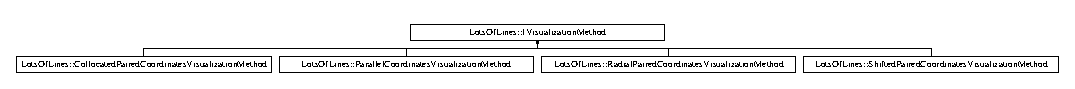
\includegraphics[height=0.754717cm]{class_lots_of_lines_1_1_i_visualization_method}
\end{center}
\end{figure}
\subsection*{Public Member Functions}
\begin{DoxyCompactItemize}
\item 
virtual E\+\_\+\+V\+I\+S\+U\+A\+L\+I\+Z\+A\+T\+I\+O\+N\+\_\+\+T\+Y\+PE \hyperlink{class_lots_of_lines_1_1_i_visualization_method_a79b6c5d987437bcc7204c4e63aba7c31}{get\+Type} ()=0
\item 
virtual std\+::string \hyperlink{class_lots_of_lines_1_1_i_visualization_method_adbf8ab4dff252bbc3491e4acbebd0d28}{get\+Type\+Name} ()=0
\item 
virtual bool \hyperlink{class_lots_of_lines_1_1_i_visualization_method_ac31b5ad80f94fdfcf424a75b6afe27ea}{generate\+V\+BO} (const std\+::shared\+\_\+ptr$<$ const \hyperlink{class_lots_of_lines_1_1_data_set}{Data\+Set} $>$ data\+Set, std\+::vector$<$ \hyperlink{struct_lots_of_lines_1_1_vertex}{Vertex} $>$ \&vertices\+Out, std\+::vector$<$ unsigned int $>$ \&indices\+Out, \hyperlink{class_lots_of_lines_1_1_rendering_system}{Rendering\+System} $\ast$driver, const \hyperlink{class_lots_of_lines_1_1_visualization_options}{Visualization\+Options} \&options=\hyperlink{class_lots_of_lines_1_1_visualization_options}{Visualization\+Options}())=0\hypertarget{class_lots_of_lines_1_1_i_visualization_method_ac31b5ad80f94fdfcf424a75b6afe27ea}{}\label{class_lots_of_lines_1_1_i_visualization_method_ac31b5ad80f94fdfcf424a75b6afe27ea}

\begin{DoxyCompactList}\small\item\em Generate a vertex buffer for the visualization. \end{DoxyCompactList}\item 
virtual void \hyperlink{class_lots_of_lines_1_1_i_visualization_method_ac03a0f363501f36fec7cecdace77db0d}{pre\+Draw} (\hyperlink{class_lots_of_lines_1_1_rendering_system}{Rendering\+System} $\ast$)\hypertarget{class_lots_of_lines_1_1_i_visualization_method_ac03a0f363501f36fec7cecdace77db0d}{}\label{class_lots_of_lines_1_1_i_visualization_method_ac03a0f363501f36fec7cecdace77db0d}

\begin{DoxyCompactList}\small\item\em Draw axis lines and other extra features of the visualization method. \end{DoxyCompactList}\item 
virtual void \hyperlink{class_lots_of_lines_1_1_i_visualization_method_a4e79488141ff0b4ec79dc11c72184b2a}{get\+Navigation\+Options} (\hyperlink{struct_lots_of_lines_1_1_navigation_options}{Navigation\+Options} \&options\+Out)=0\hypertarget{class_lots_of_lines_1_1_i_visualization_method_a4e79488141ff0b4ec79dc11c72184b2a}{}\label{class_lots_of_lines_1_1_i_visualization_method_a4e79488141ff0b4ec79dc11c72184b2a}

\begin{DoxyCompactList}\small\item\em Should return the navigation options for the rendering method (X scroll lock, etc) \end{DoxyCompactList}\item 
virtual void \hyperlink{class_lots_of_lines_1_1_i_visualization_method_a96b1bc601ba7769a1aaed16e0d55f641}{get\+Default\+Options} (\hyperlink{class_lots_of_lines_1_1_visualization_options}{Visualization\+Options} \&)\hypertarget{class_lots_of_lines_1_1_i_visualization_method_a96b1bc601ba7769a1aaed16e0d55f641}{}\label{class_lots_of_lines_1_1_i_visualization_method_a96b1bc601ba7769a1aaed16e0d55f641}

\begin{DoxyCompactList}\small\item\em Should fill an empty \hyperlink{class_lots_of_lines_1_1_visualization_options}{Visualization\+Options} object with the default options to use for the visualization method. This method will be called once when the visualization method is loaded in order to generate fields for the UI system. \end{DoxyCompactList}\end{DoxyCompactItemize}


\subsection{Detailed Description}
Visualization method interface for generating vertex buffers based on a dataset. 

\subsection{Member Function Documentation}
\index{Lots\+Of\+Lines\+::\+I\+Visualization\+Method@{Lots\+Of\+Lines\+::\+I\+Visualization\+Method}!get\+Type@{get\+Type}}
\index{get\+Type@{get\+Type}!Lots\+Of\+Lines\+::\+I\+Visualization\+Method@{Lots\+Of\+Lines\+::\+I\+Visualization\+Method}}
\subsubsection[{\texorpdfstring{get\+Type()=0}{getType()=0}}]{\setlength{\rightskip}{0pt plus 5cm}virtual E\+\_\+\+V\+I\+S\+U\+A\+L\+I\+Z\+A\+T\+I\+O\+N\+\_\+\+T\+Y\+PE Lots\+Of\+Lines\+::\+I\+Visualization\+Method\+::get\+Type (
\begin{DoxyParamCaption}
{}
\end{DoxyParamCaption}
)\hspace{0.3cm}{\ttfamily [pure virtual]}}\hypertarget{class_lots_of_lines_1_1_i_visualization_method_a79b6c5d987437bcc7204c4e63aba7c31}{}\label{class_lots_of_lines_1_1_i_visualization_method_a79b6c5d987437bcc7204c4e63aba7c31}
\begin{DoxyReturn}{Returns}
The enum type of the visualization method. 
\end{DoxyReturn}
\index{Lots\+Of\+Lines\+::\+I\+Visualization\+Method@{Lots\+Of\+Lines\+::\+I\+Visualization\+Method}!get\+Type\+Name@{get\+Type\+Name}}
\index{get\+Type\+Name@{get\+Type\+Name}!Lots\+Of\+Lines\+::\+I\+Visualization\+Method@{Lots\+Of\+Lines\+::\+I\+Visualization\+Method}}
\subsubsection[{\texorpdfstring{get\+Type\+Name()=0}{getTypeName()=0}}]{\setlength{\rightskip}{0pt plus 5cm}virtual std\+::string Lots\+Of\+Lines\+::\+I\+Visualization\+Method\+::get\+Type\+Name (
\begin{DoxyParamCaption}
{}
\end{DoxyParamCaption}
)\hspace{0.3cm}{\ttfamily [pure virtual]}}\hypertarget{class_lots_of_lines_1_1_i_visualization_method_adbf8ab4dff252bbc3491e4acbebd0d28}{}\label{class_lots_of_lines_1_1_i_visualization_method_adbf8ab4dff252bbc3491e4acbebd0d28}
\begin{DoxyReturn}{Returns}
The string type name of the visualization method. 
\end{DoxyReturn}


The documentation for this class was generated from the following file\+:\begin{DoxyCompactItemize}
\item 
D\+:/\+School/\+C\+W\+U/\+C\+S 481/\+Lots-\/of-\/\+Lines/source/\+Rendering\+System/I\+Visualization\+Method.\+hpp\end{DoxyCompactItemize}

\hypertarget{class_load_data_dialog}{}\section{Load\+Data\+Dialog Class Reference}
\label{class_load_data_dialog}\index{Load\+Data\+Dialog@{Load\+Data\+Dialog}}
Inheritance diagram for Load\+Data\+Dialog\+:\begin{figure}[H]
\begin{center}
\leavevmode
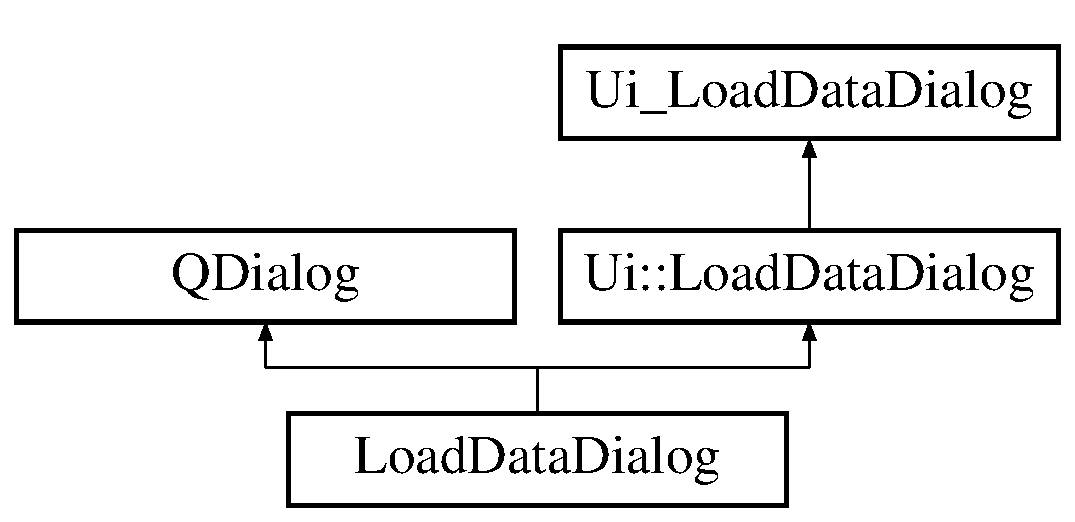
\includegraphics[height=3.000000cm]{class_load_data_dialog}
\end{center}
\end{figure}
\subsection*{Public Slots}
\begin{DoxyCompactItemize}
\item 
void {\bfseries custom\+Class\+Checked} (int state)\hypertarget{class_load_data_dialog_a16696e5f01c2935a4a30094069914f82}{}\label{class_load_data_dialog_a16696e5f01c2935a4a30094069914f82}

\end{DoxyCompactItemize}
\subsection*{Public Member Functions}
\begin{DoxyCompactItemize}
\item 
{\bfseries Load\+Data\+Dialog} (Q\+Widget $\ast$parent, const Q\+String \&file\+Path)\hypertarget{class_load_data_dialog_aff71f0e7a55c65550aa7247b5378da34}{}\label{class_load_data_dialog_aff71f0e7a55c65550aa7247b5378da34}

\item 
\hyperlink{struct_lots_of_lines_1_1_load_options}{Lots\+Of\+Lines\+::\+Load\+Options} {\bfseries get\+Load\+Options} ()\hypertarget{class_load_data_dialog_a520548008761823248425b849ec9eae2}{}\label{class_load_data_dialog_a520548008761823248425b849ec9eae2}

\end{DoxyCompactItemize}
\subsection*{Additional Inherited Members}


The documentation for this class was generated from the following files\+:\begin{DoxyCompactItemize}
\item 
D\+:/\+School/\+C\+W\+U/\+C\+S 481/\+Lots-\/of-\/\+Lines/source/Load\+Data\+Dialog.\+h\item 
D\+:/\+School/\+C\+W\+U/\+C\+S 481/\+Lots-\/of-\/\+Lines/source/Load\+Data\+Dialog.\+cpp\end{DoxyCompactItemize}

\hypertarget{class_ui_1_1_load_data_dialog}{}\section{Ui\+:\+:Load\+Data\+Dialog Class Reference}
\label{class_ui_1_1_load_data_dialog}\index{Ui\+::\+Load\+Data\+Dialog@{Ui\+::\+Load\+Data\+Dialog}}
Inheritance diagram for Ui\+:\+:Load\+Data\+Dialog\+:\begin{figure}[H]
\begin{center}
\leavevmode
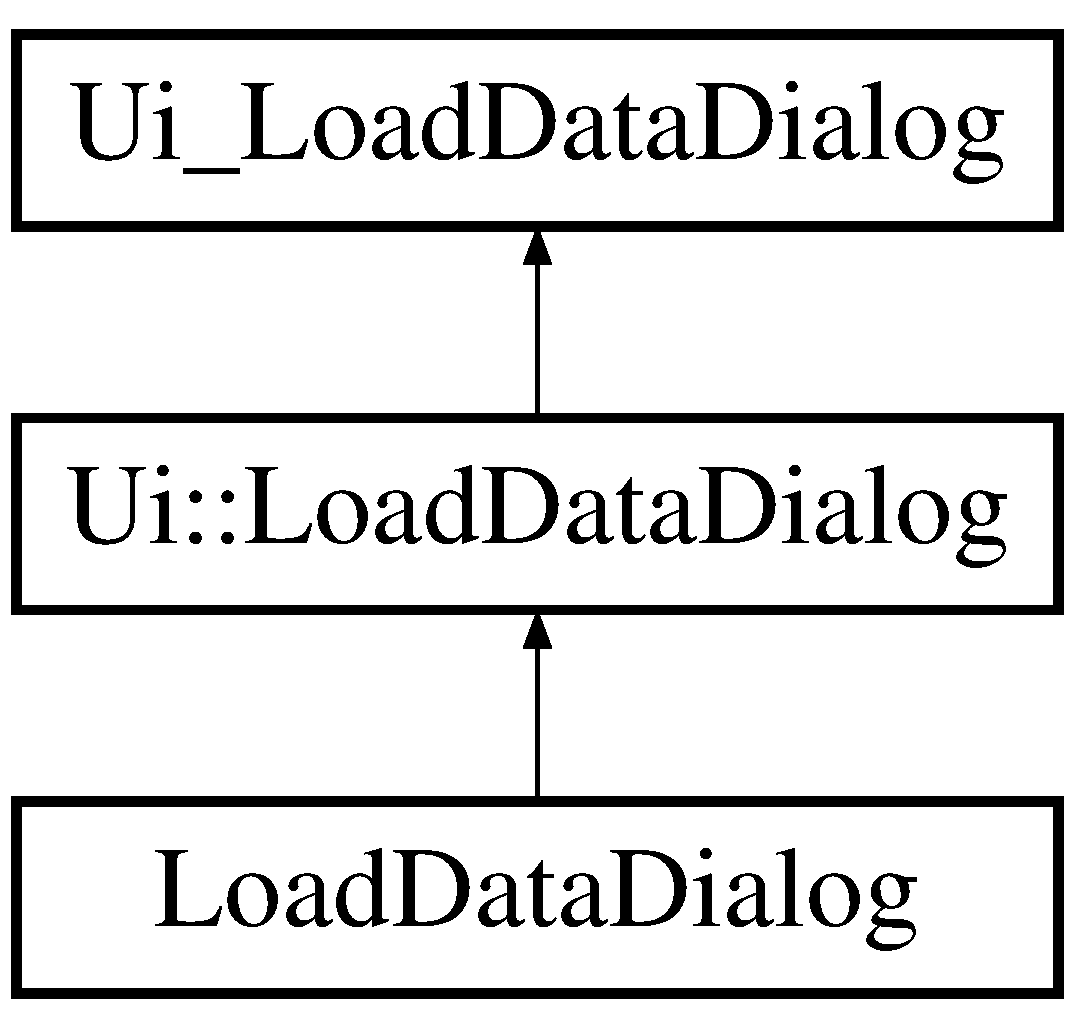
\includegraphics[height=3.000000cm]{class_ui_1_1_load_data_dialog}
\end{center}
\end{figure}
\subsection*{Additional Inherited Members}


The documentation for this class was generated from the following file\+:\begin{DoxyCompactItemize}
\item 
D\+:/\+School/\+C\+W\+U/\+C\+S 481/\+Lots-\/of-\/\+Lines/source/\+Generated\+Files/ui\+\_\+\+Load\+Data\+Dialog.\+h\end{DoxyCompactItemize}

\hypertarget{class_loading_worker}{}\section{Loading\+Worker Class Reference}
\label{class_loading_worker}\index{Loading\+Worker@{Loading\+Worker}}
Inheritance diagram for Loading\+Worker\+:\begin{figure}[H]
\begin{center}
\leavevmode
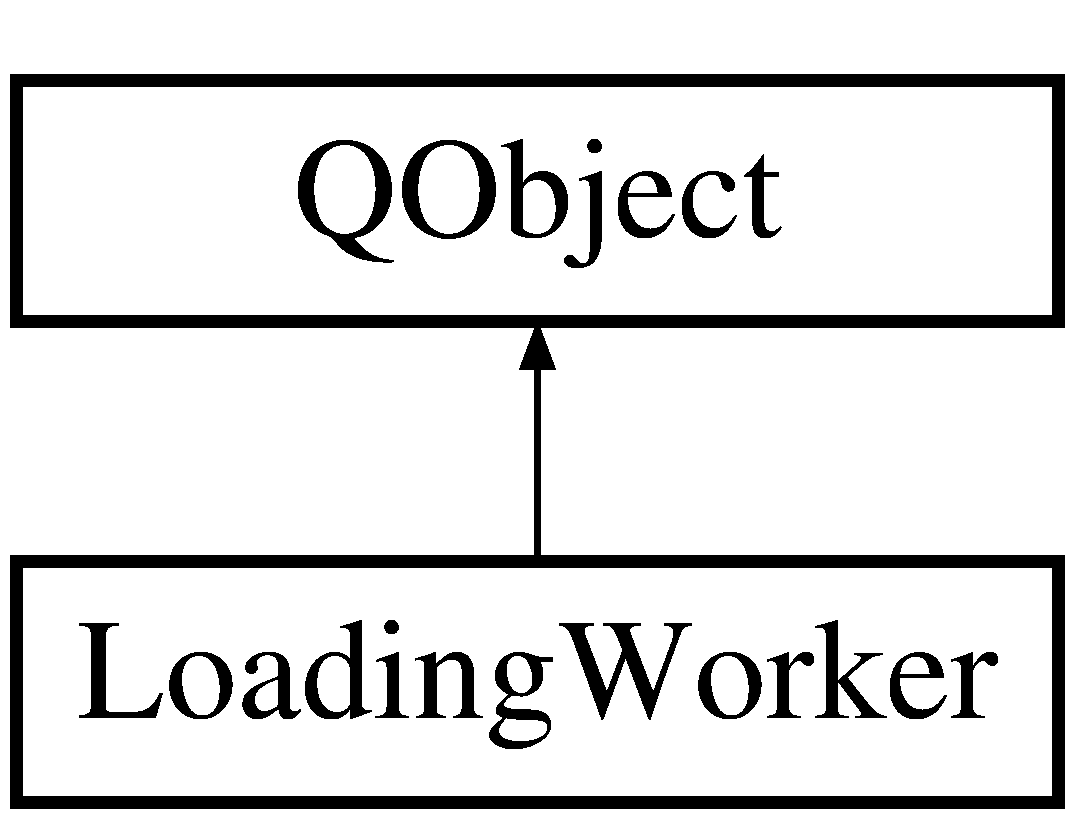
\includegraphics[height=2.000000cm]{class_loading_worker}
\end{center}
\end{figure}
\subsection*{Public Slots}
\begin{DoxyCompactItemize}
\item 
void {\bfseries update\+Dataset} (const Q\+String \&path, const \hyperlink{struct_lots_of_lines_1_1_load_options}{Lots\+Of\+Lines\+::\+Load\+Options} \&options)\hypertarget{class_loading_worker_ab73de964995a1e14a0e58829b0a8c23c}{}\label{class_loading_worker_ab73de964995a1e14a0e58829b0a8c23c}

\end{DoxyCompactItemize}
\subsection*{Signals}
\begin{DoxyCompactItemize}
\item 
void {\bfseries dataset\+Updated} (std\+::shared\+\_\+ptr$<$ \hyperlink{class_lots_of_lines_1_1_data_set}{Lots\+Of\+Lines\+::\+Data\+Set} $>$)\hypertarget{class_loading_worker_ae10e9b2b8b006cc6ca04e5f9f78ff729}{}\label{class_loading_worker_ae10e9b2b8b006cc6ca04e5f9f78ff729}

\end{DoxyCompactItemize}
\subsection*{Public Member Functions}
\begin{DoxyCompactItemize}
\item 
{\bfseries Loading\+Worker} (\hyperlink{class_lots_of_lines_1_1_progress_message}{Lots\+Of\+Lines\+::\+Progress\+Message} $\ast$)\hypertarget{class_loading_worker_a3f5b1820e6770cc3d981360d730cd7dc}{}\label{class_loading_worker_a3f5b1820e6770cc3d981360d730cd7dc}

\item 
std\+::shared\+\_\+ptr$<$ \hyperlink{class_lots_of_lines_1_1_data_set}{Lots\+Of\+Lines\+::\+Data\+Set} $>$ {\bfseries load\+Data} (const Q\+String \&path, const \hyperlink{struct_lots_of_lines_1_1_load_options}{Lots\+Of\+Lines\+::\+Load\+Options} \&options)\hypertarget{class_loading_worker_abbabae8666e6f2f8cd5ec90d172b414b}{}\label{class_loading_worker_abbabae8666e6f2f8cd5ec90d172b414b}

\end{DoxyCompactItemize}
\subsection*{Protected Attributes}
\begin{DoxyCompactItemize}
\item 
\hyperlink{class_lots_of_lines_1_1_data_model}{Lots\+Of\+Lines\+::\+Data\+Model} {\bfseries m\+\_\+data\+Model}\hypertarget{class_loading_worker_a1688b4d70f0007faafdb59b3f9ba79b6}{}\label{class_loading_worker_a1688b4d70f0007faafdb59b3f9ba79b6}

\item 
\hyperlink{class_lots_of_lines_1_1_progress_message}{Lots\+Of\+Lines\+::\+Progress\+Message} $\ast$ {\bfseries m\+\_\+progress}\hypertarget{class_loading_worker_a2f4ce82052cbcc0ba982e8ff6d2cd709}{}\label{class_loading_worker_a2f4ce82052cbcc0ba982e8ff6d2cd709}

\end{DoxyCompactItemize}


The documentation for this class was generated from the following files\+:\begin{DoxyCompactItemize}
\item 
D\+:/\+School/\+C\+W\+U/\+C\+S 481/\+Lots-\/of-\/\+Lines/source/Loading\+Worker.\+h\item 
D\+:/\+School/\+C\+W\+U/\+C\+S 481/\+Lots-\/of-\/\+Lines/source/Loading\+Worker.\+cpp\end{DoxyCompactItemize}

\hypertarget{struct_lots_of_lines_1_1_load_options}{}\section{Lots\+Of\+Lines\+:\+:Load\+Options Struct Reference}
\label{struct_lots_of_lines_1_1_load_options}\index{Lots\+Of\+Lines\+::\+Load\+Options@{Lots\+Of\+Lines\+::\+Load\+Options}}
\subsection*{Public Attributes}
\begin{DoxyCompactItemize}
\item 
E\+\_\+\+D\+A\+T\+A\+\_\+\+N\+O\+R\+M\+A\+L\+I\+Z\+A\+T\+I\+O\+N\+\_\+\+M\+O\+DE \hyperlink{struct_lots_of_lines_1_1_load_options_aaa84493d2ccff03e0c44c604418f45d4}{data\+Normalization\+Mode}\hypertarget{struct_lots_of_lines_1_1_load_options_aaa84493d2ccff03e0c44c604418f45d4}{}\label{struct_lots_of_lines_1_1_load_options_aaa84493d2ccff03e0c44c604418f45d4}

\begin{DoxyCompactList}\small\item\em Mode of normalization to use after loading. \end{DoxyCompactList}\item 
bool \hyperlink{struct_lots_of_lines_1_1_load_options_aebc8f69db09dab1ffe878a758adf2546}{custom\+Class\+Column}\hypertarget{struct_lots_of_lines_1_1_load_options_aebc8f69db09dab1ffe878a758adf2546}{}\label{struct_lots_of_lines_1_1_load_options_aebc8f69db09dab1ffe878a758adf2546}

\begin{DoxyCompactList}\small\item\em Whether to override the class column, or to just use the last one. \end{DoxyCompactList}\item 
unsigned int \hyperlink{struct_lots_of_lines_1_1_load_options_a67ed8b21547e5d38e0c3ecebca3afc7e}{class\+Column}\hypertarget{struct_lots_of_lines_1_1_load_options_a67ed8b21547e5d38e0c3ecebca3afc7e}{}\label{struct_lots_of_lines_1_1_load_options_a67ed8b21547e5d38e0c3ecebca3afc7e}

\begin{DoxyCompactList}\small\item\em Column to use as data class label. \end{DoxyCompactList}\item 
std\+::vector$<$ unsigned int $>$ \hyperlink{struct_lots_of_lines_1_1_load_options_aa31ca1ba223ee074bf175594e66e6f1f}{ignore\+Columns}\hypertarget{struct_lots_of_lines_1_1_load_options_aa31ca1ba223ee074bf175594e66e6f1f}{}\label{struct_lots_of_lines_1_1_load_options_aa31ca1ba223ee074bf175594e66e6f1f}

\begin{DoxyCompactList}\small\item\em Array of columns to ignore when loading the data. \end{DoxyCompactList}\end{DoxyCompactItemize}
\subsection*{Static Public Attributes}
\begin{DoxyCompactItemize}
\item 
static const \hyperlink{struct_lots_of_lines_1_1_load_options}{Load\+Options} {\bfseries default} = \hyperlink{struct_lots_of_lines_1_1_load_options}{Load\+Options}()\hypertarget{struct_lots_of_lines_1_1_load_options_a878a43e8132a04c11063b69383ea024b}{}\label{struct_lots_of_lines_1_1_load_options_a878a43e8132a04c11063b69383ea024b}

\end{DoxyCompactItemize}


The documentation for this struct was generated from the following files\+:\begin{DoxyCompactItemize}
\item 
D\+:/\+School/\+C\+W\+U/\+C\+S 481/\+Lots-\/of-\/\+Lines/source/\+Data\+Model/I\+Data\+Loader.\+hpp\item 
D\+:/\+School/\+C\+W\+U/\+C\+S 481/\+Lots-\/of-\/\+Lines/source/\+Data\+Model/Data\+Model.\+cpp\end{DoxyCompactItemize}

\hypertarget{class_lots_of_lines_app}{}\section{Lots\+Of\+Lines\+App Class Reference}
\label{class_lots_of_lines_app}\index{Lots\+Of\+Lines\+App@{Lots\+Of\+Lines\+App}}
Inheritance diagram for Lots\+Of\+Lines\+App\+:\begin{figure}[H]
\begin{center}
\leavevmode
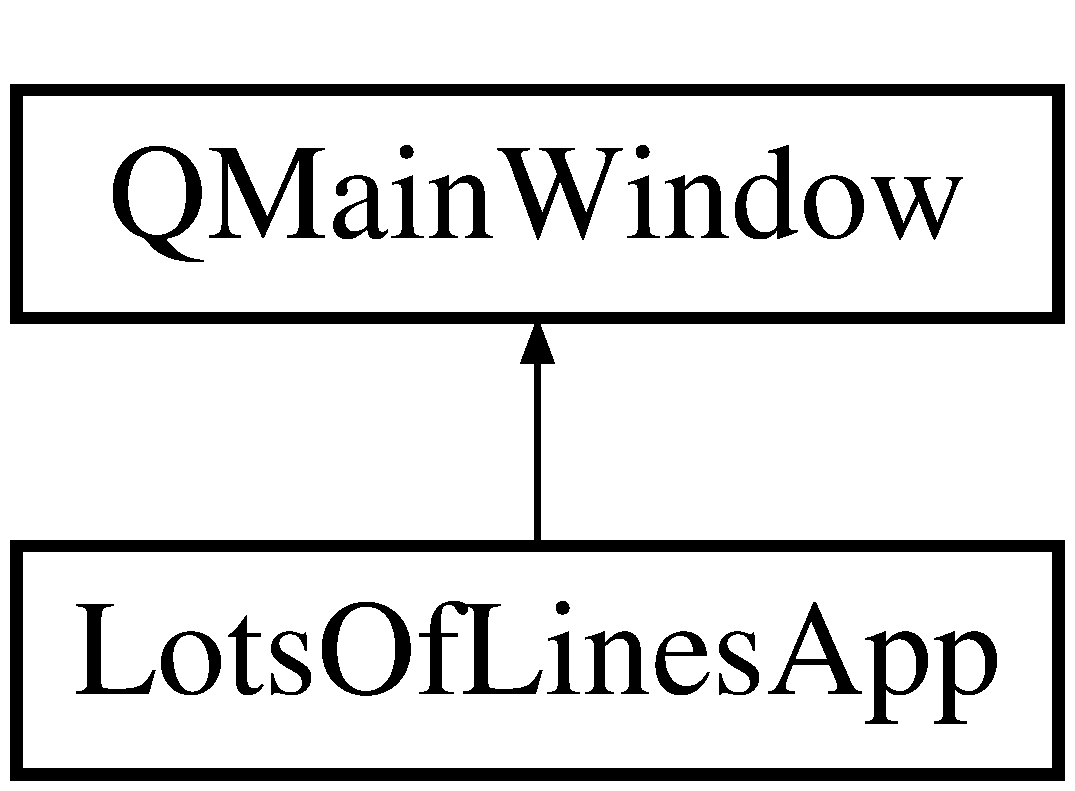
\includegraphics[height=2.000000cm]{class_lots_of_lines_app}
\end{center}
\end{figure}
\subsection*{Public Slots}
\begin{DoxyCompactItemize}
\item 
void {\bfseries add\+New\+Dataset} (std\+::shared\+\_\+ptr$<$ \hyperlink{class_lots_of_lines_1_1_data_set}{Lots\+Of\+Lines\+::\+Data\+Set} $>$)\hypertarget{class_lots_of_lines_app_af33c81460bf4947644959afedfa1574b}{}\label{class_lots_of_lines_app_af33c81460bf4947644959afedfa1574b}

\item 
void {\bfseries on\+Load\+File} ()\hypertarget{class_lots_of_lines_app_a0701fd75172ff4a0cd92bd2faba9eb41}{}\label{class_lots_of_lines_app_a0701fd75172ff4a0cd92bd2faba9eb41}

\item 
void {\bfseries on\+Open\+Preferences} ()\hypertarget{class_lots_of_lines_app_aaa0caf1c43436c86db33a5ad9babd864}{}\label{class_lots_of_lines_app_aaa0caf1c43436c86db33a5ad9babd864}

\item 
void {\bfseries on\+Visualization\+Checked} (int state)\hypertarget{class_lots_of_lines_app_abe6641f9fdc77e64232686a54bde553a}{}\label{class_lots_of_lines_app_abe6641f9fdc77e64232686a54bde553a}

\item 
void {\bfseries on\+Visualization\+Options\+Changed} (const std\+::string \&)\hypertarget{class_lots_of_lines_app_a7ec3d5c0cc49b421841f2f06c939383a}{}\label{class_lots_of_lines_app_a7ec3d5c0cc49b421841f2f06c939383a}

\end{DoxyCompactItemize}
\subsection*{Signals}
\begin{DoxyCompactItemize}
\item 
void {\bfseries request\+Dataset\+Update} (const Q\+String \&filename, const \hyperlink{struct_lots_of_lines_1_1_load_options}{Lots\+Of\+Lines\+::\+Load\+Options} \&options=Lots\+Of\+Lines\+::\+Load\+Options\+::default)\hypertarget{class_lots_of_lines_app_ac414bca34842822f3cab10f15ab8a526}{}\label{class_lots_of_lines_app_ac414bca34842822f3cab10f15ab8a526}

\end{DoxyCompactItemize}
\subsection*{Public Member Functions}
\begin{DoxyCompactItemize}
\item 
{\bfseries Lots\+Of\+Lines\+App} (const Q\+String \&open\+File, bool parallel, bool collocated\+Paired, bool radial\+Paired, bool shifted\+Paired, Q\+Widget $\ast$parent=0)\hypertarget{class_lots_of_lines_app_a4950a3d973bbcd79151485389a968546}{}\label{class_lots_of_lines_app_a4950a3d973bbcd79151485389a968546}

\item 
void \hyperlink{class_lots_of_lines_app_a1970960805f1670227d0c10bf74c8390}{load\+File} (const Q\+String \&filename, const \hyperlink{struct_lots_of_lines_1_1_load_options}{Lots\+Of\+Lines\+::\+Load\+Options} \&options=Lots\+Of\+Lines\+::\+Load\+Options\+::default)\hypertarget{class_lots_of_lines_app_a1970960805f1670227d0c10bf74c8390}{}\label{class_lots_of_lines_app_a1970960805f1670227d0c10bf74c8390}

\begin{DoxyCompactList}\small\item\em Load a data set to be displayed. \end{DoxyCompactList}\end{DoxyCompactItemize}
\subsection*{Protected Member Functions}
\begin{DoxyCompactItemize}
\item 
void \hyperlink{class_lots_of_lines_app_ad855e077f621708e535bec7122e62b17}{reload\+Data\+Table} ()\hypertarget{class_lots_of_lines_app_ad855e077f621708e535bec7122e62b17}{}\label{class_lots_of_lines_app_ad855e077f621708e535bec7122e62b17}

\begin{DoxyCompactList}\small\item\em Reloads the tabs and table models for the data table view. \end{DoxyCompactList}\item 
void \hyperlink{class_lots_of_lines_app_ad918b993305f06ac7dded3b6501e2957}{reorder\+Split\+Screens} ()\hypertarget{class_lots_of_lines_app_ad918b993305f06ac7dded3b6501e2957}{}\label{class_lots_of_lines_app_ad918b993305f06ac7dded3b6501e2957}

\begin{DoxyCompactList}\small\item\em Reorder the positions of each screen in the splitscreen layout. This must be called whenever the splitscreen widgets change, or else holes can appear in the layout. \end{DoxyCompactList}\end{DoxyCompactItemize}
\subsection*{Protected Attributes}
\begin{DoxyCompactItemize}
\item 
\hyperlink{class_ui_1_1_lots_of_lines_app_class}{Ui\+::\+Lots\+Of\+Lines\+App\+Class} {\bfseries ui}\hypertarget{class_lots_of_lines_app_a7dcf65cd508b6cf083f574a990695314}{}\label{class_lots_of_lines_app_a7dcf65cd508b6cf083f574a990695314}

\item 
std\+::shared\+\_\+ptr$<$ \hyperlink{class_lots_of_lines_1_1_data_set}{Lots\+Of\+Lines\+::\+Data\+Set} $>$ {\bfseries m\+\_\+data\+Set}\hypertarget{class_lots_of_lines_app_a58dc6cecfc94df878633f1622422b4cc}{}\label{class_lots_of_lines_app_a58dc6cecfc94df878633f1622422b4cc}

\item 
std\+::map$<$ Lots\+Of\+Lines\+::\+E\+\_\+\+V\+I\+S\+U\+A\+L\+I\+Z\+A\+T\+I\+O\+N\+\_\+\+T\+Y\+PE, \hyperlink{class_visualization_renderer_widget}{Visualization\+Renderer\+Widget} $\ast$ $>$ {\bfseries m\+\_\+renderer\+Widgets}\hypertarget{class_lots_of_lines_app_a311b80164ea07fb722dd51c4c93db430}{}\label{class_lots_of_lines_app_a311b80164ea07fb722dd51c4c93db430}

\item 
std\+::map$<$ Lots\+Of\+Lines\+::\+E\+\_\+\+V\+I\+S\+U\+A\+L\+I\+Z\+A\+T\+I\+O\+N\+\_\+\+T\+Y\+PE, \hyperlink{class_option_editor_widget}{Option\+Editor\+Widget} $\ast$ $>$ {\bfseries m\+\_\+option\+Editor\+Widgets}\hypertarget{class_lots_of_lines_app_a7df4df0a35a553e35baf49bb97e38e0a}{}\label{class_lots_of_lines_app_a7df4df0a35a553e35baf49bb97e38e0a}

\end{DoxyCompactItemize}


The documentation for this class was generated from the following files\+:\begin{DoxyCompactItemize}
\item 
D\+:/\+School/\+C\+W\+U/\+C\+S 481/\+Lots-\/of-\/\+Lines/source/Lots\+Of\+Lines\+App.\+h\item 
D\+:/\+School/\+C\+W\+U/\+C\+S 481/\+Lots-\/of-\/\+Lines/source/Lots\+Of\+Lines\+App.\+cpp\end{DoxyCompactItemize}

\hypertarget{class_ui_1_1_lots_of_lines_app_class}{}\section{Ui\+:\+:Lots\+Of\+Lines\+App\+Class Class Reference}
\label{class_ui_1_1_lots_of_lines_app_class}\index{Ui\+::\+Lots\+Of\+Lines\+App\+Class@{Ui\+::\+Lots\+Of\+Lines\+App\+Class}}
Inheritance diagram for Ui\+:\+:Lots\+Of\+Lines\+App\+Class\+:\begin{figure}[H]
\begin{center}
\leavevmode
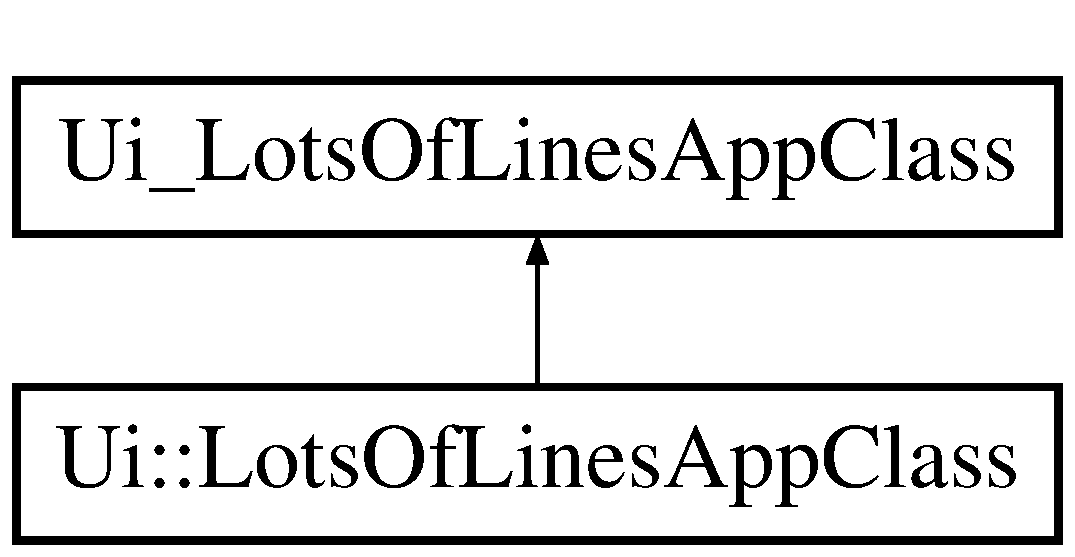
\includegraphics[height=2.000000cm]{class_ui_1_1_lots_of_lines_app_class}
\end{center}
\end{figure}
\subsection*{Additional Inherited Members}


The documentation for this class was generated from the following file\+:\begin{DoxyCompactItemize}
\item 
D\+:/\+School/\+C\+W\+U/\+C\+S 481/\+Lots-\/of-\/\+Lines/source/\+Generated\+Files/ui\+\_\+\+Lots\+Of\+Lines\+App.\+h\end{DoxyCompactItemize}

\hypertarget{struct_lots_of_lines_1_1_navigation_options}{}\section{Lots\+Of\+Lines\+:\+:Navigation\+Options Struct Reference}
\label{struct_lots_of_lines_1_1_navigation_options}\index{Lots\+Of\+Lines\+::\+Navigation\+Options@{Lots\+Of\+Lines\+::\+Navigation\+Options}}
\subsection*{Public Member Functions}
\begin{DoxyCompactItemize}
\item 
{\bfseries Navigation\+Options} (bool zX=false, bool zY=false, bool pX=false, bool pY=false, float s\+MinX=0.\+0f, float s\+Max\+X=0.\+0f)\hypertarget{struct_lots_of_lines_1_1_navigation_options_aa4123e1c1e33ce2c1dfc1a2c9d1fcf85}{}\label{struct_lots_of_lines_1_1_navigation_options_aa4123e1c1e33ce2c1dfc1a2c9d1fcf85}

\end{DoxyCompactItemize}
\subsection*{Public Attributes}
\begin{DoxyCompactItemize}
\item 
bool {\bfseries lock\+ZoomX}\hypertarget{struct_lots_of_lines_1_1_navigation_options_a81c6b99a7927e7cb34492e181b2e31bf}{}\label{struct_lots_of_lines_1_1_navigation_options_a81c6b99a7927e7cb34492e181b2e31bf}

\item 
bool {\bfseries lock\+ZoomY}\hypertarget{struct_lots_of_lines_1_1_navigation_options_ae5123c5fadd7477673249cc4d69931cd}{}\label{struct_lots_of_lines_1_1_navigation_options_ae5123c5fadd7477673249cc4d69931cd}

\item 
bool {\bfseries lock\+PanX}\hypertarget{struct_lots_of_lines_1_1_navigation_options_a7c0c9e7a00a30b7b251b87798464485e}{}\label{struct_lots_of_lines_1_1_navigation_options_a7c0c9e7a00a30b7b251b87798464485e}

\item 
bool {\bfseries lock\+PanY}\hypertarget{struct_lots_of_lines_1_1_navigation_options_a90c0cca6a2f504a5400fd04fc3b812b0}{}\label{struct_lots_of_lines_1_1_navigation_options_a90c0cca6a2f504a5400fd04fc3b812b0}

\item 
float {\bfseries min\+Scroll\+LimitX}\hypertarget{struct_lots_of_lines_1_1_navigation_options_ade7f6110db3e067a05f25c58e12758c3}{}\label{struct_lots_of_lines_1_1_navigation_options_ade7f6110db3e067a05f25c58e12758c3}

\item 
float {\bfseries max\+Scroll\+LimitX}\hypertarget{struct_lots_of_lines_1_1_navigation_options_ae357f841cbbae961c81e73c29dc4af46}{}\label{struct_lots_of_lines_1_1_navigation_options_ae357f841cbbae961c81e73c29dc4af46}

\item 
bool {\bfseries limit\+Scroll}\hypertarget{struct_lots_of_lines_1_1_navigation_options_a44171e4497aa78ae405705ae49505e04}{}\label{struct_lots_of_lines_1_1_navigation_options_a44171e4497aa78ae405705ae49505e04}

\end{DoxyCompactItemize}


The documentation for this struct was generated from the following file\+:\begin{DoxyCompactItemize}
\item 
D\+:/\+School/\+C\+W\+U/\+C\+S 481/\+Lots-\/of-\/\+Lines/source/\+Rendering\+System/I\+Visualization\+Method.\+hpp\end{DoxyCompactItemize}

\hypertarget{class_lots_of_lines_1_1_open_g_l_renderer}{}\section{Lots\+Of\+Lines\+:\+:Open\+G\+L\+Renderer Class Reference}
\label{class_lots_of_lines_1_1_open_g_l_renderer}\index{Lots\+Of\+Lines\+::\+Open\+G\+L\+Renderer@{Lots\+Of\+Lines\+::\+Open\+G\+L\+Renderer}}


Renderer implementation for drawing visualizations using Open\+GL.  




{\ttfamily \#include $<$Open\+G\+L\+Renderer.\+hpp$>$}

Inheritance diagram for Lots\+Of\+Lines\+:\+:Open\+G\+L\+Renderer\+:\begin{figure}[H]
\begin{center}
\leavevmode
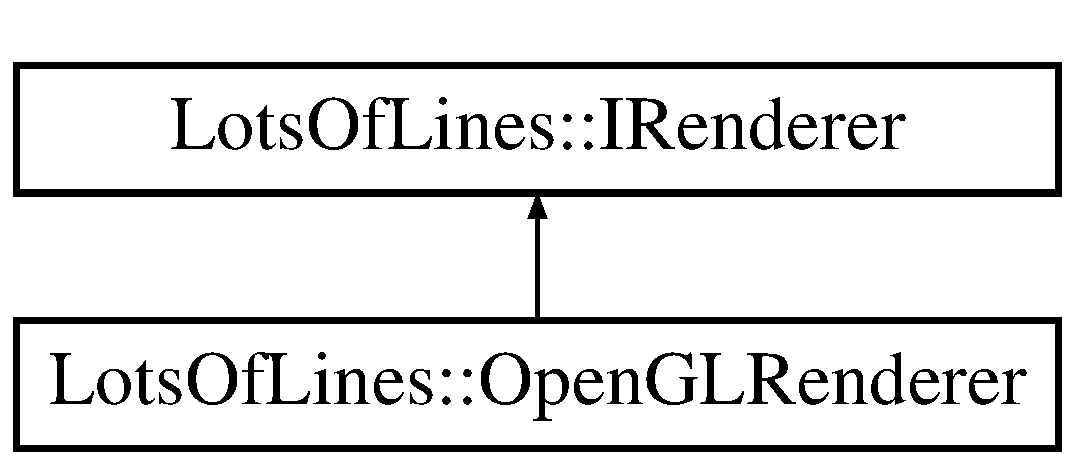
\includegraphics[height=2.000000cm]{class_lots_of_lines_1_1_open_g_l_renderer}
\end{center}
\end{figure}
\subsection*{Public Member Functions}
\begin{DoxyCompactItemize}
\item 
bool \hyperlink{class_lots_of_lines_1_1_open_g_l_renderer_a7f1cf064978a3e5f6869e54022c1d82e}{init} ()\hypertarget{class_lots_of_lines_1_1_open_g_l_renderer_a7f1cf064978a3e5f6869e54022c1d82e}{}\label{class_lots_of_lines_1_1_open_g_l_renderer_a7f1cf064978a3e5f6869e54022c1d82e}

\begin{DoxyCompactList}\small\item\em Initialize the rendering driver by setting up default shaders and rendering states. \end{DoxyCompactList}\item 
void \hyperlink{class_lots_of_lines_1_1_open_g_l_renderer_aff896e674c56136200222bce15ff8f26}{clear\+Screen} (float r, float g, float b)\hypertarget{class_lots_of_lines_1_1_open_g_l_renderer_aff896e674c56136200222bce15ff8f26}{}\label{class_lots_of_lines_1_1_open_g_l_renderer_aff896e674c56136200222bce15ff8f26}

\begin{DoxyCompactList}\small\item\em Clears the screen before re-\/rendering. \end{DoxyCompactList}\item 
void \hyperlink{class_lots_of_lines_1_1_open_g_l_renderer_a9c20e52e8c7f80d4fec614a25d507026}{begin\+Draw} ()\hypertarget{class_lots_of_lines_1_1_open_g_l_renderer_a9c20e52e8c7f80d4fec614a25d507026}{}\label{class_lots_of_lines_1_1_open_g_l_renderer_a9c20e52e8c7f80d4fec614a25d507026}

\begin{DoxyCompactList}\small\item\em Sets up rendering states to begin a frame. \end{DoxyCompactList}\item 
void \hyperlink{class_lots_of_lines_1_1_open_g_l_renderer_a57a1941507761fb0a3e12ca2a68b0066}{end\+Draw} ()\hypertarget{class_lots_of_lines_1_1_open_g_l_renderer_a57a1941507761fb0a3e12ca2a68b0066}{}\label{class_lots_of_lines_1_1_open_g_l_renderer_a57a1941507761fb0a3e12ca2a68b0066}

\begin{DoxyCompactList}\small\item\em Flips buffers to screen. \end{DoxyCompactList}\item 
void \hyperlink{class_lots_of_lines_1_1_open_g_l_renderer_aff310a706302b5961d6452451bcc9691}{set\+Class\+Colors} (float $\ast$colors)\hypertarget{class_lots_of_lines_1_1_open_g_l_renderer_aff310a706302b5961d6452451bcc9691}{}\label{class_lots_of_lines_1_1_open_g_l_renderer_aff310a706302b5961d6452451bcc9691}

\begin{DoxyCompactList}\small\item\em Set the 10x3 array of floats for colors to use when rendering the data class. \end{DoxyCompactList}\item 
void \hyperlink{class_lots_of_lines_1_1_open_g_l_renderer_ae0fc80e7572adfa6c830fbe58f1c1f5e}{set\+Viewport} (unsigned int x, unsigned int y, unsigned int width, unsigned int height)\hypertarget{class_lots_of_lines_1_1_open_g_l_renderer_ae0fc80e7572adfa6c830fbe58f1c1f5e}{}\label{class_lots_of_lines_1_1_open_g_l_renderer_ae0fc80e7572adfa6c830fbe58f1c1f5e}

\begin{DoxyCompactList}\small\item\em Set the viewport. \end{DoxyCompactList}\item 
void \hyperlink{class_lots_of_lines_1_1_open_g_l_renderer_afb420692fd26c88fafe39c85f29e030f}{set\+Model\+View\+Projection} (const glm\+::mat4x4 \&mvp)\hypertarget{class_lots_of_lines_1_1_open_g_l_renderer_afb420692fd26c88fafe39c85f29e030f}{}\label{class_lots_of_lines_1_1_open_g_l_renderer_afb420692fd26c88fafe39c85f29e030f}

\begin{DoxyCompactList}\small\item\em Set model$\ast$view$\ast$projection matrix. \end{DoxyCompactList}\item 
const glm\+::mat4x4 \& \hyperlink{class_lots_of_lines_1_1_open_g_l_renderer_a003e562c0f86b870e4fcc1f5ed0cabf0}{get\+Model\+View\+Projection} () const 
\item 
\hyperlink{class_lots_of_lines_1_1_i_shader}{I\+Shader} $\ast$ \hyperlink{class_lots_of_lines_1_1_open_g_l_renderer_afefdab5ffbe8ad3af4736ae4432f9f65}{create\+Shader} ()\hypertarget{class_lots_of_lines_1_1_open_g_l_renderer_afefdab5ffbe8ad3af4736ae4432f9f65}{}\label{class_lots_of_lines_1_1_open_g_l_renderer_afefdab5ffbe8ad3af4736ae4432f9f65}

\begin{DoxyCompactList}\small\item\em Create a new shader object. \end{DoxyCompactList}\item 
void \hyperlink{class_lots_of_lines_1_1_open_g_l_renderer_a1d11632acd909487114454857454e0c2}{set\+Shader} (\hyperlink{class_lots_of_lines_1_1_i_shader}{I\+Shader} $\ast$shader)\hypertarget{class_lots_of_lines_1_1_open_g_l_renderer_a1d11632acd909487114454857454e0c2}{}\label{class_lots_of_lines_1_1_open_g_l_renderer_a1d11632acd909487114454857454e0c2}

\begin{DoxyCompactList}\small\item\em Set the shader program to draw with. \end{DoxyCompactList}\item 
void \hyperlink{class_lots_of_lines_1_1_open_g_l_renderer_a64ec268afbae1693799dd34c3a4a399b}{draw\+V\+BO} (std\+::shared\+\_\+ptr$<$ \hyperlink{class_lots_of_lines_1_1_i_vertex_buffer_object}{I\+Vertex\+Buffer\+Object} $>$ vbo, bool lines)
\begin{DoxyCompactList}\small\item\em Draw a V\+BO to the screen. \end{DoxyCompactList}\item 
std\+::shared\+\_\+ptr$<$ \hyperlink{class_lots_of_lines_1_1_i_vertex_buffer_object}{I\+Vertex\+Buffer\+Object} $>$ \hyperlink{class_lots_of_lines_1_1_open_g_l_renderer_abf57938c51b34029efeac5c18f340213}{create\+V\+BO} (const std\+::vector$<$ \hyperlink{struct_lots_of_lines_1_1_vertex}{Vertex} $>$ \&vertices, const std\+::vector$<$ unsigned int $>$ \&indices)\hypertarget{class_lots_of_lines_1_1_open_g_l_renderer_abf57938c51b34029efeac5c18f340213}{}\label{class_lots_of_lines_1_1_open_g_l_renderer_abf57938c51b34029efeac5c18f340213}

\begin{DoxyCompactList}\small\item\em Construct a V\+BO from a list of vertices and indices. \end{DoxyCompactList}\end{DoxyCompactItemize}
\subsection*{Additional Inherited Members}


\subsection{Detailed Description}
Renderer implementation for drawing visualizations using Open\+GL. 

\subsection{Member Function Documentation}
\index{Lots\+Of\+Lines\+::\+Open\+G\+L\+Renderer@{Lots\+Of\+Lines\+::\+Open\+G\+L\+Renderer}!draw\+V\+BO@{draw\+V\+BO}}
\index{draw\+V\+BO@{draw\+V\+BO}!Lots\+Of\+Lines\+::\+Open\+G\+L\+Renderer@{Lots\+Of\+Lines\+::\+Open\+G\+L\+Renderer}}
\subsubsection[{\texorpdfstring{draw\+V\+B\+O(std\+::shared\+\_\+ptr$<$ I\+Vertex\+Buffer\+Object $>$ vbo, bool lines)}{drawVBO(std::shared_ptr< IVertexBufferObject > vbo, bool lines)}}]{\setlength{\rightskip}{0pt plus 5cm}void Open\+G\+L\+Renderer\+::draw\+V\+BO (
\begin{DoxyParamCaption}
\item[{std\+::shared\+\_\+ptr$<$ {\bf I\+Vertex\+Buffer\+Object} $>$}]{vbo, }
\item[{bool}]{lines}
\end{DoxyParamCaption}
)\hspace{0.3cm}{\ttfamily [virtual]}}\hypertarget{class_lots_of_lines_1_1_open_g_l_renderer_a64ec268afbae1693799dd34c3a4a399b}{}\label{class_lots_of_lines_1_1_open_g_l_renderer_a64ec268afbae1693799dd34c3a4a399b}


Draw a V\+BO to the screen. 


\begin{DoxyParams}{Parameters}
{\em lines} & Whether to draw as lines or points. \\
\hline
\end{DoxyParams}


Implements \hyperlink{class_lots_of_lines_1_1_i_renderer_a9d24612fea435f65dcf7d013e6693b2a}{Lots\+Of\+Lines\+::\+I\+Renderer}.

\index{Lots\+Of\+Lines\+::\+Open\+G\+L\+Renderer@{Lots\+Of\+Lines\+::\+Open\+G\+L\+Renderer}!get\+Model\+View\+Projection@{get\+Model\+View\+Projection}}
\index{get\+Model\+View\+Projection@{get\+Model\+View\+Projection}!Lots\+Of\+Lines\+::\+Open\+G\+L\+Renderer@{Lots\+Of\+Lines\+::\+Open\+G\+L\+Renderer}}
\subsubsection[{\texorpdfstring{get\+Model\+View\+Projection() const }{getModelViewProjection() const }}]{\setlength{\rightskip}{0pt plus 5cm}const glm\+::mat4x4 \& Open\+G\+L\+Renderer\+::get\+Model\+View\+Projection (
\begin{DoxyParamCaption}
{}
\end{DoxyParamCaption}
) const\hspace{0.3cm}{\ttfamily [virtual]}}\hypertarget{class_lots_of_lines_1_1_open_g_l_renderer_a003e562c0f86b870e4fcc1f5ed0cabf0}{}\label{class_lots_of_lines_1_1_open_g_l_renderer_a003e562c0f86b870e4fcc1f5ed0cabf0}
\begin{DoxyReturn}{Returns}
The currently set model$\ast$view$\ast$projection matrix. 
\end{DoxyReturn}


Implements \hyperlink{class_lots_of_lines_1_1_i_renderer_ac2c690247d805c68839ec7a831133665}{Lots\+Of\+Lines\+::\+I\+Renderer}.



The documentation for this class was generated from the following files\+:\begin{DoxyCompactItemize}
\item 
D\+:/\+School/\+C\+W\+U/\+C\+S 481/\+Lots-\/of-\/\+Lines/source/\+Rendering\+System/Open\+G\+L\+Renderer.\+hpp\item 
D\+:/\+School/\+C\+W\+U/\+C\+S 481/\+Lots-\/of-\/\+Lines/source/\+Rendering\+System/Open\+G\+L\+Renderer.\+cpp\end{DoxyCompactItemize}

\hypertarget{class_lots_of_lines_1_1_open_g_l_shader}{}\section{Lots\+Of\+Lines\+:\+:Open\+G\+L\+Shader Class Reference}
\label{class_lots_of_lines_1_1_open_g_l_shader}\index{Lots\+Of\+Lines\+::\+Open\+G\+L\+Shader@{Lots\+Of\+Lines\+::\+Open\+G\+L\+Shader}}
Inheritance diagram for Lots\+Of\+Lines\+:\+:Open\+G\+L\+Shader\+:\begin{figure}[H]
\begin{center}
\leavevmode
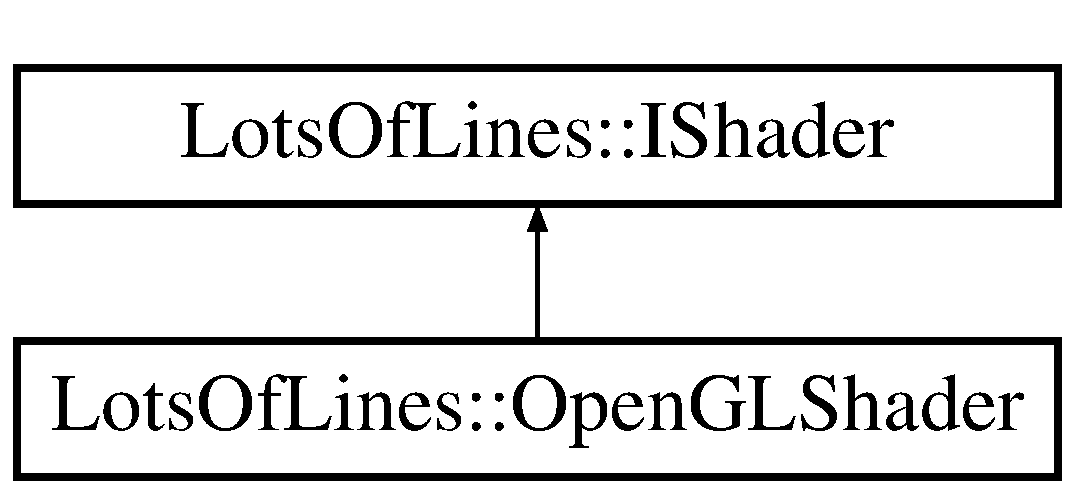
\includegraphics[height=2.000000cm]{class_lots_of_lines_1_1_open_g_l_shader}
\end{center}
\end{figure}
\subsection*{Public Member Functions}
\begin{DoxyCompactItemize}
\item 
bool \hyperlink{class_lots_of_lines_1_1_open_g_l_shader_a0993e2f4c498d275c2d4cab3775c16ce}{compile} (const char $\ast$vertex\+Shader\+Src, const char $\ast$fragment\+Shader\+Src)\hypertarget{class_lots_of_lines_1_1_open_g_l_shader_a0993e2f4c498d275c2d4cab3775c16ce}{}\label{class_lots_of_lines_1_1_open_g_l_shader_a0993e2f4c498d275c2d4cab3775c16ce}

\begin{DoxyCompactList}\small\item\em Compile a shader program from source code. \end{DoxyCompactList}\item 
unsigned int \hyperlink{class_lots_of_lines_1_1_open_g_l_shader_aba045256064bef643f0826da88fa7450}{get\+Program} () const 
\end{DoxyCompactItemize}


\subsection{Member Function Documentation}
\index{Lots\+Of\+Lines\+::\+Open\+G\+L\+Shader@{Lots\+Of\+Lines\+::\+Open\+G\+L\+Shader}!get\+Program@{get\+Program}}
\index{get\+Program@{get\+Program}!Lots\+Of\+Lines\+::\+Open\+G\+L\+Shader@{Lots\+Of\+Lines\+::\+Open\+G\+L\+Shader}}
\subsubsection[{\texorpdfstring{get\+Program() const }{getProgram() const }}]{\setlength{\rightskip}{0pt plus 5cm}unsigned int Open\+G\+L\+Shader\+::get\+Program (
\begin{DoxyParamCaption}
{}
\end{DoxyParamCaption}
) const}\hypertarget{class_lots_of_lines_1_1_open_g_l_shader_aba045256064bef643f0826da88fa7450}{}\label{class_lots_of_lines_1_1_open_g_l_shader_aba045256064bef643f0826da88fa7450}
\begin{DoxyReturn}{Returns}
The compiled G\+L\+SL program. 
\end{DoxyReturn}


The documentation for this class was generated from the following files\+:\begin{DoxyCompactItemize}
\item 
D\+:/\+School/\+C\+W\+U/\+C\+S 481/\+Lots-\/of-\/\+Lines/source/\+Rendering\+System/Open\+G\+L\+Shader.\+hpp\item 
D\+:/\+School/\+C\+W\+U/\+C\+S 481/\+Lots-\/of-\/\+Lines/source/\+Rendering\+System/Open\+G\+L\+Shader.\+cpp\end{DoxyCompactItemize}

\hypertarget{class_lots_of_lines_1_1_open_g_l_vertex_buffer_object}{}\section{Lots\+Of\+Lines\+:\+:Open\+G\+L\+Vertex\+Buffer\+Object Class Reference}
\label{class_lots_of_lines_1_1_open_g_l_vertex_buffer_object}\index{Lots\+Of\+Lines\+::\+Open\+G\+L\+Vertex\+Buffer\+Object@{Lots\+Of\+Lines\+::\+Open\+G\+L\+Vertex\+Buffer\+Object}}
Inheritance diagram for Lots\+Of\+Lines\+:\+:Open\+G\+L\+Vertex\+Buffer\+Object\+:\begin{figure}[H]
\begin{center}
\leavevmode
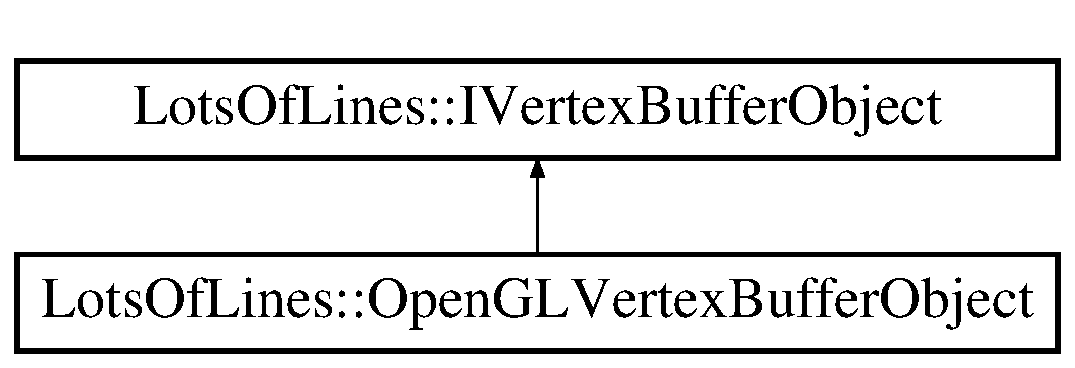
\includegraphics[height=2.000000cm]{class_lots_of_lines_1_1_open_g_l_vertex_buffer_object}
\end{center}
\end{figure}
\subsection*{Public Member Functions}
\begin{DoxyCompactItemize}
\item 
bool {\bfseries init} (const std\+::vector$<$ \hyperlink{struct_lots_of_lines_1_1_vertex}{Vertex} $>$ \&vertices, const std\+::vector$<$ unsigned int $>$ \&indices)\hypertarget{class_lots_of_lines_1_1_open_g_l_vertex_buffer_object_a5c7e13ab9c0d5baba3aba0bf1bb2bb22}{}\label{class_lots_of_lines_1_1_open_g_l_vertex_buffer_object_a5c7e13ab9c0d5baba3aba0bf1bb2bb22}

\item 
\hyperlink{struct_lots_of_lines_1_1_vertex}{Vertex} $\ast$ \hyperlink{class_lots_of_lines_1_1_open_g_l_vertex_buffer_object_a842ae500f862c5fb011ce1fa93478236}{map\+Vertices} (bool read\+Only=false)
\begin{DoxyCompactList}\small\item\em Map the vertex buffer for access. \end{DoxyCompactList}\item 
void \hyperlink{class_lots_of_lines_1_1_open_g_l_vertex_buffer_object_ad3e09ea6ff43545352e9df6da5072beb}{unmap\+Vertices} ()\hypertarget{class_lots_of_lines_1_1_open_g_l_vertex_buffer_object_ad3e09ea6ff43545352e9df6da5072beb}{}\label{class_lots_of_lines_1_1_open_g_l_vertex_buffer_object_ad3e09ea6ff43545352e9df6da5072beb}

\begin{DoxyCompactList}\small\item\em Unmap (unlock) the vertex buffer after accessing it. \end{DoxyCompactList}\item 
unsigned int $\ast$ \hyperlink{class_lots_of_lines_1_1_open_g_l_vertex_buffer_object_a59c71c761341ca1732b5816bdfe6d239}{map\+Indices} ()
\begin{DoxyCompactList}\small\item\em Map the index buffer for access. \end{DoxyCompactList}\item 
void \hyperlink{class_lots_of_lines_1_1_open_g_l_vertex_buffer_object_ad0c16f10859218f09a42ffbd4dd747b0}{unmap\+Indices} ()\hypertarget{class_lots_of_lines_1_1_open_g_l_vertex_buffer_object_ad0c16f10859218f09a42ffbd4dd747b0}{}\label{class_lots_of_lines_1_1_open_g_l_vertex_buffer_object_ad0c16f10859218f09a42ffbd4dd747b0}

\begin{DoxyCompactList}\small\item\em Unmap (unlock) the index buffer after accessing it. \end{DoxyCompactList}\item 
unsigned int {\bfseries vertex\+Count} () const \hypertarget{class_lots_of_lines_1_1_open_g_l_vertex_buffer_object_af82a0102fd076c0707c6e14ef1b8eb04}{}\label{class_lots_of_lines_1_1_open_g_l_vertex_buffer_object_af82a0102fd076c0707c6e14ef1b8eb04}

\item 
unsigned int {\bfseries index\+Count} () const \hypertarget{class_lots_of_lines_1_1_open_g_l_vertex_buffer_object_a433ac651d6ba21320d40ca2dd6c3dbf6}{}\label{class_lots_of_lines_1_1_open_g_l_vertex_buffer_object_a433ac651d6ba21320d40ca2dd6c3dbf6}

\item 
void {\bfseries draw} (bool lines=true)\hypertarget{class_lots_of_lines_1_1_open_g_l_vertex_buffer_object_acb47d279820505f869807a4df6b18ace}{}\label{class_lots_of_lines_1_1_open_g_l_vertex_buffer_object_acb47d279820505f869807a4df6b18ace}

\end{DoxyCompactItemize}


\subsection{Member Function Documentation}
\index{Lots\+Of\+Lines\+::\+Open\+G\+L\+Vertex\+Buffer\+Object@{Lots\+Of\+Lines\+::\+Open\+G\+L\+Vertex\+Buffer\+Object}!map\+Indices@{map\+Indices}}
\index{map\+Indices@{map\+Indices}!Lots\+Of\+Lines\+::\+Open\+G\+L\+Vertex\+Buffer\+Object@{Lots\+Of\+Lines\+::\+Open\+G\+L\+Vertex\+Buffer\+Object}}
\subsubsection[{\texorpdfstring{map\+Indices()}{mapIndices()}}]{\setlength{\rightskip}{0pt plus 5cm}unsigned int $\ast$ Open\+G\+L\+Vertex\+Buffer\+Object\+::map\+Indices (
\begin{DoxyParamCaption}
{}
\end{DoxyParamCaption}
)\hspace{0.3cm}{\ttfamily [virtual]}}\hypertarget{class_lots_of_lines_1_1_open_g_l_vertex_buffer_object_a59c71c761341ca1732b5816bdfe6d239}{}\label{class_lots_of_lines_1_1_open_g_l_vertex_buffer_object_a59c71c761341ca1732b5816bdfe6d239}


Map the index buffer for access. 

\begin{DoxyReturn}{Returns}
A pointer to the index buffer\textquotesingle{}s data, or N\+U\+LL if the buffer couldn\textquotesingle{}t be mapped. 
\end{DoxyReturn}


Implements \hyperlink{class_lots_of_lines_1_1_i_vertex_buffer_object_a8820943ddcb998bccb03a9769611218b}{Lots\+Of\+Lines\+::\+I\+Vertex\+Buffer\+Object}.

\index{Lots\+Of\+Lines\+::\+Open\+G\+L\+Vertex\+Buffer\+Object@{Lots\+Of\+Lines\+::\+Open\+G\+L\+Vertex\+Buffer\+Object}!map\+Vertices@{map\+Vertices}}
\index{map\+Vertices@{map\+Vertices}!Lots\+Of\+Lines\+::\+Open\+G\+L\+Vertex\+Buffer\+Object@{Lots\+Of\+Lines\+::\+Open\+G\+L\+Vertex\+Buffer\+Object}}
\subsubsection[{\texorpdfstring{map\+Vertices(bool read\+Only=false)}{mapVertices(bool readOnly=false)}}]{\setlength{\rightskip}{0pt plus 5cm}{\bf Vertex} $\ast$ Open\+G\+L\+Vertex\+Buffer\+Object\+::map\+Vertices (
\begin{DoxyParamCaption}
\item[{bool}]{read\+Only = {\ttfamily false}}
\end{DoxyParamCaption}
)\hspace{0.3cm}{\ttfamily [virtual]}}\hypertarget{class_lots_of_lines_1_1_open_g_l_vertex_buffer_object_a842ae500f862c5fb011ce1fa93478236}{}\label{class_lots_of_lines_1_1_open_g_l_vertex_buffer_object_a842ae500f862c5fb011ce1fa93478236}


Map the vertex buffer for access. 

\begin{DoxyReturn}{Returns}
A pointer to the vertex buffer\textquotesingle{}s data, or N\+U\+LL if the buffer couldn\textquotesingle{}t be mapped. 
\end{DoxyReturn}


Implements \hyperlink{class_lots_of_lines_1_1_i_vertex_buffer_object_ae367bf3f773738ffb1bf6957dba1cc13}{Lots\+Of\+Lines\+::\+I\+Vertex\+Buffer\+Object}.



The documentation for this class was generated from the following files\+:\begin{DoxyCompactItemize}
\item 
D\+:/\+School/\+C\+W\+U/\+C\+S 481/\+Lots-\/of-\/\+Lines/source/\+Rendering\+System/Open\+G\+L\+Vertex\+Buffer\+Object.\+hpp\item 
D\+:/\+School/\+C\+W\+U/\+C\+S 481/\+Lots-\/of-\/\+Lines/source/\+Rendering\+System/Open\+G\+L\+Vertex\+Buffer\+Object.\+cpp\end{DoxyCompactItemize}

\hypertarget{class_option_editor_widget}{}\section{Option\+Editor\+Widget Class Reference}
\label{class_option_editor_widget}\index{Option\+Editor\+Widget@{Option\+Editor\+Widget}}


Widget for modifying generic options object.  




{\ttfamily \#include $<$Option\+Editor\+Widget.\+h$>$}

Inheritance diagram for Option\+Editor\+Widget\+:\begin{figure}[H]
\begin{center}
\leavevmode
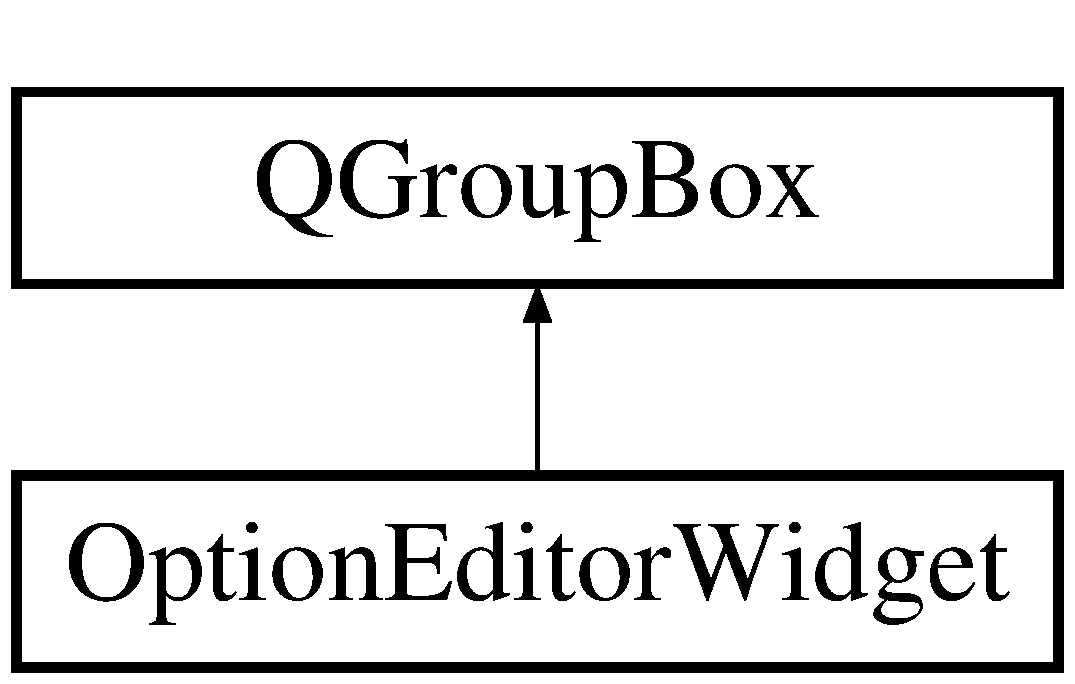
\includegraphics[height=2.000000cm]{class_option_editor_widget}
\end{center}
\end{figure}
\subsection*{Public Slots}
\begin{DoxyCompactItemize}
\item 
void {\bfseries on\+Checkbox\+Changed} (int state)\hypertarget{class_option_editor_widget_af091fec5c4f6c40173be3656fd041c12}{}\label{class_option_editor_widget_af091fec5c4f6c40173be3656fd041c12}

\item 
void {\bfseries on\+Text\+Edited} (const Q\+String \&text)\hypertarget{class_option_editor_widget_ac7b1308fcee65a92a47c7776582dc5f6}{}\label{class_option_editor_widget_ac7b1308fcee65a92a47c7776582dc5f6}

\item 
void {\bfseries on\+Int\+Changed} (int n)\hypertarget{class_option_editor_widget_a6c52fc4d311d806b5a66fc398db21eba}{}\label{class_option_editor_widget_a6c52fc4d311d806b5a66fc398db21eba}

\item 
void {\bfseries on\+Double\+Changed} (double n)\hypertarget{class_option_editor_widget_a00985b7680ba7d8f01ab555e7301093e}{}\label{class_option_editor_widget_a00985b7680ba7d8f01ab555e7301093e}

\end{DoxyCompactItemize}
\subsection*{Signals}
\begin{DoxyCompactItemize}
\item 
void \hyperlink{class_option_editor_widget_a5d20206fb9e29ea1e342d423d1a10eed}{option\+Changed} (const std\+::string \&name)\hypertarget{class_option_editor_widget_a5d20206fb9e29ea1e342d423d1a10eed}{}\label{class_option_editor_widget_a5d20206fb9e29ea1e342d423d1a10eed}

\begin{DoxyCompactList}\small\item\em Signal emitted when an option changes. \end{DoxyCompactList}\end{DoxyCompactItemize}
\subsection*{Public Member Functions}
\begin{DoxyCompactItemize}
\item 
{\bfseries Option\+Editor\+Widget} (const Q\+String \&title, \hyperlink{class_lots_of_lines_1_1_visualization_options}{Lots\+Of\+Lines\+::\+Visualization\+Options} \&options, Q\+Widget $\ast$parent=0)\hypertarget{class_option_editor_widget_ad4a9335b2399f860b13e925a7eff834d}{}\label{class_option_editor_widget_ad4a9335b2399f860b13e925a7eff834d}

\end{DoxyCompactItemize}
\subsection*{Public Attributes}
\begin{DoxyCompactItemize}
\item 
void $\ast$ {\bfseries user\+Pointer} = nullptr\hypertarget{class_option_editor_widget_ab6be94155c50503af258f0cc9da45c04}{}\label{class_option_editor_widget_ab6be94155c50503af258f0cc9da45c04}

\end{DoxyCompactItemize}


\subsection{Detailed Description}
Widget for modifying generic options object. 

The documentation for this class was generated from the following files\+:\begin{DoxyCompactItemize}
\item 
D\+:/\+School/\+C\+W\+U/\+C\+S 481/\+Lots-\/of-\/\+Lines/source/Option\+Editor\+Widget.\+h\item 
D\+:/\+School/\+C\+W\+U/\+C\+S 481/\+Lots-\/of-\/\+Lines/source/Option\+Editor\+Widget.\+cpp\end{DoxyCompactItemize}

\hypertarget{class_lots_of_lines_1_1_parallel_coordinates_visualization_method}{}\section{Lots\+Of\+Lines\+:\+:Parallel\+Coordinates\+Visualization\+Method Class Reference}
\label{class_lots_of_lines_1_1_parallel_coordinates_visualization_method}\index{Lots\+Of\+Lines\+::\+Parallel\+Coordinates\+Visualization\+Method@{Lots\+Of\+Lines\+::\+Parallel\+Coordinates\+Visualization\+Method}}
Inheritance diagram for Lots\+Of\+Lines\+:\+:Parallel\+Coordinates\+Visualization\+Method\+:\begin{figure}[H]
\begin{center}
\leavevmode
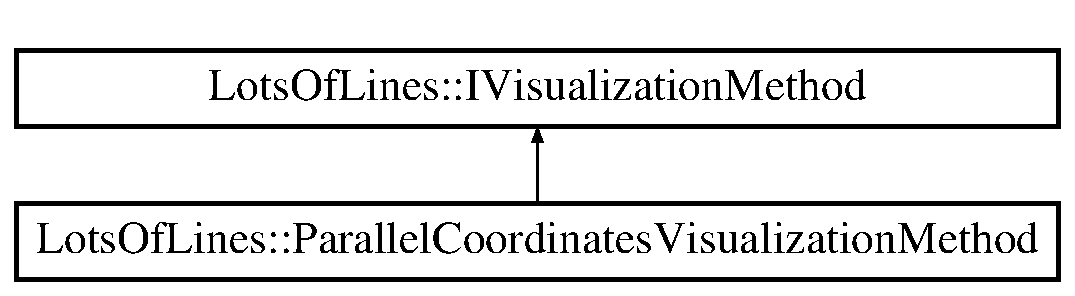
\includegraphics[height=2.000000cm]{class_lots_of_lines_1_1_parallel_coordinates_visualization_method}
\end{center}
\end{figure}
\subsection*{Public Member Functions}
\begin{DoxyCompactItemize}
\item 
void \hyperlink{class_lots_of_lines_1_1_parallel_coordinates_visualization_method_a9fc4a16e5616115ad9e8c983fefb80ab}{get\+Navigation\+Options} (\hyperlink{struct_lots_of_lines_1_1_navigation_options}{Navigation\+Options} \&options\+Out)\hypertarget{class_lots_of_lines_1_1_parallel_coordinates_visualization_method_a9fc4a16e5616115ad9e8c983fefb80ab}{}\label{class_lots_of_lines_1_1_parallel_coordinates_visualization_method_a9fc4a16e5616115ad9e8c983fefb80ab}

\begin{DoxyCompactList}\small\item\em Should return the navigation options for the rendering method (X scroll lock, etc) \end{DoxyCompactList}\item 
void \hyperlink{class_lots_of_lines_1_1_parallel_coordinates_visualization_method_a47f47082f6638364ca12c521b8520e30}{get\+Default\+Options} (\hyperlink{class_lots_of_lines_1_1_visualization_options}{Visualization\+Options} \&options)\hypertarget{class_lots_of_lines_1_1_parallel_coordinates_visualization_method_a47f47082f6638364ca12c521b8520e30}{}\label{class_lots_of_lines_1_1_parallel_coordinates_visualization_method_a47f47082f6638364ca12c521b8520e30}

\begin{DoxyCompactList}\small\item\em Should fill an empty \hyperlink{class_lots_of_lines_1_1_visualization_options}{Visualization\+Options} object with the default options to use for the visualization method. This method will be called once when the visualization method is loaded in order to generate fields for the UI system. \end{DoxyCompactList}\item 
bool \hyperlink{class_lots_of_lines_1_1_parallel_coordinates_visualization_method_a4c08598cae13367a5b77828be347ac2e}{generate\+V\+BO} (const std\+::shared\+\_\+ptr$<$ const \hyperlink{class_lots_of_lines_1_1_data_set}{Data\+Set} $>$ data\+Set, std\+::vector$<$ \hyperlink{struct_lots_of_lines_1_1_vertex}{Vertex} $>$ \&vertices\+Out, std\+::vector$<$ unsigned int $>$ \&indices\+Out, \hyperlink{class_lots_of_lines_1_1_rendering_system}{Rendering\+System} $\ast$driver, const \hyperlink{class_lots_of_lines_1_1_visualization_options}{Visualization\+Options} \&options)\hypertarget{class_lots_of_lines_1_1_parallel_coordinates_visualization_method_a4c08598cae13367a5b77828be347ac2e}{}\label{class_lots_of_lines_1_1_parallel_coordinates_visualization_method_a4c08598cae13367a5b77828be347ac2e}

\begin{DoxyCompactList}\small\item\em Generate a vertex buffer for the visualization. \end{DoxyCompactList}\item 
void \hyperlink{class_lots_of_lines_1_1_parallel_coordinates_visualization_method_a2df2c91354041c193e4055aeac7cfad2}{pre\+Draw} (\hyperlink{class_lots_of_lines_1_1_rendering_system}{Rendering\+System} $\ast$driver)\hypertarget{class_lots_of_lines_1_1_parallel_coordinates_visualization_method_a2df2c91354041c193e4055aeac7cfad2}{}\label{class_lots_of_lines_1_1_parallel_coordinates_visualization_method_a2df2c91354041c193e4055aeac7cfad2}

\begin{DoxyCompactList}\small\item\em Draw axis lines and other extra features of the visualization method. \end{DoxyCompactList}\end{DoxyCompactItemize}
\subsection*{Public Attributes}
\begin{DoxyCompactItemize}
\item 
const char $\ast$ {\bfseries F\+I\+T\+\_\+\+T\+O\+\_\+\+S\+C\+R\+E\+E\+N\+\_\+\+H\+O\+R\+I\+Z\+O\+N\+T\+AL} = \char`\"{}Fit horizontal\char`\"{}\hypertarget{class_lots_of_lines_1_1_parallel_coordinates_visualization_method_aefad54ada3adf700219394f34e862162}{}\label{class_lots_of_lines_1_1_parallel_coordinates_visualization_method_aefad54ada3adf700219394f34e862162}

\item 
const char $\ast$ {\bfseries S\+H\+I\+F\+T\+ED} = \char`\"{}Shift axes based around central line\char`\"{}\hypertarget{class_lots_of_lines_1_1_parallel_coordinates_visualization_method_a6800a60bb4e99b4f58d45affdf46a314}{}\label{class_lots_of_lines_1_1_parallel_coordinates_visualization_method_a6800a60bb4e99b4f58d45affdf46a314}

\item 
const char $\ast$ {\bfseries A\+X\+I\+S\+\_\+\+S\+P\+A\+C\+I\+NG} = \char`\"{}Axis spacing\char`\"{}\hypertarget{class_lots_of_lines_1_1_parallel_coordinates_visualization_method_abb6773006f0f62973b62093a6b1ca987}{}\label{class_lots_of_lines_1_1_parallel_coordinates_visualization_method_abb6773006f0f62973b62093a6b1ca987}

\item 
float {\bfseries m\+\_\+scroll\+Limit} = 0.\+0f\hypertarget{class_lots_of_lines_1_1_parallel_coordinates_visualization_method_a70616701546af28d381850d6761d3acf}{}\label{class_lots_of_lines_1_1_parallel_coordinates_visualization_method_a70616701546af28d381850d6761d3acf}

\end{DoxyCompactItemize}


The documentation for this class was generated from the following files\+:\begin{DoxyCompactItemize}
\item 
D\+:/\+School/\+C\+W\+U/\+C\+S 481/\+Lots-\/of-\/\+Lines/source/\+Rendering\+System/Parallel\+Coordinates\+Visualization\+Method.\+hpp\item 
D\+:/\+School/\+C\+W\+U/\+C\+S 481/\+Lots-\/of-\/\+Lines/source/\+Rendering\+System/Parallel\+Coordinates\+Visualization\+Method.\+cpp\end{DoxyCompactItemize}

\hypertarget{class_preferences_dialog}{}\section{Preferences\+Dialog Class Reference}
\label{class_preferences_dialog}\index{Preferences\+Dialog@{Preferences\+Dialog}}
Inheritance diagram for Preferences\+Dialog\+:\begin{figure}[H]
\begin{center}
\leavevmode
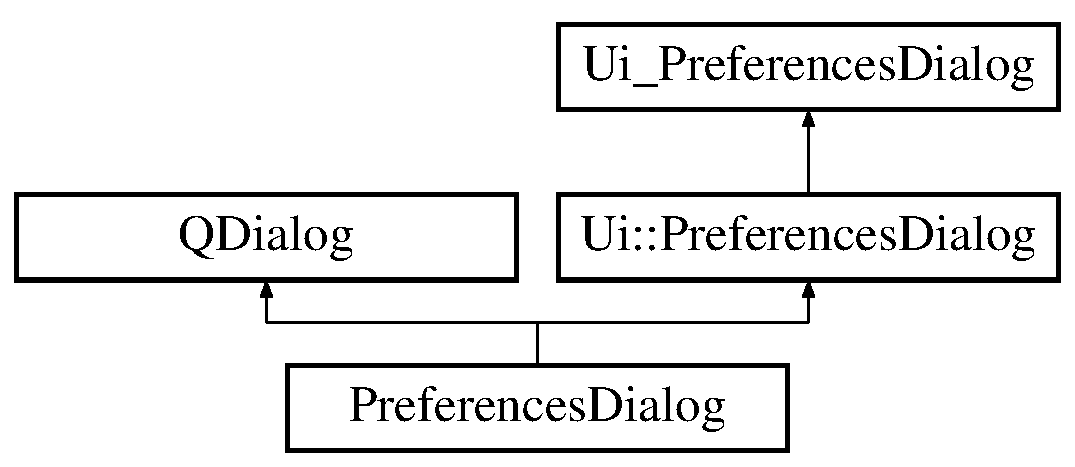
\includegraphics[height=3.000000cm]{class_preferences_dialog}
\end{center}
\end{figure}
\subsection*{Public Member Functions}
\begin{DoxyCompactItemize}
\item 
{\bfseries Preferences\+Dialog} (Q\+Widget $\ast$parent)\hypertarget{class_preferences_dialog_ab98d8a3516f8ecb7e117b87e13827180}{}\label{class_preferences_dialog_ab98d8a3516f8ecb7e117b87e13827180}

\end{DoxyCompactItemize}
\subsection*{Additional Inherited Members}


The documentation for this class was generated from the following files\+:\begin{DoxyCompactItemize}
\item 
D\+:/\+School/\+C\+W\+U/\+C\+S 481/\+Lots-\/of-\/\+Lines/source/Preferences\+Dialog.\+h\item 
D\+:/\+School/\+C\+W\+U/\+C\+S 481/\+Lots-\/of-\/\+Lines/source/Preferences\+Dialog.\+cpp\end{DoxyCompactItemize}

\hypertarget{class_ui_1_1_preferences_dialog}{}\section{Ui\+:\+:Preferences\+Dialog Class Reference}
\label{class_ui_1_1_preferences_dialog}\index{Ui\+::\+Preferences\+Dialog@{Ui\+::\+Preferences\+Dialog}}
Inheritance diagram for Ui\+:\+:Preferences\+Dialog\+:\begin{figure}[H]
\begin{center}
\leavevmode
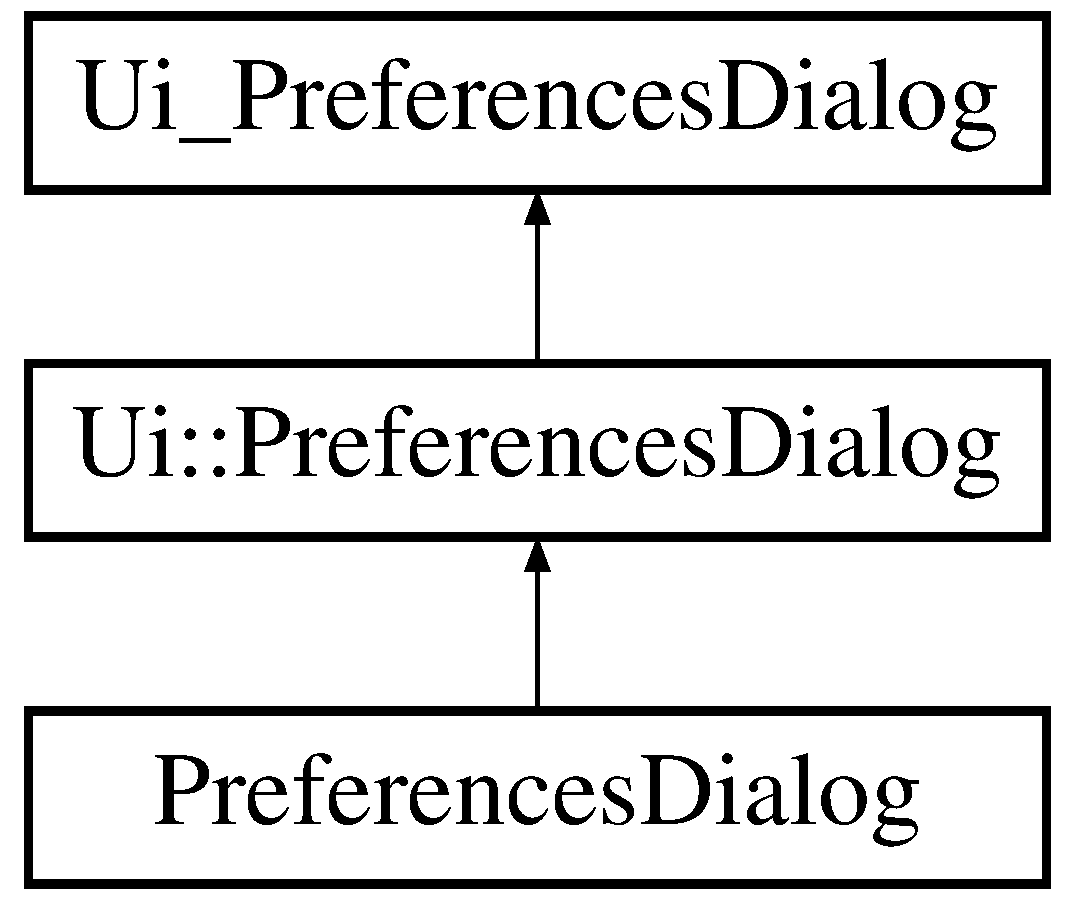
\includegraphics[height=3.000000cm]{class_ui_1_1_preferences_dialog}
\end{center}
\end{figure}
\subsection*{Additional Inherited Members}


The documentation for this class was generated from the following file\+:\begin{DoxyCompactItemize}
\item 
D\+:/\+School/\+C\+W\+U/\+C\+S 481/\+Lots-\/of-\/\+Lines/source/\+Generated\+Files/ui\+\_\+\+Preferences\+Dialog.\+h\end{DoxyCompactItemize}

\hypertarget{class_lots_of_lines_1_1_progress_message}{}\section{Lots\+Of\+Lines\+:\+:Progress\+Message Class Reference}
\label{class_lots_of_lines_1_1_progress_message}\index{Lots\+Of\+Lines\+::\+Progress\+Message@{Lots\+Of\+Lines\+::\+Progress\+Message}}
Inheritance diagram for Lots\+Of\+Lines\+:\+:Progress\+Message\+:\begin{figure}[H]
\begin{center}
\leavevmode
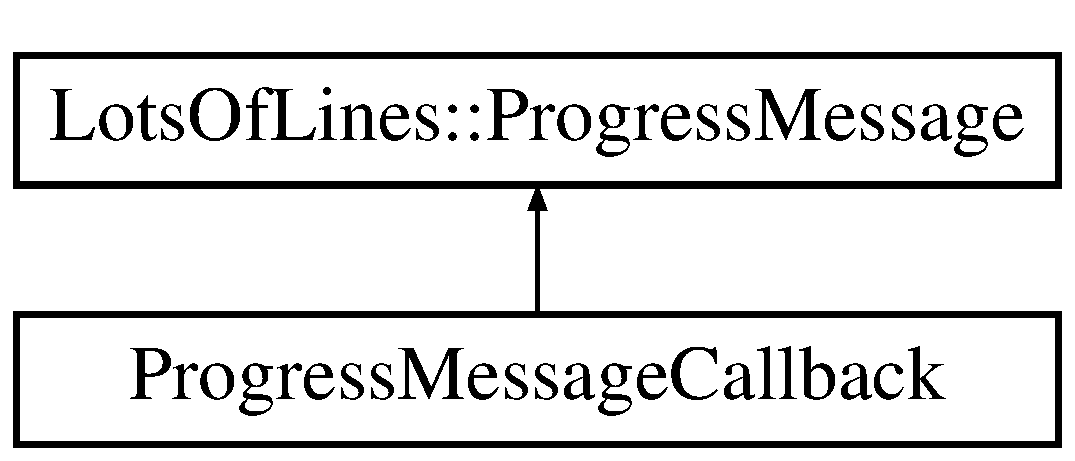
\includegraphics[height=2.000000cm]{class_lots_of_lines_1_1_progress_message}
\end{center}
\end{figure}
\subsection*{Public Member Functions}
\begin{DoxyCompactItemize}
\item 
virtual void {\bfseries progress} (int p)=0\hypertarget{class_lots_of_lines_1_1_progress_message_a216b524c5e4680dea556a68547daab5d}{}\label{class_lots_of_lines_1_1_progress_message_a216b524c5e4680dea556a68547daab5d}

\end{DoxyCompactItemize}


The documentation for this class was generated from the following file\+:\begin{DoxyCompactItemize}
\item 
D\+:/\+School/\+C\+W\+U/\+C\+S 481/\+Lots-\/of-\/\+Lines/source/\+Data\+Model/Progress\+Message.\+hpp\end{DoxyCompactItemize}

\hypertarget{class_progress_message_callback}{}\section{Progress\+Message\+Callback Class Reference}
\label{class_progress_message_callback}\index{Progress\+Message\+Callback@{Progress\+Message\+Callback}}
Inheritance diagram for Progress\+Message\+Callback\+:\begin{figure}[H]
\begin{center}
\leavevmode
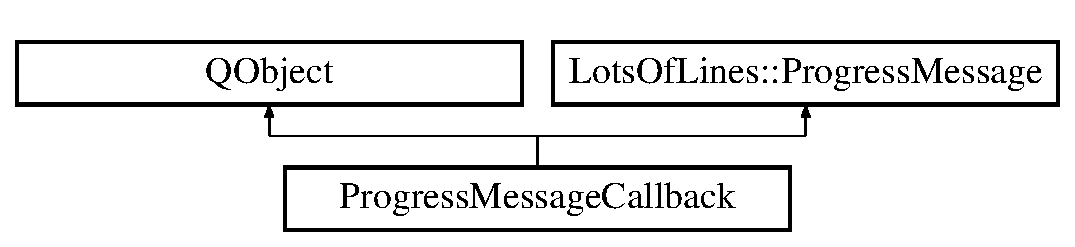
\includegraphics[height=2.000000cm]{class_progress_message_callback}
\end{center}
\end{figure}
\subsection*{Signals}
\begin{DoxyCompactItemize}
\item 
void {\bfseries progress\+Signal} (const int \&p)\hypertarget{class_progress_message_callback_a8d47a5048f6b10874a6bf4f874830b64}{}\label{class_progress_message_callback_a8d47a5048f6b10874a6bf4f874830b64}

\end{DoxyCompactItemize}
\subsection*{Public Member Functions}
\begin{DoxyCompactItemize}
\item 
{\bfseries Progress\+Message\+Callback} (Q\+Progress\+Dialog \&gui)\hypertarget{class_progress_message_callback_a212a38b4df9aef9b1dd35f5d1c961b86}{}\label{class_progress_message_callback_a212a38b4df9aef9b1dd35f5d1c961b86}

\item 
virtual void {\bfseries progress} (int p)\hypertarget{class_progress_message_callback_ad3e87c2805aa0fe02f207d40923fa928}{}\label{class_progress_message_callback_ad3e87c2805aa0fe02f207d40923fa928}

\end{DoxyCompactItemize}


The documentation for this class was generated from the following file\+:\begin{DoxyCompactItemize}
\item 
D\+:/\+School/\+C\+W\+U/\+C\+S 481/\+Lots-\/of-\/\+Lines/source/Lots\+Of\+Lines\+App.\+h\end{DoxyCompactItemize}

\hypertarget{class_lots_of_lines_1_1_radial_paired_coordinates_visualization_method}{}\section{Lots\+Of\+Lines\+:\+:Radial\+Paired\+Coordinates\+Visualization\+Method Class Reference}
\label{class_lots_of_lines_1_1_radial_paired_coordinates_visualization_method}\index{Lots\+Of\+Lines\+::\+Radial\+Paired\+Coordinates\+Visualization\+Method@{Lots\+Of\+Lines\+::\+Radial\+Paired\+Coordinates\+Visualization\+Method}}
Inheritance diagram for Lots\+Of\+Lines\+:\+:Radial\+Paired\+Coordinates\+Visualization\+Method\+:\begin{figure}[H]
\begin{center}
\leavevmode
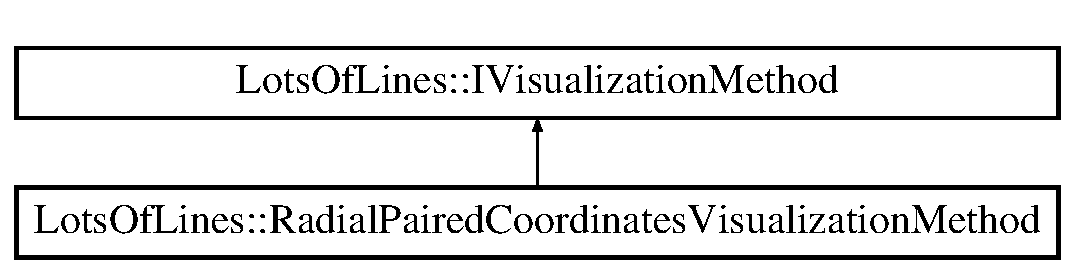
\includegraphics[height=2.000000cm]{class_lots_of_lines_1_1_radial_paired_coordinates_visualization_method}
\end{center}
\end{figure}
\subsection*{Public Member Functions}
\begin{DoxyCompactItemize}
\item 
void \hyperlink{class_lots_of_lines_1_1_radial_paired_coordinates_visualization_method_ad7462567a3662995723e0fb11b89ea69}{get\+Navigation\+Options} (\hyperlink{struct_lots_of_lines_1_1_navigation_options}{Navigation\+Options} \&options\+Out)\hypertarget{class_lots_of_lines_1_1_radial_paired_coordinates_visualization_method_ad7462567a3662995723e0fb11b89ea69}{}\label{class_lots_of_lines_1_1_radial_paired_coordinates_visualization_method_ad7462567a3662995723e0fb11b89ea69}

\begin{DoxyCompactList}\small\item\em Should return the navigation options for the rendering method (X scroll lock, etc) \end{DoxyCompactList}\item 
void \hyperlink{class_lots_of_lines_1_1_radial_paired_coordinates_visualization_method_ae1ecc6a006aed89f4716eed79257b764}{get\+Default\+Options} (\hyperlink{class_lots_of_lines_1_1_visualization_options}{Visualization\+Options} \&options)\hypertarget{class_lots_of_lines_1_1_radial_paired_coordinates_visualization_method_ae1ecc6a006aed89f4716eed79257b764}{}\label{class_lots_of_lines_1_1_radial_paired_coordinates_visualization_method_ae1ecc6a006aed89f4716eed79257b764}

\begin{DoxyCompactList}\small\item\em Should fill an empty \hyperlink{class_lots_of_lines_1_1_visualization_options}{Visualization\+Options} object with the default options to use for the visualization method. This method will be called once when the visualization method is loaded in order to generate fields for the UI system. \end{DoxyCompactList}\item 
bool \hyperlink{class_lots_of_lines_1_1_radial_paired_coordinates_visualization_method_ae47504a4cc82235dc02ffabd26fb1657}{generate\+V\+BO} (const std\+::shared\+\_\+ptr$<$ const \hyperlink{class_lots_of_lines_1_1_data_set}{Data\+Set} $>$ data\+Set, std\+::vector$<$ \hyperlink{struct_lots_of_lines_1_1_vertex}{Vertex} $>$ \&vertices\+Out, std\+::vector$<$ unsigned int $>$ \&indices\+Out, \hyperlink{class_lots_of_lines_1_1_rendering_system}{Rendering\+System} $\ast$driver, const \hyperlink{class_lots_of_lines_1_1_visualization_options}{Visualization\+Options} \&options)\hypertarget{class_lots_of_lines_1_1_radial_paired_coordinates_visualization_method_ae47504a4cc82235dc02ffabd26fb1657}{}\label{class_lots_of_lines_1_1_radial_paired_coordinates_visualization_method_ae47504a4cc82235dc02ffabd26fb1657}

\begin{DoxyCompactList}\small\item\em Generate a vertex buffer for the visualization. \end{DoxyCompactList}\end{DoxyCompactItemize}
\subsection*{Public Attributes}
\begin{DoxyCompactItemize}
\item 
const char $\ast$ {\bfseries D\+R\+A\+W\+\_\+\+S\+E\+Q\+U\+E\+N\+T\+I\+A\+L\+LY} = \char`\"{}Draw lines sequentially\char`\"{}\hypertarget{class_lots_of_lines_1_1_radial_paired_coordinates_visualization_method_ae6cf42075bf3f7afc03e20046c270fac}{}\label{class_lots_of_lines_1_1_radial_paired_coordinates_visualization_method_ae6cf42075bf3f7afc03e20046c270fac}

\end{DoxyCompactItemize}


The documentation for this class was generated from the following files\+:\begin{DoxyCompactItemize}
\item 
D\+:/\+School/\+C\+W\+U/\+C\+S 481/\+Lots-\/of-\/\+Lines/source/\+Rendering\+System/Radial\+Paired\+Coordinates\+Visualization\+Method.\+hpp\item 
D\+:/\+School/\+C\+W\+U/\+C\+S 481/\+Lots-\/of-\/\+Lines/source/\+Rendering\+System/Radial\+Paired\+Coordinates\+Visualization\+Method.\+cpp\end{DoxyCompactItemize}

\hypertarget{class_lots_of_lines_1_1_rendering_system}{}\section{Lots\+Of\+Lines\+:\+:Rendering\+System Class Reference}
\label{class_lots_of_lines_1_1_rendering_system}\index{Lots\+Of\+Lines\+::\+Rendering\+System@{Lots\+Of\+Lines\+::\+Rendering\+System}}


The \hyperlink{class_lots_of_lines_1_1_rendering_system}{Rendering\+System} manages different drivers to render with and handles all visualization rendering.  




{\ttfamily \#include $<$Rendering\+System.\+hpp$>$}

\subsection*{Public Member Functions}
\begin{DoxyCompactItemize}
\item 
{\bfseries Rendering\+System} (\hyperlink{class_lots_of_lines_1_1_i_renderer}{I\+Renderer} $\ast$driver)\hypertarget{class_lots_of_lines_1_1_rendering_system_a5b5b463ecfc4dd054a7e4f7e02567678}{}\label{class_lots_of_lines_1_1_rendering_system_a5b5b463ecfc4dd054a7e4f7e02567678}

\item 
bool \hyperlink{class_lots_of_lines_1_1_rendering_system_a60f98835a62cc7f99d64b796c0b03f34}{init} ()\hypertarget{class_lots_of_lines_1_1_rendering_system_a60f98835a62cc7f99d64b796c0b03f34}{}\label{class_lots_of_lines_1_1_rendering_system_a60f98835a62cc7f99d64b796c0b03f34}

\begin{DoxyCompactList}\small\item\em Initialize the rendering system and its driver. \end{DoxyCompactList}\item 
\hyperlink{class_lots_of_lines_1_1_i_renderer}{I\+Renderer} $\ast$ \hyperlink{class_lots_of_lines_1_1_rendering_system_a16779b7f56c69d2f7f0c9723f861e21a}{get\+Driver} () const 
\item 
void \hyperlink{class_lots_of_lines_1_1_rendering_system_aad7cff17a9e4dbe1151fb550c8595382}{register\+Visualization\+Method} (E\+\_\+\+V\+I\+S\+U\+A\+L\+I\+Z\+A\+T\+I\+O\+N\+\_\+\+T\+Y\+PE type, std\+::shared\+\_\+ptr$<$ \hyperlink{class_lots_of_lines_1_1_i_visualization_method}{I\+Visualization\+Method} $>$ vis\+Method)\hypertarget{class_lots_of_lines_1_1_rendering_system_aad7cff17a9e4dbe1151fb550c8595382}{}\label{class_lots_of_lines_1_1_rendering_system_aad7cff17a9e4dbe1151fb550c8595382}

\begin{DoxyCompactList}\small\item\em Registers a visualization method and makes it available to use. \end{DoxyCompactList}\item 
void \hyperlink{class_lots_of_lines_1_1_rendering_system_a0d8e3c4c4c62f29ea004940fcff254f5}{get\+Visualization\+Methods} (Visualization\+Method\+List \&visualization\+Methods\+Out)\hypertarget{class_lots_of_lines_1_1_rendering_system_a0d8e3c4c4c62f29ea004940fcff254f5}{}\label{class_lots_of_lines_1_1_rendering_system_a0d8e3c4c4c62f29ea004940fcff254f5}

\begin{DoxyCompactList}\small\item\em Get the list of currently registered visualization methods. \end{DoxyCompactList}\item 
void \hyperlink{class_lots_of_lines_1_1_rendering_system_af61a1fd1070b7b1a922a4c6a97e43840}{set\+Visualization\+Type} (E\+\_\+\+V\+I\+S\+U\+A\+L\+I\+Z\+A\+T\+I\+O\+N\+\_\+\+T\+Y\+PE type)\hypertarget{class_lots_of_lines_1_1_rendering_system_af61a1fd1070b7b1a922a4c6a97e43840}{}\label{class_lots_of_lines_1_1_rendering_system_af61a1fd1070b7b1a922a4c6a97e43840}

\begin{DoxyCompactList}\small\item\em Set current visualization type and regenerate vertex buffers. \end{DoxyCompactList}\item 
void \hyperlink{class_lots_of_lines_1_1_rendering_system_a0ec96584510ae431d4536546beec87a1}{redraw} ()\hypertarget{class_lots_of_lines_1_1_rendering_system_a0ec96584510ae431d4536546beec87a1}{}\label{class_lots_of_lines_1_1_rendering_system_a0ec96584510ae431d4536546beec87a1}

\begin{DoxyCompactList}\small\item\em Regenerate the visualization after options or datasets have changed. \end{DoxyCompactList}\item 
std\+::shared\+\_\+ptr$<$ \hyperlink{class_lots_of_lines_1_1_i_visualization_method}{I\+Visualization\+Method} $>$ \hyperlink{class_lots_of_lines_1_1_rendering_system_aaf5b71cb1255e860deae0130cae49d10}{get\+Current\+Visualization\+Method} ()
\item 
void \hyperlink{class_lots_of_lines_1_1_rendering_system_abed36ac71876d41bef1a46e7855a2845}{set\+Data\+Set} (std\+::shared\+\_\+ptr$<$ \hyperlink{class_lots_of_lines_1_1_data_set}{Data\+Set} $>$ data\+Set)\hypertarget{class_lots_of_lines_1_1_rendering_system_abed36ac71876d41bef1a46e7855a2845}{}\label{class_lots_of_lines_1_1_rendering_system_abed36ac71876d41bef1a46e7855a2845}

\begin{DoxyCompactList}\small\item\em Set the data set that will be drawn by the rendering system. \end{DoxyCompactList}\item 
\hyperlink{class_lots_of_lines_1_1_visualization_options}{Visualization\+Options} \& \hyperlink{class_lots_of_lines_1_1_rendering_system_a74e541573c4d8301772c75c2ffae1bd1}{get\+Visualization\+Options} ()
\item 
void \hyperlink{class_lots_of_lines_1_1_rendering_system_a2fed18fe29b240103b533aabca36f2db}{set\+Data\+Class\+Color} (unsigned int class\+Idx, float r, float g, float b)\hypertarget{class_lots_of_lines_1_1_rendering_system_a2fed18fe29b240103b533aabca36f2db}{}\label{class_lots_of_lines_1_1_rendering_system_a2fed18fe29b240103b533aabca36f2db}

\begin{DoxyCompactList}\small\item\em Set the color to use when rendering a data class. \end{DoxyCompactList}\item 
const float $\ast$ \hyperlink{class_lots_of_lines_1_1_rendering_system_a5e5db48a119dc6356001b78b921698d8}{get\+Data\+Class\+Color} (unsigned int class\+Idx) const 
\item 
const float $\ast$$\ast$ \hyperlink{class_lots_of_lines_1_1_rendering_system_a5e8c09e5773e0a1ff9d3693333e7d7e8}{get\+Data\+Class\+Colors} () const 
\item 
unsigned int \hyperlink{class_lots_of_lines_1_1_rendering_system_a2dcc443e681b9fa7a75bf1fbcd40b474}{get\+Data\+Class\+Color\+Count} () const 
\item 
void \hyperlink{class_lots_of_lines_1_1_rendering_system_aebbe9330430f5d43cd8eba0477c81437}{on\+Mouse\+Press} (int x, int y, bool lmb, bool rmb)\hypertarget{class_lots_of_lines_1_1_rendering_system_aebbe9330430f5d43cd8eba0477c81437}{}\label{class_lots_of_lines_1_1_rendering_system_aebbe9330430f5d43cd8eba0477c81437}

\begin{DoxyCompactList}\small\item\em Call when a mouse press event occurs on the window. \end{DoxyCompactList}\item 
void \hyperlink{class_lots_of_lines_1_1_rendering_system_a27e7ee61ae688282d34f5db4cd459b9c}{on\+Mouse\+Move} (int x, int y, bool lmb, bool rmb)\hypertarget{class_lots_of_lines_1_1_rendering_system_a27e7ee61ae688282d34f5db4cd459b9c}{}\label{class_lots_of_lines_1_1_rendering_system_a27e7ee61ae688282d34f5db4cd459b9c}

\begin{DoxyCompactList}\small\item\em Call when a mouse move event occurs on the window. \end{DoxyCompactList}\item 
void \hyperlink{class_lots_of_lines_1_1_rendering_system_a1117104c07e5290eac92643e81a7fb7b}{on\+Mouse\+Scroll} (int delta)
\begin{DoxyCompactList}\small\item\em Call when a mouse scroll wheel event occurs. \end{DoxyCompactList}\item 
void \hyperlink{class_lots_of_lines_1_1_rendering_system_a236e9b473df9bac1a87cd1ab647eec87}{select\+Line} (unsigned int line\+Idx)\hypertarget{class_lots_of_lines_1_1_rendering_system_a236e9b473df9bac1a87cd1ab647eec87}{}\label{class_lots_of_lines_1_1_rendering_system_a236e9b473df9bac1a87cd1ab647eec87}

\begin{DoxyCompactList}\small\item\em Select the line with the specified index. \end{DoxyCompactList}\item 
void \hyperlink{class_lots_of_lines_1_1_rendering_system_a00157ef4548d93715c583ff86a316d5e}{select\+Line} (unsigned int line\+Idx, \hyperlink{struct_lots_of_lines_1_1_vertex}{Vertex} $\ast$vertices, unsigned int vertex\+Count)\hypertarget{class_lots_of_lines_1_1_rendering_system_a00157ef4548d93715c583ff86a316d5e}{}\label{class_lots_of_lines_1_1_rendering_system_a00157ef4548d93715c583ff86a316d5e}

\begin{DoxyCompactList}\small\item\em Select the line with the specified index, but pass the vertex data to avoid locking multiple times. \end{DoxyCompactList}\item 
void \hyperlink{class_lots_of_lines_1_1_rendering_system_ab2b7262da1f29842106ddb68d6e29720}{deselect\+All\+Lines} ()\hypertarget{class_lots_of_lines_1_1_rendering_system_ab2b7262da1f29842106ddb68d6e29720}{}\label{class_lots_of_lines_1_1_rendering_system_ab2b7262da1f29842106ddb68d6e29720}

\begin{DoxyCompactList}\small\item\em Clear all line selections. \end{DoxyCompactList}\item 
const std\+::set$<$ unsigned int $>$ \& \hyperlink{class_lots_of_lines_1_1_rendering_system_a4a147df3651fac58149687c444ad92b7}{get\+Selection} () const 
\item 
void \hyperlink{class_lots_of_lines_1_1_rendering_system_a24608a65b729f0db1f77d9076450cd27}{on\+Resize} (unsigned int width, unsigned int height)\hypertarget{class_lots_of_lines_1_1_rendering_system_a24608a65b729f0db1f77d9076450cd27}{}\label{class_lots_of_lines_1_1_rendering_system_a24608a65b729f0db1f77d9076450cd27}

\begin{DoxyCompactList}\small\item\em Call when the window is resized. \end{DoxyCompactList}\item 
void \hyperlink{class_lots_of_lines_1_1_rendering_system_af31099644a0b6dd010b4d0340a6866b7}{auto\+View\+Transform} (E\+\_\+\+V\+I\+S\+U\+A\+L\+I\+Z\+A\+T\+I\+O\+N\+\_\+\+T\+Y\+PE type)\hypertarget{class_lots_of_lines_1_1_rendering_system_af31099644a0b6dd010b4d0340a6866b7}{}\label{class_lots_of_lines_1_1_rendering_system_af31099644a0b6dd010b4d0340a6866b7}

\begin{DoxyCompactList}\small\item\em Scales the view to the current visualization automatically. \end{DoxyCompactList}\item 
void {\bfseries set\+View\+Transform} (float camX, float camY, float zoomX, float zoomY)\hypertarget{class_lots_of_lines_1_1_rendering_system_a9af02456bd314b8a45f871e27cfc9ae2}{}\label{class_lots_of_lines_1_1_rendering_system_a9af02456bd314b8a45f871e27cfc9ae2}

\item 
void {\bfseries draw} (float r=0.\+2f, float g=0.\+2f, float b=0.\+2f)\hypertarget{class_lots_of_lines_1_1_rendering_system_a5c75eeb1e1039e5c286ac976266713ad}{}\label{class_lots_of_lines_1_1_rendering_system_a5c75eeb1e1039e5c286ac976266713ad}

\end{DoxyCompactItemize}


\subsection{Detailed Description}
The \hyperlink{class_lots_of_lines_1_1_rendering_system}{Rendering\+System} manages different drivers to render with and handles all visualization rendering. 

\subsection{Member Function Documentation}
\index{Lots\+Of\+Lines\+::\+Rendering\+System@{Lots\+Of\+Lines\+::\+Rendering\+System}!get\+Current\+Visualization\+Method@{get\+Current\+Visualization\+Method}}
\index{get\+Current\+Visualization\+Method@{get\+Current\+Visualization\+Method}!Lots\+Of\+Lines\+::\+Rendering\+System@{Lots\+Of\+Lines\+::\+Rendering\+System}}
\subsubsection[{\texorpdfstring{get\+Current\+Visualization\+Method()}{getCurrentVisualizationMethod()}}]{\setlength{\rightskip}{0pt plus 5cm}std\+::shared\+\_\+ptr$<$ {\bf I\+Visualization\+Method} $>$ Rendering\+System\+::get\+Current\+Visualization\+Method (
\begin{DoxyParamCaption}
{}
\end{DoxyParamCaption}
)}\hypertarget{class_lots_of_lines_1_1_rendering_system_aaf5b71cb1255e860deae0130cae49d10}{}\label{class_lots_of_lines_1_1_rendering_system_aaf5b71cb1255e860deae0130cae49d10}
\begin{DoxyReturn}{Returns}
Shared pointer to the current visualization method. 
\end{DoxyReturn}
\index{Lots\+Of\+Lines\+::\+Rendering\+System@{Lots\+Of\+Lines\+::\+Rendering\+System}!get\+Data\+Class\+Color@{get\+Data\+Class\+Color}}
\index{get\+Data\+Class\+Color@{get\+Data\+Class\+Color}!Lots\+Of\+Lines\+::\+Rendering\+System@{Lots\+Of\+Lines\+::\+Rendering\+System}}
\subsubsection[{\texorpdfstring{get\+Data\+Class\+Color(unsigned int class\+Idx) const }{getDataClassColor(unsigned int classIdx) const }}]{\setlength{\rightskip}{0pt plus 5cm}const float $\ast$ Rendering\+System\+::get\+Data\+Class\+Color (
\begin{DoxyParamCaption}
\item[{unsigned int}]{class\+Idx}
\end{DoxyParamCaption}
) const}\hypertarget{class_lots_of_lines_1_1_rendering_system_a5e5db48a119dc6356001b78b921698d8}{}\label{class_lots_of_lines_1_1_rendering_system_a5e5db48a119dc6356001b78b921698d8}
\begin{DoxyReturn}{Returns}
3-\/element float array with data class color. 
\end{DoxyReturn}
\index{Lots\+Of\+Lines\+::\+Rendering\+System@{Lots\+Of\+Lines\+::\+Rendering\+System}!get\+Data\+Class\+Color\+Count@{get\+Data\+Class\+Color\+Count}}
\index{get\+Data\+Class\+Color\+Count@{get\+Data\+Class\+Color\+Count}!Lots\+Of\+Lines\+::\+Rendering\+System@{Lots\+Of\+Lines\+::\+Rendering\+System}}
\subsubsection[{\texorpdfstring{get\+Data\+Class\+Color\+Count() const }{getDataClassColorCount() const }}]{\setlength{\rightskip}{0pt plus 5cm}unsigned int Rendering\+System\+::get\+Data\+Class\+Color\+Count (
\begin{DoxyParamCaption}
{}
\end{DoxyParamCaption}
) const}\hypertarget{class_lots_of_lines_1_1_rendering_system_a2dcc443e681b9fa7a75bf1fbcd40b474}{}\label{class_lots_of_lines_1_1_rendering_system_a2dcc443e681b9fa7a75bf1fbcd40b474}
\begin{DoxyReturn}{Returns}
The total number of data class colors that have been configured. 
\end{DoxyReturn}
\index{Lots\+Of\+Lines\+::\+Rendering\+System@{Lots\+Of\+Lines\+::\+Rendering\+System}!get\+Data\+Class\+Colors@{get\+Data\+Class\+Colors}}
\index{get\+Data\+Class\+Colors@{get\+Data\+Class\+Colors}!Lots\+Of\+Lines\+::\+Rendering\+System@{Lots\+Of\+Lines\+::\+Rendering\+System}}
\subsubsection[{\texorpdfstring{get\+Data\+Class\+Colors() const }{getDataClassColors() const }}]{\setlength{\rightskip}{0pt plus 5cm}const float $\ast$$\ast$ Rendering\+System\+::get\+Data\+Class\+Colors (
\begin{DoxyParamCaption}
{}
\end{DoxyParamCaption}
) const}\hypertarget{class_lots_of_lines_1_1_rendering_system_a5e8c09e5773e0a1ff9d3693333e7d7e8}{}\label{class_lots_of_lines_1_1_rendering_system_a5e8c09e5773e0a1ff9d3693333e7d7e8}
\begin{DoxyReturn}{Returns}
The full array of data class colors 
\end{DoxyReturn}
\index{Lots\+Of\+Lines\+::\+Rendering\+System@{Lots\+Of\+Lines\+::\+Rendering\+System}!get\+Driver@{get\+Driver}}
\index{get\+Driver@{get\+Driver}!Lots\+Of\+Lines\+::\+Rendering\+System@{Lots\+Of\+Lines\+::\+Rendering\+System}}
\subsubsection[{\texorpdfstring{get\+Driver() const }{getDriver() const }}]{\setlength{\rightskip}{0pt plus 5cm}{\bf I\+Renderer} $\ast$ Rendering\+System\+::get\+Driver (
\begin{DoxyParamCaption}
{}
\end{DoxyParamCaption}
) const}\hypertarget{class_lots_of_lines_1_1_rendering_system_a16779b7f56c69d2f7f0c9723f861e21a}{}\label{class_lots_of_lines_1_1_rendering_system_a16779b7f56c69d2f7f0c9723f861e21a}
\begin{DoxyReturn}{Returns}
Pointer to the driver implementation. 
\end{DoxyReturn}
\index{Lots\+Of\+Lines\+::\+Rendering\+System@{Lots\+Of\+Lines\+::\+Rendering\+System}!get\+Selection@{get\+Selection}}
\index{get\+Selection@{get\+Selection}!Lots\+Of\+Lines\+::\+Rendering\+System@{Lots\+Of\+Lines\+::\+Rendering\+System}}
\subsubsection[{\texorpdfstring{get\+Selection() const }{getSelection() const }}]{\setlength{\rightskip}{0pt plus 5cm}const std\+::set$<$ unsigned int $>$ \& Rendering\+System\+::get\+Selection (
\begin{DoxyParamCaption}
{}
\end{DoxyParamCaption}
) const}\hypertarget{class_lots_of_lines_1_1_rendering_system_a4a147df3651fac58149687c444ad92b7}{}\label{class_lots_of_lines_1_1_rendering_system_a4a147df3651fac58149687c444ad92b7}
\begin{DoxyReturn}{Returns}
The current selection set. 
\end{DoxyReturn}
\index{Lots\+Of\+Lines\+::\+Rendering\+System@{Lots\+Of\+Lines\+::\+Rendering\+System}!get\+Visualization\+Options@{get\+Visualization\+Options}}
\index{get\+Visualization\+Options@{get\+Visualization\+Options}!Lots\+Of\+Lines\+::\+Rendering\+System@{Lots\+Of\+Lines\+::\+Rendering\+System}}
\subsubsection[{\texorpdfstring{get\+Visualization\+Options()}{getVisualizationOptions()}}]{\setlength{\rightskip}{0pt plus 5cm}{\bf Visualization\+Options} \& Rendering\+System\+::get\+Visualization\+Options (
\begin{DoxyParamCaption}
{}
\end{DoxyParamCaption}
)}\hypertarget{class_lots_of_lines_1_1_rendering_system_a74e541573c4d8301772c75c2ffae1bd1}{}\label{class_lots_of_lines_1_1_rendering_system_a74e541573c4d8301772c75c2ffae1bd1}
\begin{DoxyReturn}{Returns}
Current visualization options in use. 
\end{DoxyReturn}
\index{Lots\+Of\+Lines\+::\+Rendering\+System@{Lots\+Of\+Lines\+::\+Rendering\+System}!on\+Mouse\+Scroll@{on\+Mouse\+Scroll}}
\index{on\+Mouse\+Scroll@{on\+Mouse\+Scroll}!Lots\+Of\+Lines\+::\+Rendering\+System@{Lots\+Of\+Lines\+::\+Rendering\+System}}
\subsubsection[{\texorpdfstring{on\+Mouse\+Scroll(int delta)}{onMouseScroll(int delta)}}]{\setlength{\rightskip}{0pt plus 5cm}void Rendering\+System\+::on\+Mouse\+Scroll (
\begin{DoxyParamCaption}
\item[{int}]{delta}
\end{DoxyParamCaption}
)}\hypertarget{class_lots_of_lines_1_1_rendering_system_a1117104c07e5290eac92643e81a7fb7b}{}\label{class_lots_of_lines_1_1_rendering_system_a1117104c07e5290eac92643e81a7fb7b}


Call when a mouse scroll wheel event occurs. 


\begin{DoxyParams}{Parameters}
{\em delta} & The amount of degrees the mouse wheel was moved. \\
\hline
\end{DoxyParams}


The documentation for this class was generated from the following files\+:\begin{DoxyCompactItemize}
\item 
D\+:/\+School/\+C\+W\+U/\+C\+S 481/\+Lots-\/of-\/\+Lines/source/\+Rendering\+System/Rendering\+System.\+hpp\item 
D\+:/\+School/\+C\+W\+U/\+C\+S 481/\+Lots-\/of-\/\+Lines/source/\+Rendering\+System/Rendering\+System.\+cpp\end{DoxyCompactItemize}

\hypertarget{class_lots_of_lines_1_1_shaders}{}\section{Lots\+Of\+Lines\+:\+:Shaders Class Reference}
\label{class_lots_of_lines_1_1_shaders}\index{Lots\+Of\+Lines\+::\+Shaders@{Lots\+Of\+Lines\+::\+Shaders}}
\subsection*{Static Public Member Functions}
\begin{DoxyCompactItemize}
\item 
static bool \hyperlink{class_lots_of_lines_1_1_shaders_a5ffa7ad5a5a2c4b2ce2663ee7674a25d}{compile\+Shaders} (\hyperlink{class_lots_of_lines_1_1_i_renderer}{I\+Renderer} $\ast$driver)\hypertarget{class_lots_of_lines_1_1_shaders_a5ffa7ad5a5a2c4b2ce2663ee7674a25d}{}\label{class_lots_of_lines_1_1_shaders_a5ffa7ad5a5a2c4b2ce2663ee7674a25d}

\begin{DoxyCompactList}\small\item\em Called at init time by the rendering system to build all the shaders. \end{DoxyCompactList}\end{DoxyCompactItemize}
\subsection*{Static Public Attributes}
\begin{DoxyCompactItemize}
\item 
static \hyperlink{class_lots_of_lines_1_1_i_shader}{I\+Shader} $\ast$ {\bfseries default\+Visualization} = nullptr\hypertarget{class_lots_of_lines_1_1_shaders_a5e359542438b14bdd06b4b1142230904}{}\label{class_lots_of_lines_1_1_shaders_a5e359542438b14bdd06b4b1142230904}

\item 
static \hyperlink{class_lots_of_lines_1_1_i_shader}{I\+Shader} $\ast$ {\bfseries selected\+Line} = nullptr\hypertarget{class_lots_of_lines_1_1_shaders_aa1e50aa59e6e9ae514da820215b9fe9b}{}\label{class_lots_of_lines_1_1_shaders_aa1e50aa59e6e9ae514da820215b9fe9b}

\item 
static \hyperlink{class_lots_of_lines_1_1_i_shader}{I\+Shader} $\ast$ {\bfseries point} = nullptr\hypertarget{class_lots_of_lines_1_1_shaders_a0d9ac30bf5240c351d422dd32db80eae}{}\label{class_lots_of_lines_1_1_shaders_a0d9ac30bf5240c351d422dd32db80eae}

\end{DoxyCompactItemize}


The documentation for this class was generated from the following files\+:\begin{DoxyCompactItemize}
\item 
D\+:/\+School/\+C\+W\+U/\+C\+S 481/\+Lots-\/of-\/\+Lines/source/\+Rendering\+System/Shaders.\+hpp\item 
D\+:/\+School/\+C\+W\+U/\+C\+S 481/\+Lots-\/of-\/\+Lines/source/\+Rendering\+System/Shaders.\+cpp\end{DoxyCompactItemize}

\hypertarget{class_lots_of_lines_1_1_shifted_paired_coordinates_visualization_method}{}\section{Lots\+Of\+Lines\+:\+:Shifted\+Paired\+Coordinates\+Visualization\+Method Class Reference}
\label{class_lots_of_lines_1_1_shifted_paired_coordinates_visualization_method}\index{Lots\+Of\+Lines\+::\+Shifted\+Paired\+Coordinates\+Visualization\+Method@{Lots\+Of\+Lines\+::\+Shifted\+Paired\+Coordinates\+Visualization\+Method}}
Inheritance diagram for Lots\+Of\+Lines\+:\+:Shifted\+Paired\+Coordinates\+Visualization\+Method\+:\begin{figure}[H]
\begin{center}
\leavevmode
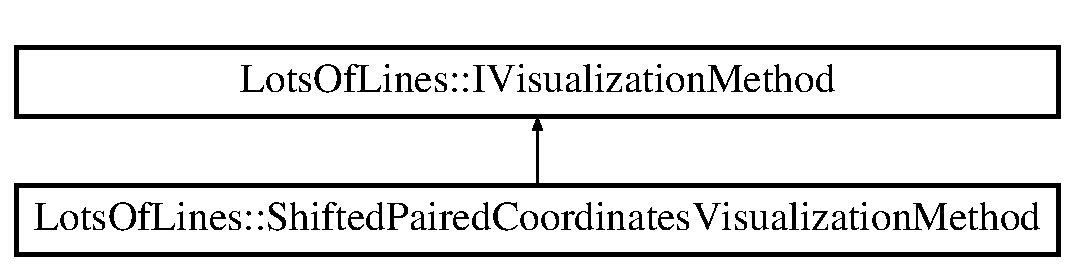
\includegraphics[height=2.000000cm]{class_lots_of_lines_1_1_shifted_paired_coordinates_visualization_method}
\end{center}
\end{figure}
\subsection*{Public Member Functions}
\begin{DoxyCompactItemize}
\item 
void \hyperlink{class_lots_of_lines_1_1_shifted_paired_coordinates_visualization_method_a5321d31a1b9d87b802080d263968bb30}{get\+Navigation\+Options} (\hyperlink{struct_lots_of_lines_1_1_navigation_options}{Navigation\+Options} \&options\+Out)\hypertarget{class_lots_of_lines_1_1_shifted_paired_coordinates_visualization_method_a5321d31a1b9d87b802080d263968bb30}{}\label{class_lots_of_lines_1_1_shifted_paired_coordinates_visualization_method_a5321d31a1b9d87b802080d263968bb30}

\begin{DoxyCompactList}\small\item\em Should return the navigation options for the rendering method (X scroll lock, etc) \end{DoxyCompactList}\item 
void \hyperlink{class_lots_of_lines_1_1_shifted_paired_coordinates_visualization_method_a8e77176927b8e3cd5e309636bb04f7a0}{get\+Default\+Options} (\hyperlink{class_lots_of_lines_1_1_visualization_options}{Visualization\+Options} \&options)\hypertarget{class_lots_of_lines_1_1_shifted_paired_coordinates_visualization_method_a8e77176927b8e3cd5e309636bb04f7a0}{}\label{class_lots_of_lines_1_1_shifted_paired_coordinates_visualization_method_a8e77176927b8e3cd5e309636bb04f7a0}

\begin{DoxyCompactList}\small\item\em Should fill an empty \hyperlink{class_lots_of_lines_1_1_visualization_options}{Visualization\+Options} object with the default options to use for the visualization method. This method will be called once when the visualization method is loaded in order to generate fields for the UI system. \end{DoxyCompactList}\item 
bool \hyperlink{class_lots_of_lines_1_1_shifted_paired_coordinates_visualization_method_a152e4c2e81fbb7dc6c3f41c24008faab}{generate\+V\+BO} (const std\+::shared\+\_\+ptr$<$ const \hyperlink{class_lots_of_lines_1_1_data_set}{Data\+Set} $>$ data\+Set, std\+::vector$<$ \hyperlink{struct_lots_of_lines_1_1_vertex}{Vertex} $>$ \&vertices\+Out, std\+::vector$<$ unsigned int $>$ \&indices\+Out, \hyperlink{class_lots_of_lines_1_1_rendering_system}{Rendering\+System} $\ast$driver, const \hyperlink{class_lots_of_lines_1_1_visualization_options}{Visualization\+Options} \&options)\hypertarget{class_lots_of_lines_1_1_shifted_paired_coordinates_visualization_method_a152e4c2e81fbb7dc6c3f41c24008faab}{}\label{class_lots_of_lines_1_1_shifted_paired_coordinates_visualization_method_a152e4c2e81fbb7dc6c3f41c24008faab}

\begin{DoxyCompactList}\small\item\em Generate a vertex buffer for the visualization. \end{DoxyCompactList}\end{DoxyCompactItemize}
\subsection*{Public Attributes}
\begin{DoxyCompactItemize}
\item 
const char $\ast$ {\bfseries S\+T\+EP} = \char`\"{}Distance of step\char`\"{}\hypertarget{class_lots_of_lines_1_1_shifted_paired_coordinates_visualization_method_ab86f2a4935bca666b6ec8b6f470e78b5}{}\label{class_lots_of_lines_1_1_shifted_paired_coordinates_visualization_method_ab86f2a4935bca666b6ec8b6f470e78b5}

\item 
const char $\ast$ {\bfseries A\+U\+T\+O\+\_\+\+S\+T\+EP} = \char`\"{}Auto step distance calculation\char`\"{}\hypertarget{class_lots_of_lines_1_1_shifted_paired_coordinates_visualization_method_ac7cd5880cd0caa625d40b173e761cbdc}{}\label{class_lots_of_lines_1_1_shifted_paired_coordinates_visualization_method_ac7cd5880cd0caa625d40b173e761cbdc}

\item 
const char $\ast$ {\bfseries H\+O\+R\+I\+Z\+O\+N\+T\+AL} = \char`\"{}Shift around horizontal line\char`\"{}\hypertarget{class_lots_of_lines_1_1_shifted_paired_coordinates_visualization_method_a6cad17ef30257ed3e1500bfb57d2387b}{}\label{class_lots_of_lines_1_1_shifted_paired_coordinates_visualization_method_a6cad17ef30257ed3e1500bfb57d2387b}

\item 
const char $\ast$ {\bfseries C\+O\+L\+L\+A\+P\+S\+ED} = \char`\"{}Collapse line to point\char`\"{}\hypertarget{class_lots_of_lines_1_1_shifted_paired_coordinates_visualization_method_ab82d61945baf2ab958e84bfef8db8ccf}{}\label{class_lots_of_lines_1_1_shifted_paired_coordinates_visualization_method_ab82d61945baf2ab958e84bfef8db8ccf}

\end{DoxyCompactItemize}


The documentation for this class was generated from the following files\+:\begin{DoxyCompactItemize}
\item 
D\+:/\+School/\+C\+W\+U/\+C\+S 481/\+Lots-\/of-\/\+Lines/source/\+Rendering\+System/Shifted\+Paired\+Coordinates\+Visualization\+Method.\+hpp\item 
D\+:/\+School/\+C\+W\+U/\+C\+S 481/\+Lots-\/of-\/\+Lines/source/\+Rendering\+System/Shifted\+Paired\+Coordinates\+Visualization\+Method.\+cpp\end{DoxyCompactItemize}

\hypertarget{class_ui___load_data_dialog}{}\section{Ui\+\_\+\+Load\+Data\+Dialog Class Reference}
\label{class_ui___load_data_dialog}\index{Ui\+\_\+\+Load\+Data\+Dialog@{Ui\+\_\+\+Load\+Data\+Dialog}}
Inheritance diagram for Ui\+\_\+\+Load\+Data\+Dialog\+:\begin{figure}[H]
\begin{center}
\leavevmode
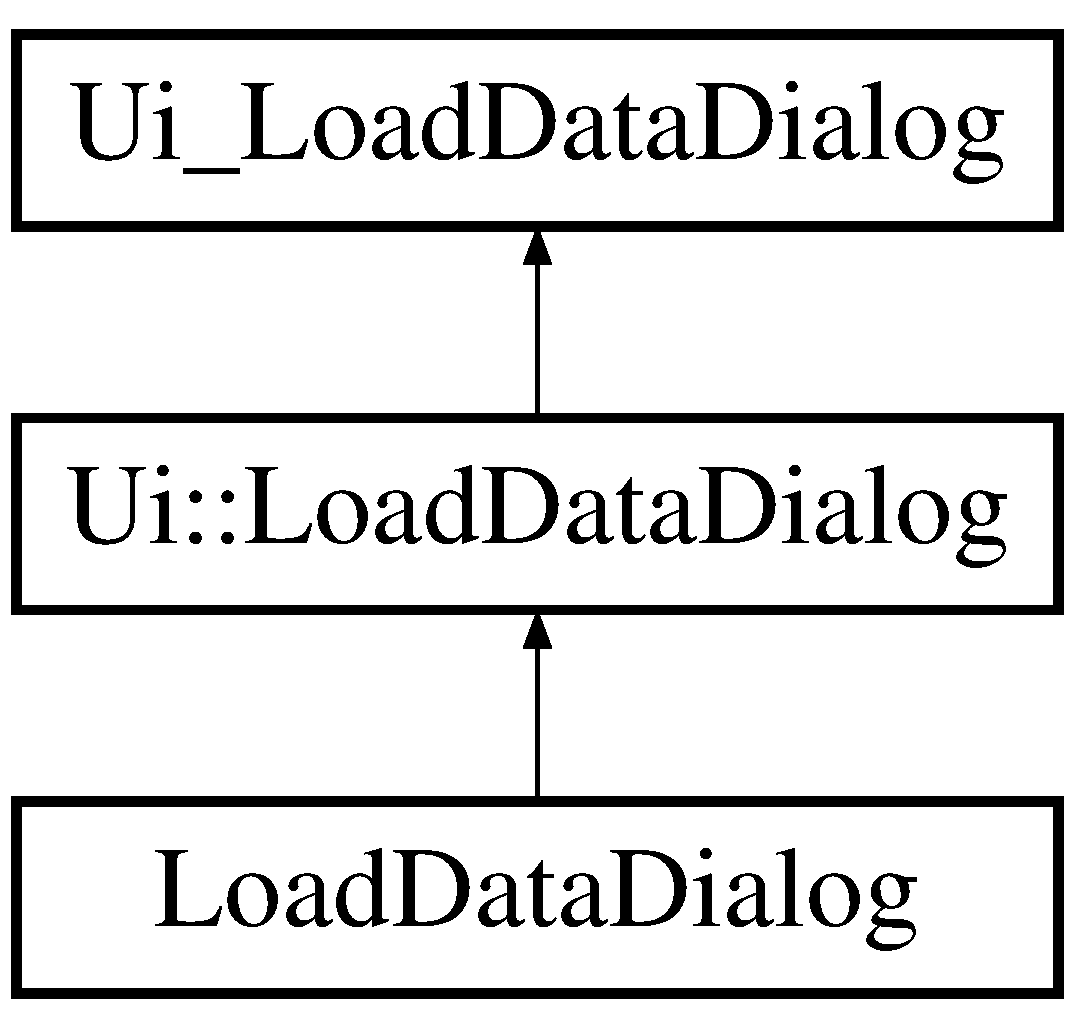
\includegraphics[height=3.000000cm]{class_ui___load_data_dialog}
\end{center}
\end{figure}
\subsection*{Public Member Functions}
\begin{DoxyCompactItemize}
\item 
void {\bfseries setup\+Ui} (Q\+Dialog $\ast$\hyperlink{class_load_data_dialog}{Load\+Data\+Dialog})\hypertarget{class_ui___load_data_dialog_ac7a58ea9a15abe76d52cfeaa890c0ecb}{}\label{class_ui___load_data_dialog_ac7a58ea9a15abe76d52cfeaa890c0ecb}

\item 
void {\bfseries retranslate\+Ui} (Q\+Dialog $\ast$\hyperlink{class_load_data_dialog}{Load\+Data\+Dialog})\hypertarget{class_ui___load_data_dialog_afead0ccca4f841f6977a86069187a805}{}\label{class_ui___load_data_dialog_afead0ccca4f841f6977a86069187a805}

\end{DoxyCompactItemize}
\subsection*{Public Attributes}
\begin{DoxyCompactItemize}
\item 
Q\+V\+Box\+Layout $\ast$ {\bfseries vertical\+Layout}\hypertarget{class_ui___load_data_dialog_a002c7621aef014c371701705db4b35d3}{}\label{class_ui___load_data_dialog_a002c7621aef014c371701705db4b35d3}

\item 
Q\+Line\+Edit $\ast$ {\bfseries selected\+File}\hypertarget{class_ui___load_data_dialog_ab1bc2c1ad7aa6615828c1812ad9bd190}{}\label{class_ui___load_data_dialog_ab1bc2c1ad7aa6615828c1812ad9bd190}

\item 
Q\+Group\+Box $\ast$ {\bfseries options\+Group\+Box}\hypertarget{class_ui___load_data_dialog_ad60f3985511153779fb0200ed7db5807}{}\label{class_ui___load_data_dialog_ad60f3985511153779fb0200ed7db5807}

\item 
Q\+Form\+Layout $\ast$ {\bfseries form\+Layout}\hypertarget{class_ui___load_data_dialog_a46eae3971f22aefe59e1695e305798a9}{}\label{class_ui___load_data_dialog_a46eae3971f22aefe59e1695e305798a9}

\item 
Q\+Label $\ast$ {\bfseries label\+\_\+2}\hypertarget{class_ui___load_data_dialog_aa0c326df664e0b73dab39092f5b46764}{}\label{class_ui___load_data_dialog_aa0c326df664e0b73dab39092f5b46764}

\item 
Q\+Combo\+Box $\ast$ {\bfseries normalization\+Method\+Select}\hypertarget{class_ui___load_data_dialog_a3b41717667b756a6a0ae78754f98a173}{}\label{class_ui___load_data_dialog_a3b41717667b756a6a0ae78754f98a173}

\item 
Q\+Check\+Box $\ast$ {\bfseries custom\+Class\+Column\+Checkbox}\hypertarget{class_ui___load_data_dialog_aebbf19e0034880f19ba7cb595d081b6a}{}\label{class_ui___load_data_dialog_aebbf19e0034880f19ba7cb595d081b6a}

\item 
Q\+Spin\+Box $\ast$ {\bfseries class\+Column\+Select}\hypertarget{class_ui___load_data_dialog_a4da2ea8a9a2fe384d95768bc8b33c6f6}{}\label{class_ui___load_data_dialog_a4da2ea8a9a2fe384d95768bc8b33c6f6}

\item 
Q\+Label $\ast$ {\bfseries label}\hypertarget{class_ui___load_data_dialog_aacc2412992d9d26b187bb2369df38516}{}\label{class_ui___load_data_dialog_aacc2412992d9d26b187bb2369df38516}

\item 
Q\+Line\+Edit $\ast$ {\bfseries ignored\+Columns\+Line\+Edit}\hypertarget{class_ui___load_data_dialog_ac0064cef81f27e637f029f7f507084b8}{}\label{class_ui___load_data_dialog_ac0064cef81f27e637f029f7f507084b8}

\item 
Q\+H\+Box\+Layout $\ast$ {\bfseries horizontal\+Layout\+\_\+2}\hypertarget{class_ui___load_data_dialog_af3b56d796d8ad28744d3e3c5985b0933}{}\label{class_ui___load_data_dialog_af3b56d796d8ad28744d3e3c5985b0933}

\item 
Q\+Spacer\+Item $\ast$ {\bfseries horizontal\+Spacer}\hypertarget{class_ui___load_data_dialog_ab7edf05ca3bd87d042689df3b0f0fe76}{}\label{class_ui___load_data_dialog_ab7edf05ca3bd87d042689df3b0f0fe76}

\item 
Q\+Push\+Button $\ast$ {\bfseries cancel\+Button}\hypertarget{class_ui___load_data_dialog_a002a831e7bd7f32444298a710f4e5bf7}{}\label{class_ui___load_data_dialog_a002a831e7bd7f32444298a710f4e5bf7}

\item 
Q\+Push\+Button $\ast$ {\bfseries ok\+Button}\hypertarget{class_ui___load_data_dialog_ad21125482fba8258459d8776b426caf4}{}\label{class_ui___load_data_dialog_ad21125482fba8258459d8776b426caf4}

\end{DoxyCompactItemize}


The documentation for this class was generated from the following file\+:\begin{DoxyCompactItemize}
\item 
D\+:/\+School/\+C\+W\+U/\+C\+S 481/\+Lots-\/of-\/\+Lines/source/\+Generated\+Files/ui\+\_\+\+Load\+Data\+Dialog.\+h\end{DoxyCompactItemize}

\hypertarget{class_ui___lots_of_lines_app_class}{}\section{Ui\+\_\+\+Lots\+Of\+Lines\+App\+Class Class Reference}
\label{class_ui___lots_of_lines_app_class}\index{Ui\+\_\+\+Lots\+Of\+Lines\+App\+Class@{Ui\+\_\+\+Lots\+Of\+Lines\+App\+Class}}
Inheritance diagram for Ui\+\_\+\+Lots\+Of\+Lines\+App\+Class\+:\begin{figure}[H]
\begin{center}
\leavevmode
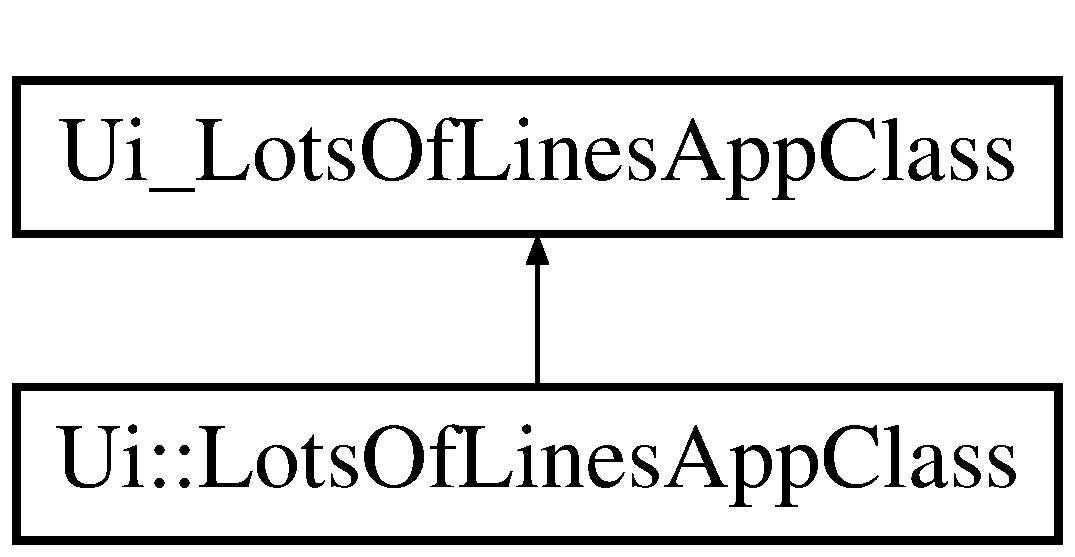
\includegraphics[height=2.000000cm]{class_ui___lots_of_lines_app_class}
\end{center}
\end{figure}
\subsection*{Public Member Functions}
\begin{DoxyCompactItemize}
\item 
void {\bfseries setup\+Ui} (Q\+Main\+Window $\ast$Lots\+Of\+Lines\+App\+Class)\hypertarget{class_ui___lots_of_lines_app_class_a0024f8e27a4af589e7748c4a47393657}{}\label{class_ui___lots_of_lines_app_class_a0024f8e27a4af589e7748c4a47393657}

\item 
void {\bfseries retranslate\+Ui} (Q\+Main\+Window $\ast$Lots\+Of\+Lines\+App\+Class)\hypertarget{class_ui___lots_of_lines_app_class_a0f5fa35889eb8640ff4467dba5ba3b07}{}\label{class_ui___lots_of_lines_app_class_a0f5fa35889eb8640ff4467dba5ba3b07}

\end{DoxyCompactItemize}
\subsection*{Public Attributes}
\begin{DoxyCompactItemize}
\item 
Q\+Action $\ast$ {\bfseries action\+Load}\hypertarget{class_ui___lots_of_lines_app_class_ac97798c51294047c272e1324ef33f9cc}{}\label{class_ui___lots_of_lines_app_class_ac97798c51294047c272e1324ef33f9cc}

\item 
Q\+Action $\ast$ {\bfseries action\+Windows}\hypertarget{class_ui___lots_of_lines_app_class_a798683f007bef85c52e27119e944a929}{}\label{class_ui___lots_of_lines_app_class_a798683f007bef85c52e27119e944a929}

\item 
Q\+Action $\ast$ {\bfseries action\+Visualization\+\_\+\+Options}\hypertarget{class_ui___lots_of_lines_app_class_aad8bfc8c7aede4c0aa8ed6047b989049}{}\label{class_ui___lots_of_lines_app_class_aad8bfc8c7aede4c0aa8ed6047b989049}

\item 
Q\+Action $\ast$ {\bfseries action\+Preferences}\hypertarget{class_ui___lots_of_lines_app_class_a75ef9939a78c24fbfca21829e7f155ea}{}\label{class_ui___lots_of_lines_app_class_a75ef9939a78c24fbfca21829e7f155ea}

\item 
Q\+Widget $\ast$ {\bfseries central\+Widget}\hypertarget{class_ui___lots_of_lines_app_class_a98725710eb52017e347d69ec91c9694e}{}\label{class_ui___lots_of_lines_app_class_a98725710eb52017e347d69ec91c9694e}

\item 
Q\+Grid\+Layout $\ast$ {\bfseries central\+Layout}\hypertarget{class_ui___lots_of_lines_app_class_ae881122b0181b6a1b68b0849c414c1cc}{}\label{class_ui___lots_of_lines_app_class_ae881122b0181b6a1b68b0849c414c1cc}

\item 
Q\+Menu\+Bar $\ast$ {\bfseries menu\+Bar}\hypertarget{class_ui___lots_of_lines_app_class_a3cdb6de1827e1c193c45574312cd2bfa}{}\label{class_ui___lots_of_lines_app_class_a3cdb6de1827e1c193c45574312cd2bfa}

\item 
Q\+Menu $\ast$ {\bfseries menu\+File}\hypertarget{class_ui___lots_of_lines_app_class_a6d0d769a036628da791dcd6d9840fe42}{}\label{class_ui___lots_of_lines_app_class_a6d0d769a036628da791dcd6d9840fe42}

\item 
Q\+Menu $\ast$ {\bfseries menu\+View}\hypertarget{class_ui___lots_of_lines_app_class_a6084609b9679bcaccb110c8ddf53ccd6}{}\label{class_ui___lots_of_lines_app_class_a6084609b9679bcaccb110c8ddf53ccd6}

\item 
Q\+Status\+Bar $\ast$ {\bfseries status\+Bar}\hypertarget{class_ui___lots_of_lines_app_class_a8551410529572ced3831cb7fb51a7ba0}{}\label{class_ui___lots_of_lines_app_class_a8551410529572ced3831cb7fb51a7ba0}

\item 
Q\+Dock\+Widget $\ast$ {\bfseries sidebar\+Dock\+Widget}\hypertarget{class_ui___lots_of_lines_app_class_a03c9a761b0441b48ce2a67f2be51934b}{}\label{class_ui___lots_of_lines_app_class_a03c9a761b0441b48ce2a67f2be51934b}

\item 
Q\+Widget $\ast$ {\bfseries dock\+Widget\+Contents}\hypertarget{class_ui___lots_of_lines_app_class_a88df3c4f5e4317d12dabedd3ac925402}{}\label{class_ui___lots_of_lines_app_class_a88df3c4f5e4317d12dabedd3ac925402}

\item 
Q\+V\+Box\+Layout $\ast$ {\bfseries vertical\+Layout}\hypertarget{class_ui___lots_of_lines_app_class_a235e4aa68f3469e48fcc150f15e8000f}{}\label{class_ui___lots_of_lines_app_class_a235e4aa68f3469e48fcc150f15e8000f}

\item 
Q\+Scroll\+Area $\ast$ {\bfseries sidebar\+Scroll\+Area}\hypertarget{class_ui___lots_of_lines_app_class_a2aaa5eb2c64ab54689f20c1d252a12ff}{}\label{class_ui___lots_of_lines_app_class_a2aaa5eb2c64ab54689f20c1d252a12ff}

\item 
Q\+Widget $\ast$ {\bfseries scroll\+Area\+Widget\+Contents}\hypertarget{class_ui___lots_of_lines_app_class_ac6cf5d1e55047e90e0c74939a7b79b9b}{}\label{class_ui___lots_of_lines_app_class_ac6cf5d1e55047e90e0c74939a7b79b9b}

\item 
Q\+V\+Box\+Layout $\ast$ {\bfseries vertical\+Layout\+\_\+2}\hypertarget{class_ui___lots_of_lines_app_class_acb92e8c4e7f71ff43864aba50b673d90}{}\label{class_ui___lots_of_lines_app_class_acb92e8c4e7f71ff43864aba50b673d90}

\item 
Q\+Group\+Box $\ast$ {\bfseries visualization\+Type\+Area}\hypertarget{class_ui___lots_of_lines_app_class_ad364201279203f97d385852457386a9b}{}\label{class_ui___lots_of_lines_app_class_ad364201279203f97d385852457386a9b}

\item 
Q\+V\+Box\+Layout $\ast$ {\bfseries visualization\+Type\+Layout}\hypertarget{class_ui___lots_of_lines_app_class_adb78f4619a2c3e0345f02612084dc17a}{}\label{class_ui___lots_of_lines_app_class_adb78f4619a2c3e0345f02612084dc17a}

\item 
Q\+Scroll\+Area $\ast$ {\bfseries options\+Scroll\+Area}\hypertarget{class_ui___lots_of_lines_app_class_a4ef3b74ff7f703281ecc5f6992404e4b}{}\label{class_ui___lots_of_lines_app_class_a4ef3b74ff7f703281ecc5f6992404e4b}

\item 
Q\+Widget $\ast$ {\bfseries scroll\+Area\+Widget\+Contents\+\_\+2}\hypertarget{class_ui___lots_of_lines_app_class_ab73a284f6badcfec7b10533d614b444b}{}\label{class_ui___lots_of_lines_app_class_ab73a284f6badcfec7b10533d614b444b}

\item 
Q\+V\+Box\+Layout $\ast$ {\bfseries options\+Scroll\+Layout}\hypertarget{class_ui___lots_of_lines_app_class_a94ed92b80042db434ca5ebf2df4ba0d7}{}\label{class_ui___lots_of_lines_app_class_a94ed92b80042db434ca5ebf2df4ba0d7}

\item 
Q\+Push\+Button $\ast$ {\bfseries load\+File\+Button}\hypertarget{class_ui___lots_of_lines_app_class_a8eb084892eddbe98ea89badc0528fbad}{}\label{class_ui___lots_of_lines_app_class_a8eb084892eddbe98ea89badc0528fbad}

\item 
Q\+Dock\+Widget $\ast$ {\bfseries data\+Table\+Dock}\hypertarget{class_ui___lots_of_lines_app_class_a94d34d4f3951cb3887cc854900fdbca9}{}\label{class_ui___lots_of_lines_app_class_a94d34d4f3951cb3887cc854900fdbca9}

\item 
Q\+Widget $\ast$ {\bfseries dock\+Widget\+Contents\+\_\+2}\hypertarget{class_ui___lots_of_lines_app_class_ab7b5476d27f06b04e888088487416d10}{}\label{class_ui___lots_of_lines_app_class_ab7b5476d27f06b04e888088487416d10}

\item 
Q\+Grid\+Layout $\ast$ {\bfseries grid\+Layout}\hypertarget{class_ui___lots_of_lines_app_class_a5410f9f7e4f7d905c13d6f91bf5f4a89}{}\label{class_ui___lots_of_lines_app_class_a5410f9f7e4f7d905c13d6f91bf5f4a89}

\item 
Q\+Tab\+Widget $\ast$ {\bfseries data\+Class\+Tabs}\hypertarget{class_ui___lots_of_lines_app_class_ae1baf7fa4580d8846f4e3d4b57e9627b}{}\label{class_ui___lots_of_lines_app_class_ae1baf7fa4580d8846f4e3d4b57e9627b}

\end{DoxyCompactItemize}


The documentation for this class was generated from the following file\+:\begin{DoxyCompactItemize}
\item 
D\+:/\+School/\+C\+W\+U/\+C\+S 481/\+Lots-\/of-\/\+Lines/source/\+Generated\+Files/ui\+\_\+\+Lots\+Of\+Lines\+App.\+h\end{DoxyCompactItemize}

\hypertarget{class_ui___preferences_dialog}{}\section{Ui\+\_\+\+Preferences\+Dialog Class Reference}
\label{class_ui___preferences_dialog}\index{Ui\+\_\+\+Preferences\+Dialog@{Ui\+\_\+\+Preferences\+Dialog}}
Inheritance diagram for Ui\+\_\+\+Preferences\+Dialog\+:\begin{figure}[H]
\begin{center}
\leavevmode
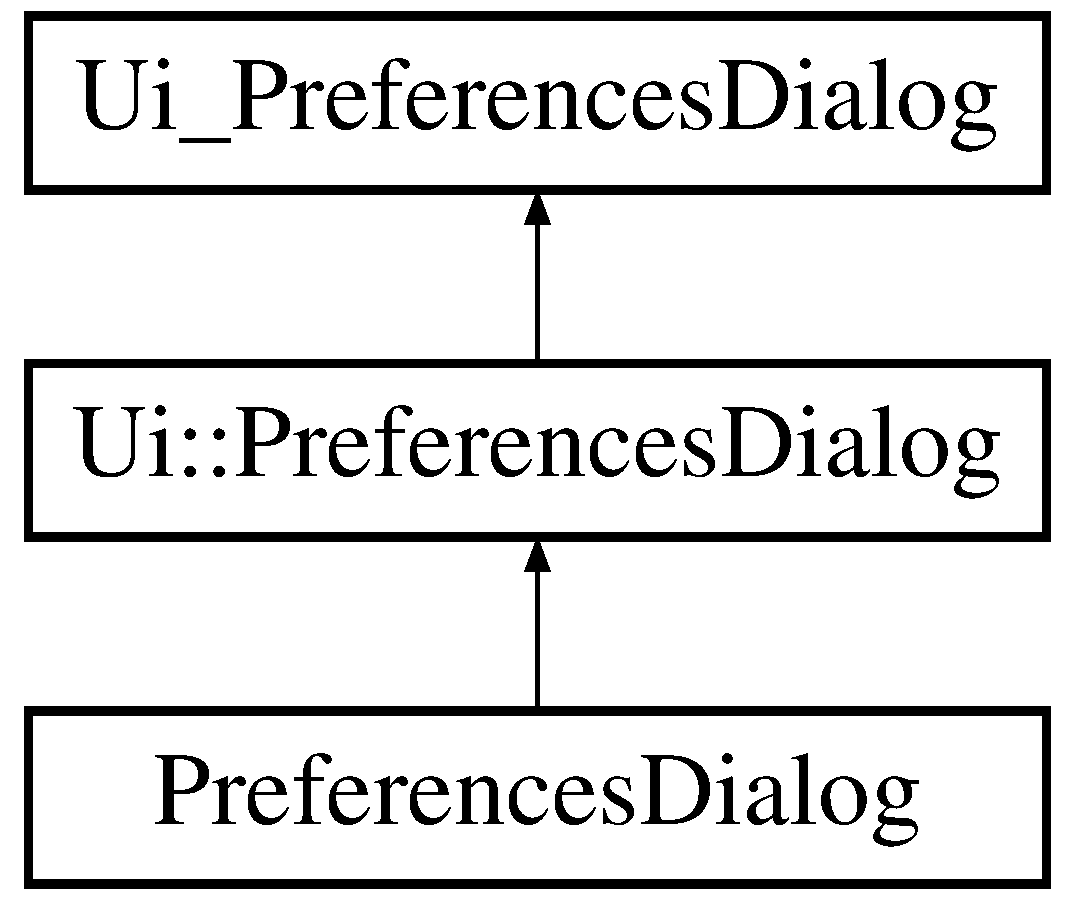
\includegraphics[height=3.000000cm]{class_ui___preferences_dialog}
\end{center}
\end{figure}
\subsection*{Public Member Functions}
\begin{DoxyCompactItemize}
\item 
void {\bfseries setup\+Ui} (Q\+Dialog $\ast$\hyperlink{class_preferences_dialog}{Preferences\+Dialog})\hypertarget{class_ui___preferences_dialog_ab2433bec54af4eb2a64c32241b994e6d}{}\label{class_ui___preferences_dialog_ab2433bec54af4eb2a64c32241b994e6d}

\item 
void {\bfseries retranslate\+Ui} (Q\+Dialog $\ast$\hyperlink{class_preferences_dialog}{Preferences\+Dialog})\hypertarget{class_ui___preferences_dialog_a05504e552435cca6485e5ee3a42ffe78}{}\label{class_ui___preferences_dialog_a05504e552435cca6485e5ee3a42ffe78}

\end{DoxyCompactItemize}
\subsection*{Public Attributes}
\begin{DoxyCompactItemize}
\item 
Q\+V\+Box\+Layout $\ast$ {\bfseries vertical\+Layout}\hypertarget{class_ui___preferences_dialog_ade30da332012acc7e9342c469ea9ced9}{}\label{class_ui___preferences_dialog_ade30da332012acc7e9342c469ea9ced9}

\item 
Q\+Tab\+Widget $\ast$ {\bfseries preferences\+Tabs}\hypertarget{class_ui___preferences_dialog_a17f3d8be9847cae3c0a5026be2cda41f}{}\label{class_ui___preferences_dialog_a17f3d8be9847cae3c0a5026be2cda41f}

\item 
Q\+Widget $\ast$ {\bfseries input\+Tab}\hypertarget{class_ui___preferences_dialog_a59a7e50717c7178825b430269b5c4657}{}\label{class_ui___preferences_dialog_a59a7e50717c7178825b430269b5c4657}

\item 
Q\+Widget $\ast$ {\bfseries rendering\+Tab}\hypertarget{class_ui___preferences_dialog_a103adee0971c954677c4d8dfb1652345}{}\label{class_ui___preferences_dialog_a103adee0971c954677c4d8dfb1652345}

\item 
Q\+H\+Box\+Layout $\ast$ {\bfseries hbox\+Layout}\hypertarget{class_ui___preferences_dialog_a593e29b0541f5b22ea623a82d47eae52}{}\label{class_ui___preferences_dialog_a593e29b0541f5b22ea623a82d47eae52}

\item 
Q\+Spacer\+Item $\ast$ {\bfseries spacer\+Item}\hypertarget{class_ui___preferences_dialog_a04494ffb0efea38588c361090e354c00}{}\label{class_ui___preferences_dialog_a04494ffb0efea38588c361090e354c00}

\item 
Q\+Push\+Button $\ast$ {\bfseries ok\+Button}\hypertarget{class_ui___preferences_dialog_a4cb797d31b7647bbe35eae1b5b9a4f1d}{}\label{class_ui___preferences_dialog_a4cb797d31b7647bbe35eae1b5b9a4f1d}

\item 
Q\+Push\+Button $\ast$ {\bfseries cancel\+Button}\hypertarget{class_ui___preferences_dialog_aa209554fae0085804c70b702a0f2aa8f}{}\label{class_ui___preferences_dialog_aa209554fae0085804c70b702a0f2aa8f}

\end{DoxyCompactItemize}


The documentation for this class was generated from the following file\+:\begin{DoxyCompactItemize}
\item 
D\+:/\+School/\+C\+W\+U/\+C\+S 481/\+Lots-\/of-\/\+Lines/source/\+Generated\+Files/ui\+\_\+\+Preferences\+Dialog.\+h\end{DoxyCompactItemize}

\hypertarget{struct_lots_of_lines_1_1_vertex}{}\section{Lots\+Of\+Lines\+:\+:Vertex Struct Reference}
\label{struct_lots_of_lines_1_1_vertex}\index{Lots\+Of\+Lines\+::\+Vertex@{Lots\+Of\+Lines\+::\+Vertex}}


\hyperlink{struct_lots_of_lines_1_1_vertex}{Vertex} structure for storing data to be sent to Open\+GL for rendering.  




{\ttfamily \#include $<$I\+Renderer.\+hpp$>$}

\subsection*{Public Member Functions}
\begin{DoxyCompactItemize}
\item 
{\bfseries Vertex} (float x, float y, unsigned int line\+Idx)\hypertarget{struct_lots_of_lines_1_1_vertex_a9c84b44d7dce68dfdc8fe910e162a008}{}\label{struct_lots_of_lines_1_1_vertex_a9c84b44d7dce68dfdc8fe910e162a008}

\end{DoxyCompactItemize}
\subsection*{Public Attributes}
\begin{DoxyCompactItemize}
\item 
float {\bfseries x}\hypertarget{struct_lots_of_lines_1_1_vertex_a3763bd4b8d3a32cebc6dfc99c5cebf4b}{}\label{struct_lots_of_lines_1_1_vertex_a3763bd4b8d3a32cebc6dfc99c5cebf4b}

\item 
float {\bfseries y}\hypertarget{struct_lots_of_lines_1_1_vertex_a48123278a323fed63e442f8854bf2947}{}\label{struct_lots_of_lines_1_1_vertex_a48123278a323fed63e442f8854bf2947}

\item 
float {\bfseries z}\hypertarget{struct_lots_of_lines_1_1_vertex_a152d16d21f3d761b4eb6683f9d93fe55}{}\label{struct_lots_of_lines_1_1_vertex_a152d16d21f3d761b4eb6683f9d93fe55}

\item 
std\+::uint32\+\_\+t \hyperlink{struct_lots_of_lines_1_1_vertex_af82ba390ca7177b67c293a18ea93e567}{data\+Class\+Index}\hypertarget{struct_lots_of_lines_1_1_vertex_af82ba390ca7177b67c293a18ea93e567}{}\label{struct_lots_of_lines_1_1_vertex_af82ba390ca7177b67c293a18ea93e567}

\begin{DoxyCompactList}\small\item\em Index of data class this vertice\textquotesingle{}s data belongs to. \end{DoxyCompactList}\item 
std\+::uint32\+\_\+t \hyperlink{struct_lots_of_lines_1_1_vertex_afc481025faf3d798a996a73c73c4da14}{flags}\hypertarget{struct_lots_of_lines_1_1_vertex_afc481025faf3d798a996a73c73c4da14}{}\label{struct_lots_of_lines_1_1_vertex_afc481025faf3d798a996a73c73c4da14}

\begin{DoxyCompactList}\small\item\em \hyperlink{struct_lots_of_lines_1_1_vertex}{Vertex} state flags. \end{DoxyCompactList}\item 
std\+::uint32\+\_\+t \hyperlink{struct_lots_of_lines_1_1_vertex_a219b266fe522f56ff9b861824b0cb9c6}{line\+Index}\hypertarget{struct_lots_of_lines_1_1_vertex_a219b266fe522f56ff9b861824b0cb9c6}{}\label{struct_lots_of_lines_1_1_vertex_a219b266fe522f56ff9b861824b0cb9c6}

\begin{DoxyCompactList}\small\item\em Index of line. \end{DoxyCompactList}\end{DoxyCompactItemize}


\subsection{Detailed Description}
\hyperlink{struct_lots_of_lines_1_1_vertex}{Vertex} structure for storing data to be sent to Open\+GL for rendering. 

The documentation for this struct was generated from the following file\+:\begin{DoxyCompactItemize}
\item 
D\+:/\+School/\+C\+W\+U/\+C\+S 481/\+Lots-\/of-\/\+Lines/source/\+Rendering\+System/I\+Renderer.\+hpp\end{DoxyCompactItemize}

\hypertarget{class_lots_of_lines_1_1_visualization_options}{}\section{Lots\+Of\+Lines\+:\+:Visualization\+Options Class Reference}
\label{class_lots_of_lines_1_1_visualization_options}\index{Lots\+Of\+Lines\+::\+Visualization\+Options@{Lots\+Of\+Lines\+::\+Visualization\+Options}}


Generic options class for visualizations.  




{\ttfamily \#include $<$Visualization\+Options.\+hpp$>$}

\subsection*{Public Member Functions}
\begin{DoxyCompactItemize}
\item 
bool \hyperlink{class_lots_of_lines_1_1_visualization_options_a8a3f354ffd70587b5756d3059d944fe6}{set\+Int} (const std\+::string \&name, int val)
\begin{DoxyCompactList}\small\item\em Set an integer option. \end{DoxyCompactList}\item 
bool \hyperlink{class_lots_of_lines_1_1_visualization_options_ae7021819f5b5d35aeeed3e267d716594}{set\+Double} (const std\+::string \&name, double val)
\begin{DoxyCompactList}\small\item\em Set a double option. \end{DoxyCompactList}\item 
bool \hyperlink{class_lots_of_lines_1_1_visualization_options_ac1c82295a5dfa5c6f4f143e7a9aa999c}{set\+String} (const std\+::string \&name, const std\+::string \&val)
\begin{DoxyCompactList}\small\item\em Set a string option. \end{DoxyCompactList}\item 
bool \hyperlink{class_lots_of_lines_1_1_visualization_options_aa5e71fe97363193855da10026ecc7432}{set\+Bool} (const std\+::string \&name, bool val)
\begin{DoxyCompactList}\small\item\em Set a boolean option. \end{DoxyCompactList}\item 
int \hyperlink{class_lots_of_lines_1_1_visualization_options_aac0c439a49fc160b49c57486c424a685}{get\+Int} (const std\+::string \&name, int default\+Val=0) const 
\item 
double \hyperlink{class_lots_of_lines_1_1_visualization_options_a679424b8e540c4745d27c3ec8e8bde45}{get\+Double} (const std\+::string \&name, double default\+Val=0) const 
\item 
std\+::string \hyperlink{class_lots_of_lines_1_1_visualization_options_a1fc1958635c86f4c8b4c8bdf84736200}{get\+String} (const std\+::string \&name, const std\+::string \&default\+Val=\char`\"{}\char`\"{}) const 
\item 
bool \hyperlink{class_lots_of_lines_1_1_visualization_options_a3b33ac20e7d79be9c15b74878996189e}{get\+Bool} (const std\+::string \&name, bool default\+Val=false) const 
\item 
void \hyperlink{class_lots_of_lines_1_1_visualization_options_a1e6f0ffb2bf3c49bdf8cfbf1ad5dd2d0}{clear} ()\hypertarget{class_lots_of_lines_1_1_visualization_options_a1e6f0ffb2bf3c49bdf8cfbf1ad5dd2d0}{}\label{class_lots_of_lines_1_1_visualization_options_a1e6f0ffb2bf3c49bdf8cfbf1ad5dd2d0}

\begin{DoxyCompactList}\small\item\em Remove all options. \end{DoxyCompactList}\item 
E\+\_\+\+O\+P\+T\+I\+O\+N\+\_\+\+T\+Y\+PE \hyperlink{class_lots_of_lines_1_1_visualization_options_ab0aa02018b8f80d8f9379cef84ec19f7}{get\+Option\+Type} (const std\+::string \&name)
\item 
const Option\+Type\+Map \& \hyperlink{class_lots_of_lines_1_1_visualization_options_a3c1438d905a5be4f0acb73f586298337}{list\+Options} ()
\end{DoxyCompactItemize}


\subsection{Detailed Description}
Generic options class for visualizations. 

\subsection{Member Function Documentation}
\index{Lots\+Of\+Lines\+::\+Visualization\+Options@{Lots\+Of\+Lines\+::\+Visualization\+Options}!get\+Bool@{get\+Bool}}
\index{get\+Bool@{get\+Bool}!Lots\+Of\+Lines\+::\+Visualization\+Options@{Lots\+Of\+Lines\+::\+Visualization\+Options}}
\subsubsection[{\texorpdfstring{get\+Bool(const std\+::string \&name, bool default\+Val=false) const }{getBool(const std::string &name, bool defaultVal=false) const }}]{\setlength{\rightskip}{0pt plus 5cm}bool Visualization\+Options\+::get\+Bool (
\begin{DoxyParamCaption}
\item[{const std\+::string \&}]{name, }
\item[{bool}]{default\+Val = {\ttfamily false}}
\end{DoxyParamCaption}
) const}\hypertarget{class_lots_of_lines_1_1_visualization_options_a3b33ac20e7d79be9c15b74878996189e}{}\label{class_lots_of_lines_1_1_visualization_options_a3b33ac20e7d79be9c15b74878996189e}
\begin{DoxyReturn}{Returns}
The value of the named bool option, or the specified default if it doesn\textquotesingle{}t exist. 
\end{DoxyReturn}
\index{Lots\+Of\+Lines\+::\+Visualization\+Options@{Lots\+Of\+Lines\+::\+Visualization\+Options}!get\+Double@{get\+Double}}
\index{get\+Double@{get\+Double}!Lots\+Of\+Lines\+::\+Visualization\+Options@{Lots\+Of\+Lines\+::\+Visualization\+Options}}
\subsubsection[{\texorpdfstring{get\+Double(const std\+::string \&name, double default\+Val=0) const }{getDouble(const std::string &name, double defaultVal=0) const }}]{\setlength{\rightskip}{0pt plus 5cm}double Visualization\+Options\+::get\+Double (
\begin{DoxyParamCaption}
\item[{const std\+::string \&}]{name, }
\item[{double}]{default\+Val = {\ttfamily 0}}
\end{DoxyParamCaption}
) const}\hypertarget{class_lots_of_lines_1_1_visualization_options_a679424b8e540c4745d27c3ec8e8bde45}{}\label{class_lots_of_lines_1_1_visualization_options_a679424b8e540c4745d27c3ec8e8bde45}
\begin{DoxyReturn}{Returns}
The value of the named double option, or the specified default if it doesn\textquotesingle{}t exist. 
\end{DoxyReturn}
\index{Lots\+Of\+Lines\+::\+Visualization\+Options@{Lots\+Of\+Lines\+::\+Visualization\+Options}!get\+Int@{get\+Int}}
\index{get\+Int@{get\+Int}!Lots\+Of\+Lines\+::\+Visualization\+Options@{Lots\+Of\+Lines\+::\+Visualization\+Options}}
\subsubsection[{\texorpdfstring{get\+Int(const std\+::string \&name, int default\+Val=0) const }{getInt(const std::string &name, int defaultVal=0) const }}]{\setlength{\rightskip}{0pt plus 5cm}int Visualization\+Options\+::get\+Int (
\begin{DoxyParamCaption}
\item[{const std\+::string \&}]{name, }
\item[{int}]{default\+Val = {\ttfamily 0}}
\end{DoxyParamCaption}
) const}\hypertarget{class_lots_of_lines_1_1_visualization_options_aac0c439a49fc160b49c57486c424a685}{}\label{class_lots_of_lines_1_1_visualization_options_aac0c439a49fc160b49c57486c424a685}
\begin{DoxyReturn}{Returns}
The value of the named integer option, or the specified default if it doesn\textquotesingle{}t exist. 
\end{DoxyReturn}
\index{Lots\+Of\+Lines\+::\+Visualization\+Options@{Lots\+Of\+Lines\+::\+Visualization\+Options}!get\+Option\+Type@{get\+Option\+Type}}
\index{get\+Option\+Type@{get\+Option\+Type}!Lots\+Of\+Lines\+::\+Visualization\+Options@{Lots\+Of\+Lines\+::\+Visualization\+Options}}
\subsubsection[{\texorpdfstring{get\+Option\+Type(const std\+::string \&name)}{getOptionType(const std::string &name)}}]{\setlength{\rightskip}{0pt plus 5cm}E\+\_\+\+O\+P\+T\+I\+O\+N\+\_\+\+T\+Y\+PE Visualization\+Options\+::get\+Option\+Type (
\begin{DoxyParamCaption}
\item[{const std\+::string \&}]{name}
\end{DoxyParamCaption}
)}\hypertarget{class_lots_of_lines_1_1_visualization_options_ab0aa02018b8f80d8f9379cef84ec19f7}{}\label{class_lots_of_lines_1_1_visualization_options_ab0aa02018b8f80d8f9379cef84ec19f7}
\begin{DoxyReturn}{Returns}
The type of the named option. 
\end{DoxyReturn}
\index{Lots\+Of\+Lines\+::\+Visualization\+Options@{Lots\+Of\+Lines\+::\+Visualization\+Options}!get\+String@{get\+String}}
\index{get\+String@{get\+String}!Lots\+Of\+Lines\+::\+Visualization\+Options@{Lots\+Of\+Lines\+::\+Visualization\+Options}}
\subsubsection[{\texorpdfstring{get\+String(const std\+::string \&name, const std\+::string \&default\+Val="""") const }{getString(const std::string &name, const std::string &defaultVal="") const }}]{\setlength{\rightskip}{0pt plus 5cm}std\+::string Visualization\+Options\+::get\+String (
\begin{DoxyParamCaption}
\item[{const std\+::string \&}]{name, }
\item[{const std\+::string \&}]{default\+Val = {\ttfamily \char`\"{}\char`\"{}}}
\end{DoxyParamCaption}
) const}\hypertarget{class_lots_of_lines_1_1_visualization_options_a1fc1958635c86f4c8b4c8bdf84736200}{}\label{class_lots_of_lines_1_1_visualization_options_a1fc1958635c86f4c8b4c8bdf84736200}
\begin{DoxyReturn}{Returns}
The value of the named string option, or the specified default if it doesn\textquotesingle{}t exist. 
\end{DoxyReturn}
\index{Lots\+Of\+Lines\+::\+Visualization\+Options@{Lots\+Of\+Lines\+::\+Visualization\+Options}!list\+Options@{list\+Options}}
\index{list\+Options@{list\+Options}!Lots\+Of\+Lines\+::\+Visualization\+Options@{Lots\+Of\+Lines\+::\+Visualization\+Options}}
\subsubsection[{\texorpdfstring{list\+Options()}{listOptions()}}]{\setlength{\rightskip}{0pt plus 5cm}const Option\+Type\+Map \& Visualization\+Options\+::list\+Options (
\begin{DoxyParamCaption}
{}
\end{DoxyParamCaption}
)}\hypertarget{class_lots_of_lines_1_1_visualization_options_a3c1438d905a5be4f0acb73f586298337}{}\label{class_lots_of_lines_1_1_visualization_options_a3c1438d905a5be4f0acb73f586298337}
\begin{DoxyReturn}{Returns}
Map of all option names and their types. 
\end{DoxyReturn}
\index{Lots\+Of\+Lines\+::\+Visualization\+Options@{Lots\+Of\+Lines\+::\+Visualization\+Options}!set\+Bool@{set\+Bool}}
\index{set\+Bool@{set\+Bool}!Lots\+Of\+Lines\+::\+Visualization\+Options@{Lots\+Of\+Lines\+::\+Visualization\+Options}}
\subsubsection[{\texorpdfstring{set\+Bool(const std\+::string \&name, bool val)}{setBool(const std::string &name, bool val)}}]{\setlength{\rightskip}{0pt plus 5cm}bool Visualization\+Options\+::set\+Bool (
\begin{DoxyParamCaption}
\item[{const std\+::string \&}]{name, }
\item[{bool}]{val}
\end{DoxyParamCaption}
)}\hypertarget{class_lots_of_lines_1_1_visualization_options_aa5e71fe97363193855da10026ecc7432}{}\label{class_lots_of_lines_1_1_visualization_options_aa5e71fe97363193855da10026ecc7432}


Set a boolean option. 

\begin{DoxyReturn}{Returns}
True on success, or returns false if the option has already been set as a different type. 
\end{DoxyReturn}
\index{Lots\+Of\+Lines\+::\+Visualization\+Options@{Lots\+Of\+Lines\+::\+Visualization\+Options}!set\+Double@{set\+Double}}
\index{set\+Double@{set\+Double}!Lots\+Of\+Lines\+::\+Visualization\+Options@{Lots\+Of\+Lines\+::\+Visualization\+Options}}
\subsubsection[{\texorpdfstring{set\+Double(const std\+::string \&name, double val)}{setDouble(const std::string &name, double val)}}]{\setlength{\rightskip}{0pt plus 5cm}bool Visualization\+Options\+::set\+Double (
\begin{DoxyParamCaption}
\item[{const std\+::string \&}]{name, }
\item[{double}]{val}
\end{DoxyParamCaption}
)}\hypertarget{class_lots_of_lines_1_1_visualization_options_ae7021819f5b5d35aeeed3e267d716594}{}\label{class_lots_of_lines_1_1_visualization_options_ae7021819f5b5d35aeeed3e267d716594}


Set a double option. 

\begin{DoxyReturn}{Returns}
True on success, or returns false if the option has already been set as a different type. 
\end{DoxyReturn}
\index{Lots\+Of\+Lines\+::\+Visualization\+Options@{Lots\+Of\+Lines\+::\+Visualization\+Options}!set\+Int@{set\+Int}}
\index{set\+Int@{set\+Int}!Lots\+Of\+Lines\+::\+Visualization\+Options@{Lots\+Of\+Lines\+::\+Visualization\+Options}}
\subsubsection[{\texorpdfstring{set\+Int(const std\+::string \&name, int val)}{setInt(const std::string &name, int val)}}]{\setlength{\rightskip}{0pt plus 5cm}bool Visualization\+Options\+::set\+Int (
\begin{DoxyParamCaption}
\item[{const std\+::string \&}]{name, }
\item[{int}]{val}
\end{DoxyParamCaption}
)}\hypertarget{class_lots_of_lines_1_1_visualization_options_a8a3f354ffd70587b5756d3059d944fe6}{}\label{class_lots_of_lines_1_1_visualization_options_a8a3f354ffd70587b5756d3059d944fe6}


Set an integer option. 

\begin{DoxyReturn}{Returns}
True on success, or returns false if the option has already been set as a different type. 
\end{DoxyReturn}
\index{Lots\+Of\+Lines\+::\+Visualization\+Options@{Lots\+Of\+Lines\+::\+Visualization\+Options}!set\+String@{set\+String}}
\index{set\+String@{set\+String}!Lots\+Of\+Lines\+::\+Visualization\+Options@{Lots\+Of\+Lines\+::\+Visualization\+Options}}
\subsubsection[{\texorpdfstring{set\+String(const std\+::string \&name, const std\+::string \&val)}{setString(const std::string &name, const std::string &val)}}]{\setlength{\rightskip}{0pt plus 5cm}bool Visualization\+Options\+::set\+String (
\begin{DoxyParamCaption}
\item[{const std\+::string \&}]{name, }
\item[{const std\+::string \&}]{val}
\end{DoxyParamCaption}
)}\hypertarget{class_lots_of_lines_1_1_visualization_options_ac1c82295a5dfa5c6f4f143e7a9aa999c}{}\label{class_lots_of_lines_1_1_visualization_options_ac1c82295a5dfa5c6f4f143e7a9aa999c}


Set a string option. 

\begin{DoxyReturn}{Returns}
True on success, or returns false if the option has already been set as a different type. 
\end{DoxyReturn}


The documentation for this class was generated from the following files\+:\begin{DoxyCompactItemize}
\item 
D\+:/\+School/\+C\+W\+U/\+C\+S 481/\+Lots-\/of-\/\+Lines/source/\+Rendering\+System/Visualization\+Options.\+hpp\item 
D\+:/\+School/\+C\+W\+U/\+C\+S 481/\+Lots-\/of-\/\+Lines/source/\+Rendering\+System/Visualization\+Options.\+cpp\end{DoxyCompactItemize}

\hypertarget{class_visualization_renderer_widget}{}\section{Visualization\+Renderer\+Widget Class Reference}
\label{class_visualization_renderer_widget}\index{Visualization\+Renderer\+Widget@{Visualization\+Renderer\+Widget}}
Inheritance diagram for Visualization\+Renderer\+Widget\+:\begin{figure}[H]
\begin{center}
\leavevmode
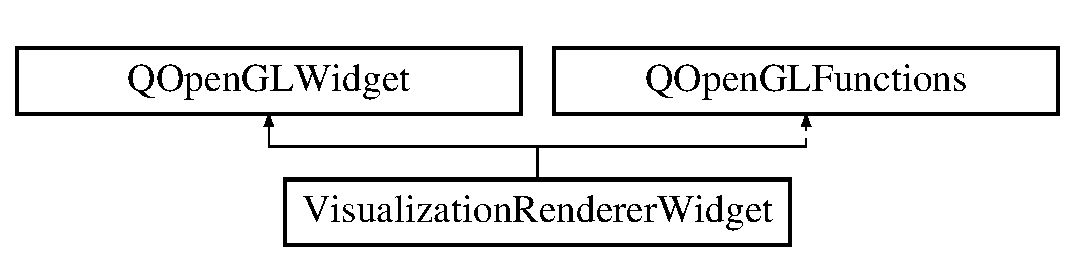
\includegraphics[height=2.000000cm]{class_visualization_renderer_widget}
\end{center}
\end{figure}
\subsection*{Public Member Functions}
\begin{DoxyCompactItemize}
\item 
{\bfseries Visualization\+Renderer\+Widget} (Q\+Widget $\ast$parent, std\+::function$<$ void(\hyperlink{class_lots_of_lines_1_1_rendering_system}{Lots\+Of\+Lines\+::\+Rendering\+System} $\ast$)$>$ init\+Callback=nullptr)\hypertarget{class_visualization_renderer_widget_a36920af3f1a80d491d14b48403f8656c}{}\label{class_visualization_renderer_widget_a36920af3f1a80d491d14b48403f8656c}

\item 
\hyperlink{class_lots_of_lines_1_1_rendering_system}{Lots\+Of\+Lines\+::\+Rendering\+System} $\ast$ {\bfseries get\+Rendering\+System} ()\hypertarget{class_visualization_renderer_widget_aa60e141abdbf2bbe2b157d784dabf73f}{}\label{class_visualization_renderer_widget_aa60e141abdbf2bbe2b157d784dabf73f}

\item 
void {\bfseries mouse\+Press\+Event} (Q\+Mouse\+Event $\ast$event\+Press)\hypertarget{class_visualization_renderer_widget_a4fec26286e0ce950e0fa001768d30772}{}\label{class_visualization_renderer_widget_a4fec26286e0ce950e0fa001768d30772}

\item 
void {\bfseries mouse\+Move\+Event} (Q\+Mouse\+Event $\ast$event\+Move)\hypertarget{class_visualization_renderer_widget_afd19b29b8e6ac4beeab2fcf460705073}{}\label{class_visualization_renderer_widget_afd19b29b8e6ac4beeab2fcf460705073}

\item 
void {\bfseries wheel\+Event} (Q\+Wheel\+Event $\ast$wheel\+Event)\hypertarget{class_visualization_renderer_widget_ae0b33c7ba9b3d56ad709dfbd43bc7a8a}{}\label{class_visualization_renderer_widget_ae0b33c7ba9b3d56ad709dfbd43bc7a8a}

\end{DoxyCompactItemize}
\subsection*{Protected Member Functions}
\begin{DoxyCompactItemize}
\item 
void {\bfseries initialize\+GL} ()\hypertarget{class_visualization_renderer_widget_a7c939c4bc260f17ca27f75cf8df19d2c}{}\label{class_visualization_renderer_widget_a7c939c4bc260f17ca27f75cf8df19d2c}

\item 
void {\bfseries resize\+GL} (int w, int h)\hypertarget{class_visualization_renderer_widget_a9302869ffc3ef25e22b364c3a53e5f9a}{}\label{class_visualization_renderer_widget_a9302869ffc3ef25e22b364c3a53e5f9a}

\item 
void {\bfseries paint\+GL} ()\hypertarget{class_visualization_renderer_widget_af87bb821a2d686d463da4b8761e327cd}{}\label{class_visualization_renderer_widget_af87bb821a2d686d463da4b8761e327cd}

\end{DoxyCompactItemize}
\subsection*{Protected Attributes}
\begin{DoxyCompactItemize}
\item 
\hyperlink{class_lots_of_lines_1_1_rendering_system}{Lots\+Of\+Lines\+::\+Rendering\+System} {\bfseries m\+\_\+rendering\+System}\hypertarget{class_visualization_renderer_widget_a16400c459c25a2d3d0065a7e21833aa8}{}\label{class_visualization_renderer_widget_a16400c459c25a2d3d0065a7e21833aa8}

\item 
std\+::function$<$ void(\hyperlink{class_lots_of_lines_1_1_rendering_system}{Lots\+Of\+Lines\+::\+Rendering\+System} $\ast$)$>$ {\bfseries m\+\_\+init\+Callback}\hypertarget{class_visualization_renderer_widget_a54b6bdf2a28b74d25fc1adbf49870d1a}{}\label{class_visualization_renderer_widget_a54b6bdf2a28b74d25fc1adbf49870d1a}

\end{DoxyCompactItemize}


The documentation for this class was generated from the following files\+:\begin{DoxyCompactItemize}
\item 
D\+:/\+School/\+C\+W\+U/\+C\+S 481/\+Lots-\/of-\/\+Lines/source/Visualization\+Renderer\+Widget.\+h\item 
D\+:/\+School/\+C\+W\+U/\+C\+S 481/\+Lots-\/of-\/\+Lines/source/Visualization\+Renderer\+Widget.\+cpp\end{DoxyCompactItemize}

\hypertarget{class_visualization_type_checkbox}{}\section{Visualization\+Type\+Checkbox Class Reference}
\label{class_visualization_type_checkbox}\index{Visualization\+Type\+Checkbox@{Visualization\+Type\+Checkbox}}
Inheritance diagram for Visualization\+Type\+Checkbox\+:\begin{figure}[H]
\begin{center}
\leavevmode
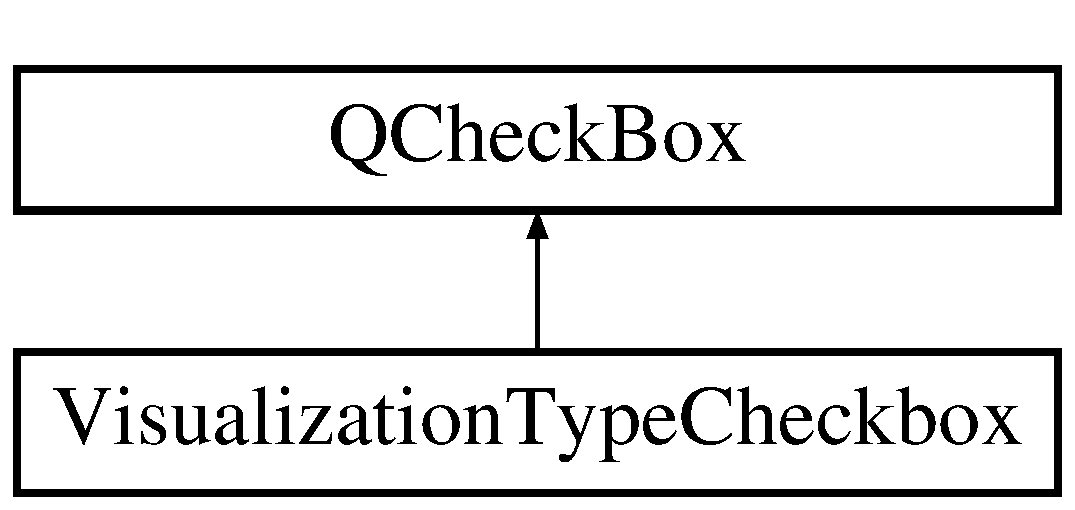
\includegraphics[height=2.000000cm]{class_visualization_type_checkbox}
\end{center}
\end{figure}
\subsection*{Public Member Functions}
\begin{DoxyCompactItemize}
\item 
{\bfseries Visualization\+Type\+Checkbox} (const Q\+String \&text, Q\+Widget $\ast$parent, Lots\+Of\+Lines\+::\+E\+\_\+\+V\+I\+S\+U\+A\+L\+I\+Z\+A\+T\+I\+O\+N\+\_\+\+T\+Y\+PE type)\hypertarget{class_visualization_type_checkbox_ae91c996fb27d74342b3e354c2f8f5bb6}{}\label{class_visualization_type_checkbox_ae91c996fb27d74342b3e354c2f8f5bb6}

\item 
Lots\+Of\+Lines\+::\+E\+\_\+\+V\+I\+S\+U\+A\+L\+I\+Z\+A\+T\+I\+O\+N\+\_\+\+T\+Y\+PE {\bfseries get\+Visualization\+Type} ()\hypertarget{class_visualization_type_checkbox_a68e39c617215ff97a3c113c44cca6031}{}\label{class_visualization_type_checkbox_a68e39c617215ff97a3c113c44cca6031}

\end{DoxyCompactItemize}


The documentation for this class was generated from the following file\+:\begin{DoxyCompactItemize}
\item 
D\+:/\+School/\+C\+W\+U/\+C\+S 481/\+Lots-\/of-\/\+Lines/source/Lots\+Of\+Lines\+App.\+cpp\end{DoxyCompactItemize}

%--- End generated contents ---

% Index
\backmatter
\newpage
\phantomsection
\clearemptydoublepage
\addcontentsline{toc}{chapter}{Index}
\printindex

\end{document}
